\documentclass[11pt, a4paper]{article}
\usepackage[nochapters]{classicthesis}
\usepackage[margin=42mm]{geometry}
\usepackage[utf8]{inputenc}
\usepackage[T1]{fontenc}
\usepackage{lmodern}
\usepackage[english]{babel}
\usepackage{graphicx}
\usepackage{url}
\usepackage{booktabs}
\usepackage{csquotes}
\usepackage{multirow}
\usepackage{amsfonts}
\usepackage{amsmath}
\usepackage{nicefrac}
\usepackage{microtype}
\usepackage{longtable}
\usepackage{array}
\usepackage{siunitx}
\usepackage{float}
\usepackage{caption}
\usepackage{subcaption}
\usepackage{tikz}
\usepackage{setspace}
\usepackage{enumitem}
\usepackage{xcolor}
\usepackage{natbib}
\usepackage{hyperref}
\usepackage{bookmark}

\definecolor{darkblue}{rgb}{0, 0, 0.5}

% ALL variable definitions (required by frontmatter.tex)
\def\thesistitle{Agent-Based Modeling of Autonomous Aerial Wildfire Suppression}
\def\subtitle{A Comparative Study of Drone Swarms, Traditional Aircraft, and Hybrid Systems}
\def\yourname{Kai Speidel}
\def\yourprogramme{Cognitive Science \& Artificial Intelligence}
\def\yourstudentnumber{2095270}
\def\finalmonth{June}
\def\finalyear{2025}
\def\supervisor{Dr. Travis J. Wiltshire}
\def\committee{Natalie Ranzhi Wei, MSc.}
\def\acknowledgments{Many thanks to my supervisor, Dr. Travis J. Wiltshire, for their invaluable guidance and support throughout this research project.  I would also like to express my gratitude to Natalie Ranzhi Wei, MSc., for their insightful feedback and expertise. Special appreciation goes to my family and friends for their encouragement and emotional support during this challenging but rewarding journey. Finally, I acknowledge the open-source community and the developers of Mesa, Python, and related libraries that made this research possible.}
\def\wordcount{8249}

\hypersetup{colorlinks=true,
            citecolor=darkblue,
            linkcolor=darkblue, 
            urlcolor=darkblue,
            pdfauthor=\yourname,
            pdftitle=\thesistitle}

\begin{document}
% DON'T TOUCH THIS FILE, THANKS!

\pagenumbering{gobble}
\thispagestyle{empty}

\newgeometry{margin=30mm}




\begin{center}
\hspace{0.75cm}
\includegraphics[scale=0.5]{logo.eps} \\
\vspace{5cm}
\huge\spacedallcaps{\thesistitle} \\ [0.5cm]
\Large\spacedallcaps{\subtitle} \\ [1.2cm]
\normalsize\spacedallcaps{\yourname{}} \\ [1cm]
\normalsize{\spacedlowsmallcaps{Thesis submitted in partial fulfillment}} \\
\normalsize{\spacedlowsmallcaps{of the requirements for the degree of}} \\
\normalsize{\spacedlowsmallcaps{Bachelor of Science in \yourprogramme{}}}\\
\vspace{0.5cm}
\normalsize{\spacedlowsmallcaps{Department of}}\\
\normalsize{\spacedlowsmallcaps{Cognitive Science \& Artificial Intelligence}}\\
\normalsize{\spacedlowsmallcaps{School of Humanities and Digital Sciences}} \\
\normalsize{\spacedlowsmallcaps{Tilburg University}} \\ [1.5cm]
\end{center}








\restoregeometry

\newpage

\begin{tabular}{l}
\noindent \spacedlowsmallcaps{student number} \\ [0.2cm]
\yourstudentnumber \\ [0.5cm]
\spacedlowsmallcaps{Committee} \\ [0.2cm]
\supervisor \\
\committee\\ [0.5cm]
\spacedlowsmallcaps{location} \\ [0.2cm]
Tilburg University    \\                        
School of Humanities and Digital Sciences \\
Department of Cognitive Science \& \\
Artificial Intelligence \\
Tilburg, The Netherlands \\ [0.5cm]
\spacedlowsmallcaps{date} \\ [0.2cm]
\today \\
\spacedlowsmallcaps{word count} \\ [0.2cm]
\wordcount



\end{tabular}
\vfill
\begin{tabular}{p{12cm}}
\spacedlowsmallcaps{acknowledgments} \\ [0.2cm]
\noindent \acknowledgments{}
\end{tabular}

\newpage \pagenumbering{arabic}

\title{\rmfamily\normalfont\spacedallcaps{\thesistitle}\\[0.2cm]
       \rmfamily\small\spacedallcaps{\subtitle}}
\author{\spacedlowsmallcaps{\yourname}}
\date{}

\maketitle

% Remove the duplicate title page stuff you had after frontmatter
% The frontmatter already creates title pages

\setcounter{page}{1}

\begin{abstract}
Wildfires pose a growing threat resulting from climate change, biodiversity loss, and human activity. This research explores economic and sustainable firefighting approaches using autonomous drone swarms, traditional aircraft, and hybrid models through agent-based modeling. A simulation framework created in Python using the Mesa library evaluates these methods, focusing on cost, sustainability (water, emissions), and computational efficiency. Drones, planes, fires, and resource stations were modeled as agents with parameters grounded in current research. Three path-finding algorithms (A*, Ant Colony Optimization, and Artificial Bee Colony) were implemented to guide drone behavior. The framework incorporates machine learning-based risk assessment to identify high-risk fire zones. This research contributes an open-source, modular simulation environment for evaluating aerial firefighting strategies, providing evidence-based insights for sustainable and efficient wildfire management practices.


\end{abstract}

\emph{``Each and every one of us can make changes in the way we live our lives and become part of the solution [to climate change]''} \\
--- Al Gore

\section{Data Source, Ethics, Code, and Technology (DSECT) Statement}
\label{sec:CodeOfCondunt}

This thesis uses only synthetically generated data through custom agent-based models created in Python using the Mesa library \citep{terMesa}. No external datasets, human/animal data, or consent were required. Simulation parameters are derived from cited research, and all figures and visualizations were created by the author using original simulation output. Code and documentation are available in the GitHub repository \citep{AgentBasedFirefightingModel_repository}.

The thesis follows the university's LaTeX template with Zotero \citep{zotero} for reference management. Generative AI tools (GitHub Copilot \citep{github_copilot}, Claude \citep{claudeai}, ChatGPT \citep{openai_chatgpt}) were used for feedback on author-created content, not for direct content generation. All conceptual, experimental, and implementation work was performed by the author.


\section{Introduction}
\label{sec:Introduction}

% - Why are wildfires problematic? 
% - How are they currently studied? 
% - What is ABM and why is it a powerful tool to study this phenomena? 
%- What are the components of your RQ that need to be explained? - Also see the results comment on RQs. 

Wildfires pose an escalating global threat, driven by climate change and human activity, with 96\% of wildfires being human-induced \citep{HybridAntColonyWildfire}. These events cause ecological, economic, and societal damage \citep{Saffre2022}, emitting over 2,000 megatons of carbon emissions globally in 2023 alone \citep{Lelis2024}. The UN Environment Program (UNEP) forecasts a 50\% increase by the end of the century in extreme wildfires if no countermeasures are taken \citep{Sullivan2022}. Escalating wildfire frequency also threatens agricultural productivity \citep{IPCC2023} and poses significant health risks through smoke exposure \citep{Finlay2012}. These combined effects make wildfires one of the most urgent environmental and societal challenges today.

Wildfire research traditionally employs different methodological approaches, with different advantages and limitations. Historical analysis creates the foundation of wildfire research. Researchers examine fire records, satellite imagery, and climate data to identify patterns and correlations between environmental factors and fire behavior \citep{copernicus-wildfires,IPCC2023}. These studies offer valuable insights into long-term fire cycles and climate relationships, but their retrospective nature limits their adaptability to the accelerating climate change. 

Controlled wildfire burns offer scientists valuable real-world data about fire physics and suppression in a controlled environment \citep{wildland}. These field studies are limited by safety concerns, high costs, and their impossibility of testing extreme scenarios or comparing multiple suppression strategies simultaneously.

For decades, traditional aerial firefighting and data collection relied heavily on manned aircraft such as fixed-wing planes \citep{janney2012airtankers}. These aircraft deliver water or fire retardant directly to the fire zones, often in dangerous conditions with limited visibility. Their effectiveness comes with safety constraints, high operational costs and substantial carbon emissions \citep{spicerRapidMeasurementEmissions2009}.

Recent technological advancements have sparked growing interest in autonomous drone systems for wildfire suppression. Modern drone technology potentially offers operation in extreme conditions without risking human life, while being lower in costs and emissions. Research done by \citet{Yan2024} effectively demonstrates the possibility of using coordinated swarm behavior to detect forest fires. Current research presents promising applications, such as new suppression techniques like the ``fireball'' by \citet{fireBalls}.

While the development is promising, especially with more applied drone applications being tested, scientists have also turned to simulation studies as they provide evidence for fire spread behavior at a lower cost. The fire area simulator ``FARSITE'' \citep{FARSITE}, established a baseline for future work, such as the model proposed by \citet{integrated_simulation}, which integrates fire simulation with optimization-based analysis. This is where Agent-Based Modeling (ABM) plays an important role.

Based on \citet{wilensky2015introduction}, ABM is defined as a methodology for conducting computer-based experiments that enables the study of complex systems by simulating the actions and interactions of autonomous agents within natural, social, or engineered contexts. These dynamic interactions generate complex, system-level patterns, commonly referred to as \textit{emergent behavior}. In wildfire research, ABM enables researchers to model fires, suppression vehicles, and environmental factors as independent agents with distinct behaviors and decision-making capabilities. This approach captures the emergent properties of complex firefighting scenarios that would be difficult or impossible to study through traditional analytical methods or real-world experiments. ABM provides evidence through the analysis of emergent behavior, which can inform real-world firefighting strategies. Additionally, it allows for the modeling of dynamic systems where multiple autonomous agents must coordinate to achieve common objectives under controlled conditions, making it particularly suited for the goal of this thesis. 

Path-finding algorithms are computational methods designed to find efficient routes between two points in a space, often while avoiding obstacles or minimizing costs (such as time, distance, or energy). These algorithms often use heuristics, which are informed problem-solving techniques, to efficiently explore potential solutions in a solution space under the premise that exploring every possible solution is computationally infeasible. When the heuristic is admissible, it guarantees that the algorithm will find an optimal path \citep{heuristic}. 

As wildfires grow in intensity and frequency, traditional suppression methods face increasing limitations. Agent-Based Modeling (ABM) presents a powerful tool for simulating complex scenarios involving autonomous firefighting drones. However, there is limited research directly comparing different suppression strategies, such as drone swarms, hybrid systems, and traditional aircraft, within the same simulation environment.

\subsection{Research Question}
Given the evident need for sustainable wildfire suppression and promising potential of autonomous approaches, this research addresses the following question:
\begin{quote}
\emph{How can agent-based modeling be used to evaluate and optimize autonomous aerial wildfire suppression strategies across drone, plane, and hybrid systems, using path-finding algorithms to assess effectiveness, efficiency, and sustainability?}
\end{quote}

\noindent Accordingly, the following sub-questions are addressed: 

\begin{itemize}
    \item[RQ1] \emph{How do path-finding algorithms influence the firefighting performance of drone swarms in ABMs?}
    \item[RQ2] \emph{How do drone swarms, hybrid systems, and planes compare in wildfire suppression?}
    \item[RQ3] \emph{What trade-offs emerge among suppression effectiveness, efficiency and sustainability?}
\end{itemize}

\subsection{Findings}

This thesis presents a robust open-source agent-based simulation framework developed in Python using the Mesa library. Its object-oriented and well-documented architecture promotes interdisciplinary research. The framework provides researchers and relevant stakeholders, such as policymakers, emergency response planners, and environmental scientists, with a flexible tool to build on top of and evaluate custom aerial vehicle models and coordination strategies across a range of simulated scenarios. Its public availability offers benefit, especially in resource-limited regions, by enabling access to advanced simulation and planning tools.

In the scope of this thesis, autonomous drone swarms, firefighting planes,  and a hybrid system are simulated. These approaches have been compared, focusing on effectiveness, cost, emissions, and water usage. The results indicate intricate patterns emerging from different approaches, showing that that hybrid systems might offer the best trade-off regarding effectiveness and sustainability.

\section{Related Work}

\subsection{The Importance of preventing Wildfires}
As previously mentioned, wildfires are increasing in frequency and intensity, creating devastating destruction. In addition to ecological damage, the economic impact is substantial. While the annual cost of wildfire management in the U.S. is estimated to range from \$7.6 billion to \$62.8 billion, the economic damage is estimated between \$63.5 billion to \$285.0 billion \citep{Afghah2019}. This highlights the need for practical, cost-effective and quick solutions. Pursuing sustainable approaches is essential, as traditional methods are costly and emit a lot of CO\textsubscript{2} \citep{Saffre2022}. The ecological consequences, especially on the agricultural sector, are recognized as a societal threat \citep{grassland_Wildfires,IPCC2023}. 

\subsection{Traditional Methods}

Aerial firefighting, introduced in the 1950s using repurposed military aircraft, evolved significantly in the 1960s with the introduction of specialized tactics and retardants \citep{janney2012airtankers,struminskaFlightPerformanceAnalysis2024}. These methods advancements enabled access to remote areas feasible and led to the development of aircraft specifically for firefighting roles \citep{struminskaFlightPerformanceAnalysis2024,LockheedSuperHercules}. Modern fleets include a range of aerial vehicles for specific operational tasks \citep{FleetInformationFirefighting}. 

Despite their effectiveness, these methods are costly, risky for the crew involved, and operationally demanding \citep[p. 1896]{struminskaFlightPerformanceAnalysis2024}. Emissions from aircraft like the C-130 Hercules are immense and difficult to quantify \citep{LockheedC130Hercules2022,spicerRapidMeasurementEmissions2009}.
Coordination and situational awareness limitations, especially under smoke, wind, and turbulence, further complicate human-led missions \citep{struminskaFlightPerformanceAnalysis2024}. 
These challenges motivate the study of autonomous systems, which promise real-time data sharing, coordinated swarm behavior, and quick adaptation to changing fire conditions. Given the increasing frequency and intensity of wildfires \citep{copernicus-wildfires,IPCC2023,grassland_Wildfires}, the development of more responsive and autonomous strategies is of high importance.

\subsection{Emergence of Drone-Based Solutions}

With advancement of global technologies in recent years, drone systems went through significant development in terms of functionality and operational capabilities. Unmanned Aerial Vehicles (UAV) are increasingly integrated across a range of industrial sectors, including agriculture, healthcare, logistics, and military operations \citep{emimiCurrentOpportunitiesChallenges2023}. Their main advantages are adaptability, precision, and cost-efficiency, however these benefits are accompanied by persistent regulatory, operational, and ethical challenges \citep{emimiCurrentOpportunitiesChallenges2023}.

The research conducted by \citet*{Saffre2022} demonstrates that autonomous drone swarms are capable of effectively containing wildfires while also reducing greenhouse gas emissions compared to traditional methods \citep{Saffre2022}. In addition, drones are increasingly recognized for their energy efficiency, making them a promising solution for sustainable disaster response strategies \citep{stolaroffEnergyUseLife2018}.

Emerging drone-specific firefighting techniques further expand the potential of UAVs in this domain. For example, the ``Firefighting Ball'' present a novel condemning technology designed specifically for aerial deployment via drones \citep{fireBalls}. Building upon this, an autonomous system that integrates the fireball concept into a coordinated drone-based suppression framework got introduced \citep{alkhatibProposedAutomaticForest2024}.

The effectiveness of drone-based firefighting systems is evident, specifically in terms of cost-efficiency and lower emissions. However, for these systems to achieve optimal performance, early wildfire detection is crucial. Fast and confident identification of fire outbreaks is one of the most critical factors in minimizing damage, especially during the initial stages of a wildfire event \citep{Sudhakar2020}.
In comparison, traditional risk assessment measures are delayed and have low confidence, especially in remote areas \citep{Afghah2019}, highlighting the potential for improvement in autonomous data collection \citep{Lelis2024} with drones.

The low cost and compact size of drones also make simultaneous deployment of multiple units possible, therefore enabling coordinated swarm behavior, which is a logical progression in UAV-based wildfire management \citep{MetaanalysisHumansystemInterfaces}. 

Swarm behavior supports the application of bio-inspired algorithms, such as Ant Colony Optimization \citep{HybridAntColonyWildfire} and Artificial Bee Colony algorithms \citep{karaboga2007abc}, which increase in effectiveness as swarm size increases. These algorithms allow drones to efficiently compute optimal paths to fire sites, managing speed and resource use. \citet*{MetaanalysisHumansystemInterfaces} identified this growing research area to become increasingly important in addressing complex real-world challenges such as wildfire detection and suppression.
While the physical and algorithmic capabilities of drones develop rapidly, coordinating a swarm of autonomous UAVs in uncertain environments, especially extreme ones such as wildfire zones, remains a significant challenge. These systems involve many interacting agents reacting to various parameters. This introduces a level of behavioral and environmental complexity that is difficult to model using top-down or deterministic approaches. As a result ABM offers a framework to simulate and test swarm coordination strategies in complex domains like wildfire suppression.

\subsection{Agent-Based Modeling}
ABM is a computational methodology used for conducting experiments that enable the study of complex systems by simulating actions and interactions of autonomous agents within different domains  \citep{wilensky2015introduction}. Each agent follows a set of simple rules, and through repeated interaction with other agents and their environment, ``sustainable patterns can emerge in systems that are completely described by simple rules'' \citep[p.5]{intro_to_abm}. These dynamic interactions generate complex, system-level patterns, commonly referred to as emergent behavior. These emergent patterns reveal dynamics that are difficult to predict analytically, providing valuable insights for informed decision-making.
ABM is grounded in the principles of complexity theory, which studies how individual agents interact within a system, leading to emergent behaviors and patterns. As \citet*{wilensky2015introduction} explained, complexity theory provides a framework for understanding systems in which ``order emerges without central control'', making it specifically relevant for wildfire management, where conditions are dynamic and decisions must be made in real time without centralized control. By modeling planes and drones as autonomous agents, ABM provides a framework where each agent is equipped with its own sensors, movement capabilities, and objectives (e.g., resource management or fire suppression). The simulated environment can be defined and modeled to represent real-world elements such as terrain, vegetation, and fire spread mechanics, making it a powerful tool for investigating wildfire response strategies.

NetLogo's ``Forest Fire'' simulation demonstrates how simple ignition and spread rules can mimic the dynamic growth of wildfires \citep{wilensky2015introduction}. Recent implementations demonstrated ABM as a valuable tool to understand forest fires through simulating complex environments and testing different suppression strategies. For instance, \citet*{MorenoEspino2025} applies ABM through the GAMA platform \citep{Gamma} to simulate wildfire propagation by modeling fire cells, vegetation, and weather as interacting agents. Their approach integrates geographic data, reflecting real-world terrain, highlighting how environmental variables like wind speed influence fire spread and intensity. Similarly, \citet*{Dorrer_2020} presented an ABM that integrates a simulated environment onto actual terrain data, combining both fire agents and firefighting agents. Their model provides insights into fire control strategies by demonstrating how emergent behaviors from the agents' interaction with the spreading fire can give evidence for informed resource allocation and decision-making.

These studies demonstrate the relevance of ABM in capturing the dynamics of wildfire events. Building on this foundation, this thesis takes a comparative approach to evaluate coordination strategies by contrasting autonomous drone systems with plane only and hybrid models. However, the effectiveness of autonomous drone swarms in ABM simulations for wildfire suppression depends on the path-finding algorithms which dictate the agents movement and coordination strategies.

\subsection{Path-finding Algorithms}

In the context of this thesis, path-finding algorithms are designed to enable the agents to balance competing objectives: minimizing travel time to fire sites, avoid collisions with other agents, and reducing resource consumption, all while adapting to dynamic fire spread.

\paragraph{A* Search} The A* algorithm, introduced by \citet*{heuristic}, is the foundation of modern heuristic path-finding, It calculates:
\begin{equation}
  f(n) = g(n) + h(n)
\end{equation}

where $g(n)$ represents the actual cost from the start node to node $n$, and $h(n)$ is the heuristic estimate of the cost from node $n$ to the goal. When the heuristic $h(n)$ is admissible (never overestimates the true cost) and consistent, A* guarantees finding the shortest path while expanding fewer nodes than uninformed search methods \citep{heuristic}. 
While A* performs well in known environments, it faces limitations in dynamic scenarios where conditions change rapidly and multiple agents must coordinate simultaneously.

This is where nature-inspired algorithms offer an alternative. Nature-inspired path-finding algorithms draw their inspiration and theoretical concepts from biological systems that exhibit efficient collective navigation and optimization behaviors. These approaches are specifically valuable in wildfire suppression contexts because they enable decentralized decision-making, adaptive behavior, and emergent coordination, making them essential for effective swarm operations in unpredictable environments.

\paragraph{Ant Colony Optimization} (ACO) mimics the foraging behavior of ant colonies, where individual ants leave pheromone trails to guide other ants towards food sources \citep{ACO}. The original ACO algorithm, developed by \citet*{ACO}, has since been applied across various optimization domains \citep{ACO_recent_advances}.
In drone applications, virtual pheromones can represent fire intensity levels or successful suppression paths. This mechanism enables drones to converge on high-priority areas while maintaining swarm coordination.
\citet*{HybridAntColonyWildfire} demonstrates how ACO can be applied in wildfire scenarios by developing a system that coordinates multiple agents for fire prevention and mitigation. ACO's main advantage lies in its ability to find near-optimal solutions through emergent collective intelligence without requiring centralized control, making it perfectly suitable for wildfire suppression in ABM simulations.


\paragraph{Artificial Bee Colony} (ABC) is a swarm-based meta-heuristic algorithm. Inspired by the behavior of honeybee swarms, the algorithm simulates the decision-making processes of honeybee colonies during nectar foraging \citep{karaboga2007abc}. The algorithm divides the swarm into three types of bees: employed bees that exploit existing food sources, onlooker bees that select among these sources based on information shared by employed bees, and scout bees that search for new food sources randomly when existing ones are exhausted \citep{karaboga2007abc}.
In wildfire suppression contexts, this translates to drones that can exploit known fire locations (employed behavior), explore new fire areas based on information from other drones (onlooker behavior), and conduct random searches when no fires are detected (scout behavior). This behavioral division enables effective load balancing between exploitation of current fire sites and exploration of potential new outbreaks. This property highlights the strength of ABC, which lies in its inherent balance of exploration and exploitation, making it particularly useful for dynamic environments where fire conditions and resource availability change rapidly.

These nature-inspired algorithms provide the needed computational foundation for autonomous coordination. However, as demonstrated in the following sections the integration of human oversight with the mentioned autonomous capabilities can further enhance system performance and adaptability.

\subsection{Human-Drone Teaming}

As the complexity of drone systems is increasing, maintaining effective coordination presents a growing trade-off between autonomy, control, and performance. Human drone teaming (HDT) offers a promising middle ground by balancing centralized oversight with distributed decision-making \citep{asavasirikulkij2023human_Workload}. Integrating humans into the loop enhances strategy flexibility while reducing cognitive load. \citet{SAT_first} demonstrate that systems, where human operators oversee multiple UAVs and intervene only when necessary, enhance both situational awareness and mission reliability. This supervised control enables operators to make strategic decisions without managing each drone independently, thus reducing cognitive load and improving the flexibility of the operation. Similarly, \citet*{lewisHumanFactorsIssues2012} show that human operators can effectively direct swarm behavior by influencing a subset of agents rather than all agents at once.
These findings suggest that humans are essential for providing strategic decisions and maintaining oversight, while autonomous systems manage local coordination and provide situational data. This division of tasks supports flexible and informed decision-making in a highly complex environment.
In this thesis, such interactions are explored in a simulated ABM environment, where the agents provide data about the dynamic environment and respond to changing conditions. The emergent interactions and collected data can be used for informed decision-making by providing evidence about drone and plane behavior.

\subsection{Summary}

While ABM research is growing especially in the field of swarm behavior and novel techniques to apply UAVs in extreme situations, a research gap remains in comparative simulation studies that evaluate different aerial firefighting techniques within the same framework. Current literature often focuses on individual aspects instead of systematic comparative analysis.

Furthermore, while nature-inspired path-finding algorithms show promise for autonomous coordination, their practical application and comparative performance in wildfire suppression scenarios remain underexplored in ABM. This thesis addresses these gaps by developing a comprehensive simulation environment that enables direct comparison of autonomous drone systems, traditional aircraft, and hybrid approaches, while integrating path-finding algorithms to evaluate their combined impact on suppression effectiveness and sustainability. Sustainability is assessed using metrics water consumption, carbon emissions (kg CO\textsubscript{2}), and operational costs as metrics (see Methodology section).


\section{Methodology}
\label{sec:Methodology}

This study uses a simulation-based approach to evaluate different suppression strategies. At its core, the methodology involves agent-based modeling, path-finding algorithms, and machine learning-based risk analysis. The goal is to determine the operational, environmental, and economic effectiveness of drones, planes, and hybrid firefighting systems. All simulations are created using Mesa \citep{terMesa}, as it is ideal to study complex emergent behavior. Given the complexity inherent in agent-based simulation studies, a detailed description of the initialization process and agent setup is provided to ensure clarity, reproducibility, and transparency.

\subsection{Simulation Design and Setup}
\paragraph{Environment} The simulated environment consists of a 250×250 discrete grid (62,500 total cells) representing the landscape where wildfire events occur, where one cell is equivalent to 10 meters. This creates a simulation area of 2.5 km × 2.5 km (6.25 km\textsuperscript{2}), representing a realistic wildfire scenario. This grid size was selected to balance computational efficiency while maintaining an appropriate size for meaningful agent interactions and fire dynamics. Each cell tracks state information about occupancy status, fire state, and resource station allocation. The simulation proceeds in predefined steps (1000). Fires can ignite, grow in intensity, and spread to adjacent cells probabilistically. Fire suppression agents attempt to extinguish them while managing internal resource constraints. (e.g., water supply, energy). 
\paragraph{Agent Configuration} To answer RQ2's comparative research focus, the simulation employs three different suppression approaches, following ABM methodology introduced by \citet*{wilensky2015introduction}.
\begin{enumerate}
  \item \textbf{Drone-only approach}: 30 autonomous drone agents are employed. Reflecting a frequently used swarm size in swarm optimization studies (Z\textsubscript{max} = 30) \citep{swarm1_kozlov2022information,swarm2_optimization_drone}. This size ensures meaningful coordination strategies while balancing computational efficiency. The drones are initiated with an individual water capacity of \SI{50}{\liter} which results in a total swarm capacity of \SI{1500}{\liter}. RQ1 is addressed by comparing different path-finding algorithms and analyzing how their distinct behaviors influence emergent wildfire suppression outcomes.
  \item \textbf{Plane-Only}: 4 firefighting aircraft are employed, reflecting a realistic firefighting fleet in extreme scenarios \citep{sherryAerialFireFighting2025}. Given an individual water capacity of \SI{18184}{\liter} per plane, the total fleet capacity is \SI{72736}{\liter}. Considering that firefighting planes are the most used suppression technique, this approach acts as a baseline for the comparative assessment of RQ2.
  \item \textbf{Hybrid approach}: 20 drones + 5 planes + 3 runways. This hybrid approach employs both firefighting aircraft and drone agents, which enables coordination testing between heterogeneous agents. Given 20 drones and 5 planes, the combined capacity is \SI{92920}{\liter} (\SI{2000}{\liter} + \SI{90920}{\liter}). This approach directly addresses RQ2's systematic comparison and RQ3's optimization potential. 
\end{enumerate}

The significantly different water capacities of the different approaches are intentional and reflect the limitations and advantages of each agent's architecture. This strategy is chosen to reflect real-world operational constraints, such as the limited carrying capacity of drones.
The deployment frequency requirements, where 30 drones require coordinated refilling patterns, directly affect swarm coordination patterns relevant to RQ1's path-finding algorithm assessment. Furthermore, the different fuel and energy consumption profiles per unit of firefighting capacity provide essential data for RQ3's environmental impact evaluation.

This experimental design establishes a comparative framework for evaluating wildfire suppression techniques while directly addressing RQ3's central question about trade-offs among suppression effectiveness, efficiency, and sustainability. By maintaining realistic capacity differences, the simulation enables assessment of whether nature-inspired path-finding algorithms can achieve superior cost-effectiveness and environmental performance despite significantly lower individual water capacity. This approach specifically evaluates RQ3's sustainability trade-offs by comparing operational costs, environmental impact in kg CO\textsubscript{2}, and resource utilization efficiency (water usage per successful suppression) across drone, plane, and hybrid approaches, potentially demonstrating the sustainable advantages of drone approaches over traditional aircraft methods.


\subsection{Agent Design and Setup}

Each approach was tested across 1000 independent simulation runs of 1000 steps each, providing statistical power for comparison. The initialization of the model is illustrated in Appendix~\ref{app:modellogic}.
For the simulation, multiple agent classes are implemented: drone, plane, fire, water station, recharge station, and a runway class. Each agent acts based on internal logic and interacts with the environment according to its proper-
ties. The agents were developed following the principles of Situation Awareness-Based Agent Transparency (SAT)\citep[see][Figure 1]{chenSituationAwarenessbasedAgent2018}, building on the original framework introduced by \citet*{SAT_first}. The \texttt{agent\_data} collects data at each simulation step and offers insight into the agent’s internal state, collecting its goals and actions (SAT Level 1), reasoning (SAT Level 2), and projections (SAT Level 3), as reflected in its chosen paths, performance history, and resources.

\subsubsection{Drone Agent}
\label{sec:DroneAgent}

The Drone Agent simulates an autonomous firefighting drone designed to locate and extinguish fires while managing resource constraints. The agent incorporates nature-inspired path-finding algorithms, resource management systems, and decision-making mechanisms to simulate realistic drone behavior in firefighting scenarios. To ground the findings in realistic conditions, the parameters are based on the ``DJI AGRAS T50'' agricultural drone \citep{DJIAGRAST50}. The agent is fully parametric, allowing for customization and implementation of other drones.

\paragraph{Decision-making Architecture} The drone agent uses a state-based decision architecture that determines its behavior based on current conditions and resource levels. The decision-making framework, illustrated in Figure ~\ref{fig:droneAgentlogic}, consists of three primary components:
\begin{enumerate}
  \item {State Assessment:} The drone continuously monitors its current state, including position, resource levels (energy and water), and environmental conditions.
  
  \item{Mode Determination:} Based on the state assessment, the drone determines its operational mode through the \texttt{determine\_mode()} method, which acts as the central decision point.
  
  \item {Action Execution:} Once a mode is selected, corresponding action methods are executed, such as path-finding, recharging or firefighting.

\end{enumerate}

\paragraph{Resource Management} The Drone Agent monitors its two critical metrics constantly:
\begin{itemize}
  \item {Water:} Which is used for fire-fighting and released on fire site, as shown in Figure ~\ref{fig:droneAgentlogic}: when falling bellow a certain water threshold (35\% capacity) the Drones' priority becomes to refill the water and find the closest water station.
  \item {Energy:} In addition to the Water levels the Drone keeps constant track of its own energy levels and based on the same logic makes sure to not run out of energy, hence when the energy level falls below the predefined energy Threshold (40\% of full capacity) it prioritizes locating and finding the closest recharge station.
\end{itemize}

\paragraph{Path-finding} One of the three implemented path-finding methods is chosen: A* search, Artificial Bee Colony, or Ant Colony Optimization. The path-finding process follows a structured protocol: the target identification first determines the closest target based on the drone's current needs: ``fire'' (suppression), ``recharge'' (energy), ``refill'' (water), or ``runway'' (plane-specific operation). The selected target coordinates are then passed to \texttt{self.calculate\_path(start, goal)} to compute the optimal route using the specified path-finding algorithm. Once a valid path is successfully calculated, it is executed through \texttt{self.move\_along\_path()}.

\paragraph{Firefighting} The firefighting ability of the Drone is handled through the \texttt{apply\_water()} function. Given that the Drone is at the fire location, the water gets applied respecting the water threshold and water drop rate of the drone.

\subsubsection{Water Station}
\label{sec:WaterStation}
Water stations are key infrastructure agents responsible for refilling the drone. Each station has a limited refill rate, introducing a time cost to each interaction. Water usage data per refill is collected for each agent, and the refill interaction contributes to total operational cost and emissions. Placement of water stations influences overall suppression efficiency and is therefore predefined to ensure comparability between approaches. The chosen parameters can be observed in Table~\ref{tab:water_station_parameters} in the Appendix.

\subsubsection{Recharge Station}
\label{sec:RechargeStation}
Environmental sustainability presents a primary design consideration for the recharge station network. Each station's operations are characterized by an emissions factor of 0.200 kg CO\textsubscript{2} per kWh provided, based on research conducted by \citet*{stolaroffEnergyUseLife2018}, which compares the energy efficiency of different drone delivery systems. It is important to highlight that emissions caused by green electricity generated through solar panels highly fluctuate and can range from ``40g to 180g of CO\textsubscript{2} per kWh for PV'' \citep{GreenhousegasEmissionsSolar2007}, depending on various factors. For simplicity reasons the value proposed by  \citet*{stolaroffEnergyUseLife2018} will be used to calculate recharge related emissions. The electricity cost is based on the EU average of 2023 \citep{ElectricityPriceStatistics}, with a value of 0.2872 euro per kWh. \texttt{total\_energy\_provided} and \texttt{recharge\_event} are metrics to calculate the usage of the recharge station and can be used for more in-depth analytics. The chosen parameters are illustrated in Table~\ref{tab:recharge_station_parameters} in the Appendix.


%TC:ignore
\begin{table}[htbp]
\centering
\caption{Key parameters and values used in configuring the drone agent}
\label{tab:drone_parameters}
\begin{tabular}{@{}lll@{}}
\toprule
\textbf{Parameter} & \textbf{Value} & \textbf{Description} \\
\midrule
\multicolumn{3}{l}{\textit{Navigation \& Targeting}} \\
location & None & Current position of the drone (x,y) \\
goal & None & Target destination for the drone \\
path & [pos] & Current calculated path to destination \\
typ & ``drone'' & Type identifier for data collection \\
current\_target & Fire & Current object being targeted \\
target\_type & Fire & Type of target (fire, water, energy) \\
target\_fire & pos[x,y] & Specific fire being targeted \\
\midrule
\multicolumn{3}{l}{\textit{Water \& Energy Systems}} \\
water\_capacity & 50 L & Maximum water storage \citep{DJIAGRAST50} \\
water\_threshold & 35\% & Minimum water level before refill \\
water & 50 L & Current water level (starts full) \\
water\_drop\_rate & 3.0 L & Water used per firefighting action \\
water\_used & 0.0 L & Total water used in firefighting \\
max\_energy & 100 & Maximum battery capacity \\
energy & 100 & Current energy level \\
energy\_threshold & 40\% & Minimum energy before recharge \\
recharging & T/F & Boolean indicating recharge status \\
\midrule
\multicolumn{3}{l}{\textit{Operation \& Physical}} \\
firefighting & T/F & Boolean indicating active firefighting \\
time\_at\_fire & 0 & Steps spent at current fire \\
weight & 52 kg & Weight with battery \citep{DJIAGRAST50} \\
payload & 0 kg & Current payload weight \\
total\_weight & 52 kg & Total weight (base + payload) \\
\midrule
\multicolumn{3}{l}{\textit{Cost \& Environmental Impact}} \\
emission\_rate & 0.05 & Base emission rate per movement \\
total\_emission & 0.0 & Cumulative emissions produced \\
cost\_per\_step & 0.02 & Base operational cost per step \\
energy\_cost & 0.05 & Cost per energy unit consumed \\
total\_cost & 0.0 & Accumulated operational costs \\
\bottomrule
\end{tabular}
\end{table}
%TC:endignore

\begin{figure}[!htbp]
  \centering
  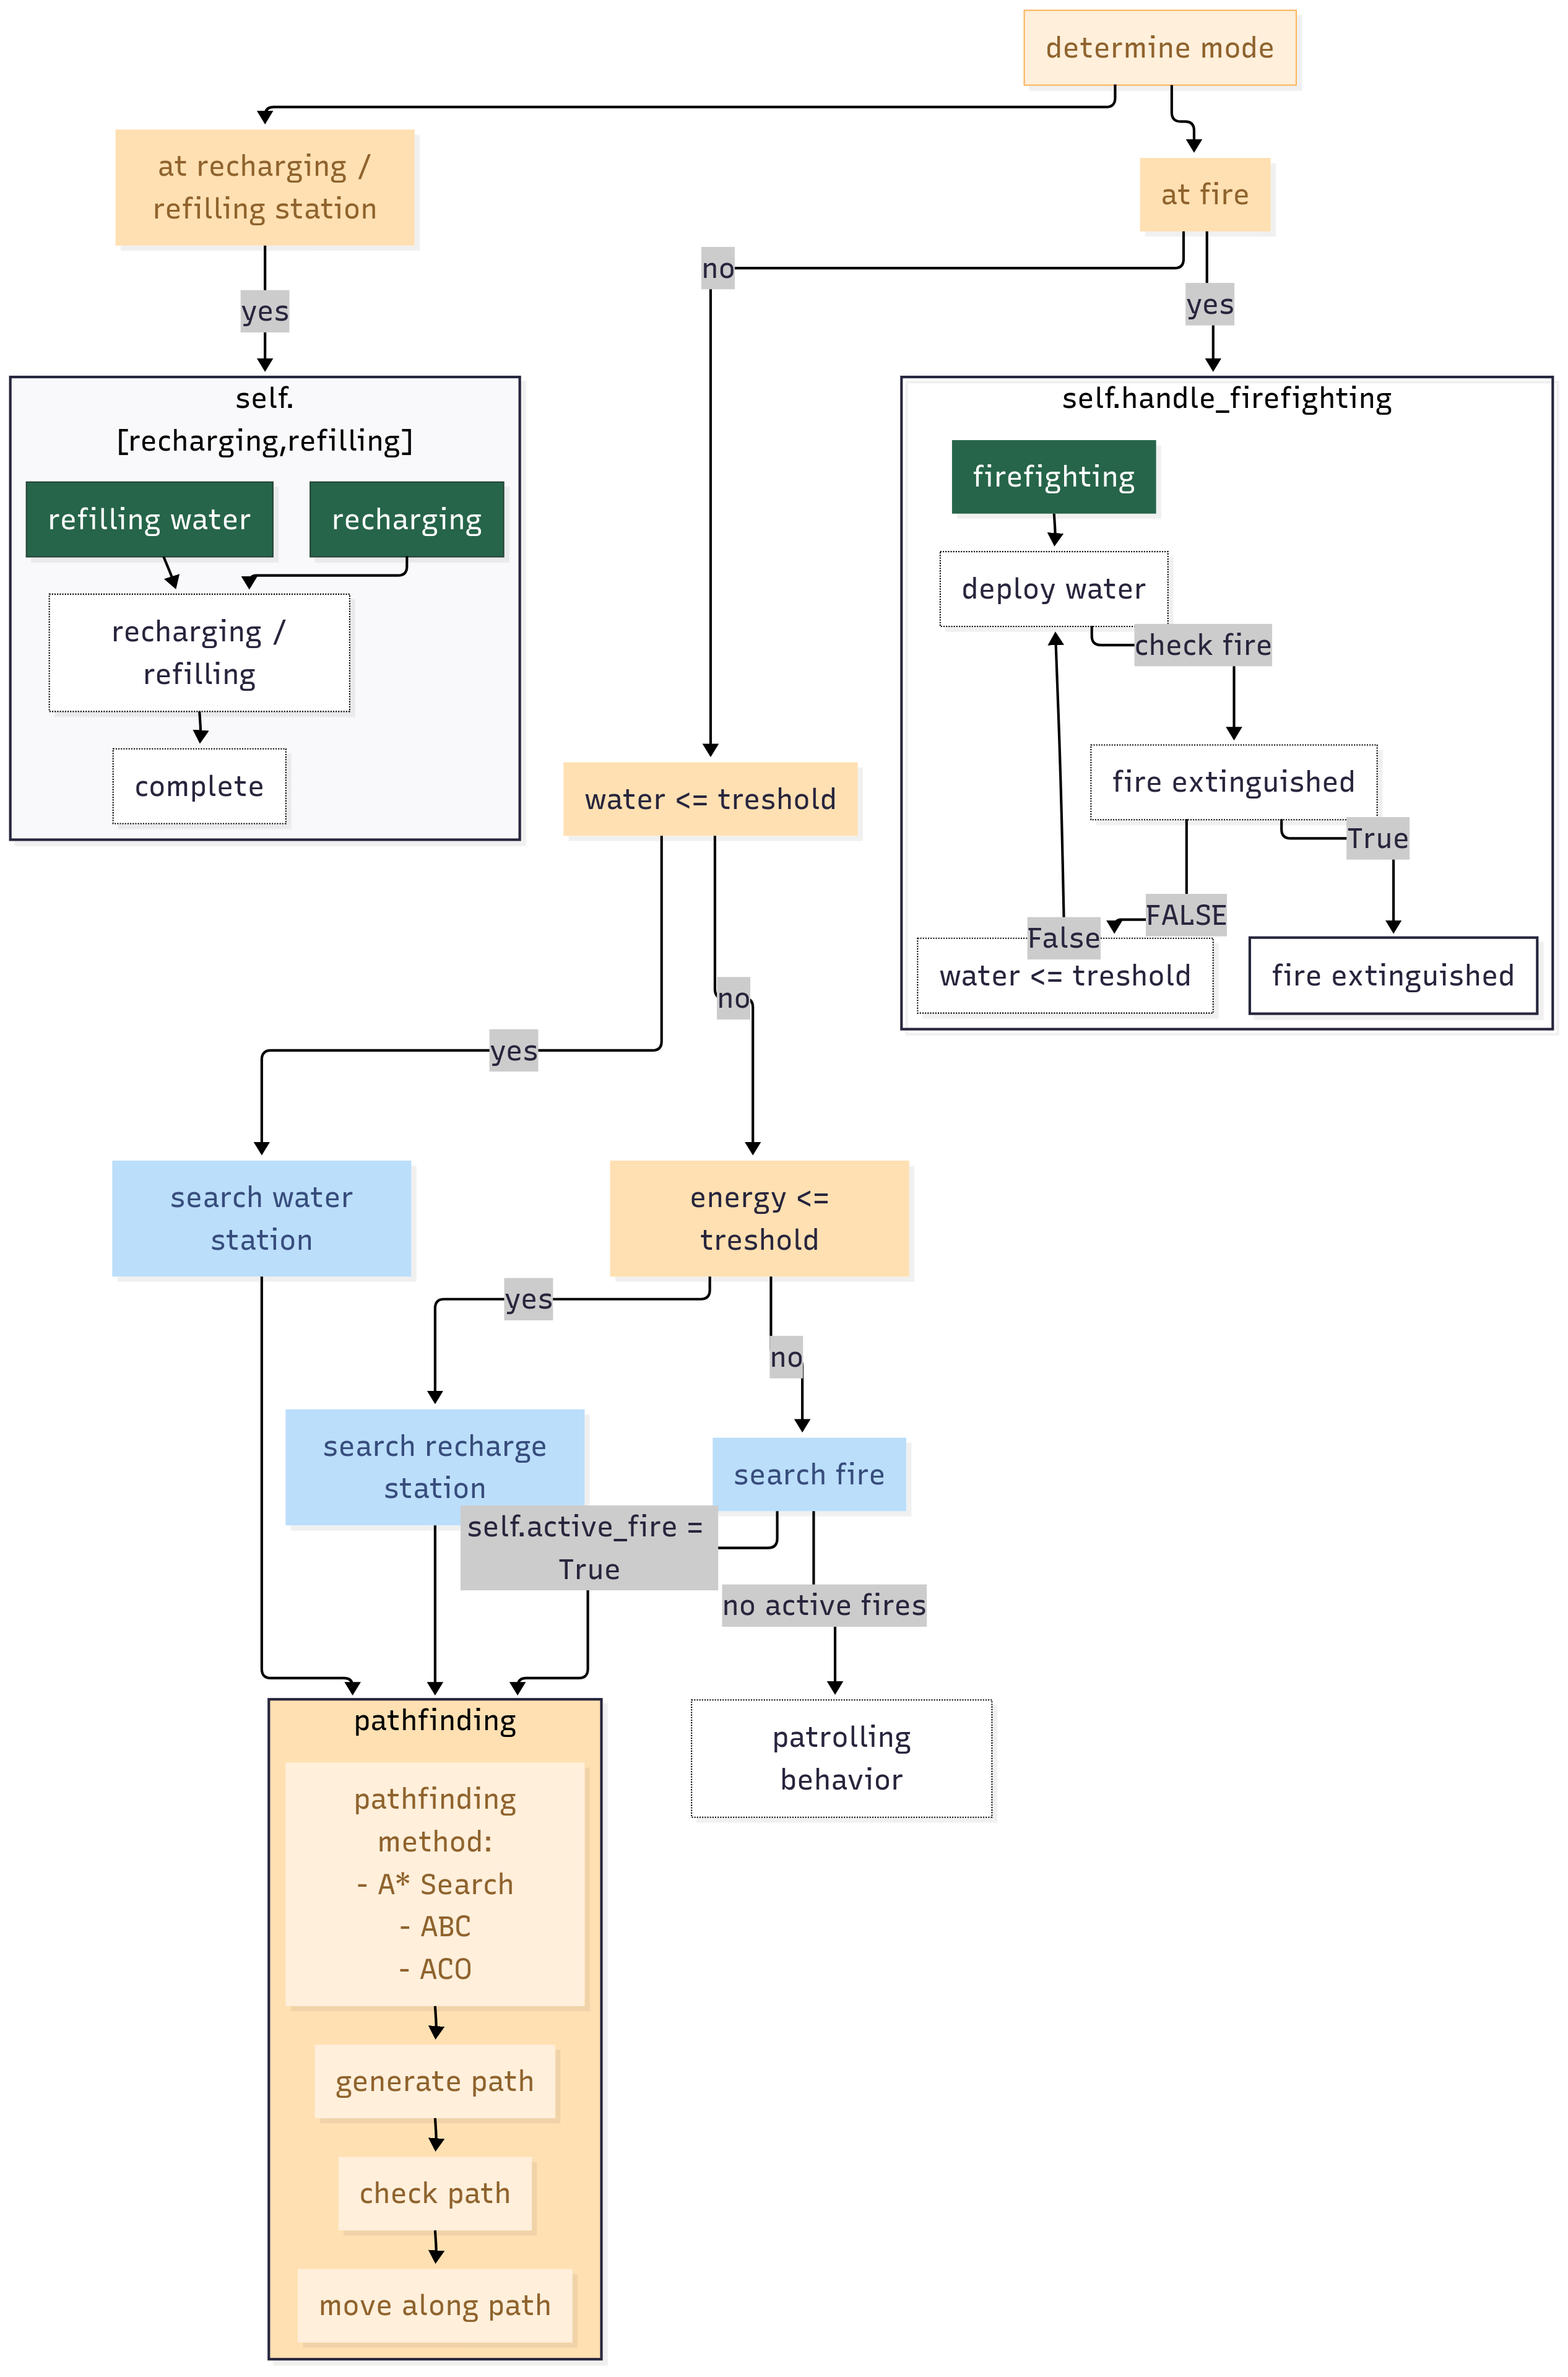
\includegraphics[width=1\textwidth]{figures/DroneAgent_Logic.png}
  \caption{Flowchart of the drone agent’s decision-making process}
  \label{fig:droneAgentlogic}
\end{figure}

\newpage
\subsubsection{Firefighting Plane}
\label{sec:PlaneAgent}

The simulation framework incorporates manned aircraft as a benchmark to evaluate drone-based firefighting solutions. The Lockheed Martin C-130 Hercules was chosen as the reference platform due to its proven operational history, widespread use in aerial firefighting, and well-documented performance characteristics \citep{LockheedC130Hercules2022}. As a repurposed military transport aircraft, the C-130 represents a conventional approach to wildfire management, providing a solid baseline for assessing the effectiveness of emerging drone-based strategies (RQ2). Due to its military design heritage, it offers the capability to carry heavy payloads and has proven itself in reliability.
The C-130 aircraft, used as a reference for the firefighting plane, has an estimated range of \SI{2047}{\nauticalmile} = \SI{3791}{\kilo\meter} with max payload and \SI{4522}{\nauticalmile} = \SI{8375}{\kilo\meter} with an empty payload \citep{LockheedC130Hercules2022}. Considering simplicity, the simulation assumes an average range of \SI{6000}{\kilo\meter} given the fact that the plane is full and empty based on whether the water was dropped or is being delivered to the fire site. Considering these metrics, a fuel consumption of \SI{6}{\liter}/km is calculated.
\[
\text{Fuel Consumption per km} =\frac{36000~\text{L}}{6000~\text{km}} = 6~\text{L/km}
\]

Given a drone speed of 1 field per step, which accounts for 36 km/h \citep{DJIAGRAST50} (equivalent to 10~m/s). Therefore, the speed of the plane needs to be normalized. In comparison, the C-130 has a cruising speed of 600 ~km/h \citep{LockheedC130Hercules2022} (or 167~m/s), considering that the speed for firefighting is significantly lower, a speed of 250~km/h \ (\(\approx 69.4~\text{m/s}\)) is chosen, resulting in a relative speed factor of:

\begin{equation}
\text{Speed Factor}= \frac{70~\text{m/s}}{10~\text{m/s}} = 7
\end{equation}

Therefore, the speed of the plane is defined by the value 7 (positions per step)
This factor is used to scale operational parameters when comparing drone and plane behavior within the simulation. To calculate the fuel consumption with a speed of 250~\text{km/h} \ (\(\approx 69.4~\text{m/s}\)), and simulation steps defined as 1-second intervals:

\[
\text{Fuel Consumption per Step}= (6~\text{L/km}) \times \frac{250}{3600}~\text{km/s} = 0.417\text{ L/step}
\]

The emission rate of the firefighting plane is based on data from \citet*{spicerRapidMeasurementEmissions2009}, which reports an emission of approximately \SI{0.3073}{\kilo\gram} CO\textsubscript{2} for every kilogram of fuel consumed assuming Jet-A fuel with a density of 0.8~kg/L. The emission per step is calculated as follows: 
\[
\text{Emission per Liter}  = 0.3073~\frac{\text{kg CO}_2}{\text{kg fuel}} \times 0.8~\frac{\text{kg fuel}}{\text{L}} = 0.24584~\frac{\text{kg CO}_2}{\text{L}}
\]

\[
\text{Emissions per Step} = 0.417~\text{L/step} \times 0.24584~\frac{\text{kg CO}_2}{\text{L}} = 0.1025~\text{kg CO}_2
\]

As stated by \citet*{spicerRapidMeasurementEmissions2009} is it important to point out that the emissions fluctuate significantly depending on cruising speed and weather conditions. For simplicity reasons, the emissions per step are a fixed parameter calculated as mentioned.

In addition to similar parameters, the logic of the plane also works differently. A key difference is the plane-specific interaction with the runway class, simulating refueling, takeoff, and landing behavior. A key difference between the plane and drone class is its characteristic behavior; the drone has a smaller turning radius and is able to refuel from the resource stations autonomously, whereas the plane is dependent on a runway in order to refuel water and fuel. In addition, the emissions are expected to be much higher because it runs on fossil fuels and not electricity. However, the plane moves faster and has a higher water loading capacity, which enables it, in theory to extinguish fires faster. 

\subsubsection{Runway Agent}
\label{sec:RunwayClass}
The runway agent is created specifically for the firefighting plane. A plane needs a runway to start, takeoff, and refill fuel and water, contradictory to a drone, which can autonomously refill itself and charge itself through a given station. The runway is implemented to ensure a logical approach to real-world firefighting models. It is kept track of whether the runway is currently occupied to make sure multiple planes do not collide. The parameters of the runway class are explained in Table~\ref{tab:runway_parameters} in the Appendix.

\subsubsection{Fire Agent}
\label{sec:FireAgent}

The fire agent has customizable parameters, which allow for complex interactions with the firefighting vehicles. To mimic the real world, the fire agents spawn in the environment with different intensities and have the possibility to spread to a neighboring cell. The spread fire is its own agent with a slightly lower intensity. Through functions such as \texttt{apply\_water(water\_amount)} the fire agent receives water from the given firefighting agent and extinguishes. When fire spreads to neighboring cells, new fire agents are created, meaning that a higher fire count reflects fire area growth rather than the ignition of new fires. The parameters can be observed in Table~\ref{tab:fire_agent_parameters} in the Appendix.

%TC:ignore
\begin{table}[H]
\centering
\caption{Firefighting Plane Class Parameters}
\label{tab:plane_parameters}
\small
\begin{tabular}{@{}p{2.5cm}p{1.5cm}p{6.5cm}@{}}
\toprule
\textbf{Parameter} & \textbf{Value} & \textbf{Description} \\
\midrule
\multicolumn{3}{l}{\textit{Basic Parameters}} \\
unique\_id & int & Unique identifier for the plane agent \\
typ & ``plane'' & Agent type identifier \\
location & None & Current position of the plane \\
goal & None & Target destination \\
path & [list] & Calculated path to destination \\
speed & 7 & Movement cells per step \\
\midrule
\multicolumn{3}{l}{\textit{Resource Parameters}} \\
water\_capacity & \SI{18184}{\liter} & = 4000 gallons (C-130) \citep{LockheedSuperHercules} \\
water & 2000 & Current water level \\
water\_threshold & 500 & Minimum water level before refill \\
water\_used & 0 & Total water used during operations \\
water\_drop\_rate & \SI{8.328}{\liter}/s & = 2200 gallons/s (C-130) \\
fuel\_capacity & \SI{3600}{\liter} & = 9530 gallons \citep{LockheedC130Hercules2022}\\
fuel & 1000 & Current fuel level \\
fuel\_threshold & 200 & Minimum fuel level before refueling\\
\midrule
\multicolumn{3}{l}{\textit{Time and State Parameters}} \\
refill\_time & 10 & Time steps required to refill water \\
refueling & T/F & Boolean indicating refueling state\\
time\_at\_fire & 0 & Time spent at current fire \\
max\_time\_at\_fire & 2 & Maximum time to spend at a fire \\
\midrule
\multicolumn{3}{l}{\textit{Environmental Impact \& Cost}} \\
emission\_rate & 0.24584 & Kg CO\textsubscript{2} / L fuel \citep{spicerRapidMeasurementEmissions2009} \\ 
total\_emission & 0.0 & Cumulative emissions produced \\
operational\_cost & 0.5 & Base operational cost per step \\
fuel\_cost & 0.1 & Cost per unit of fuel \\
total\_cost & 0.0 & Cumulative operational cost \\
\midrule
\multicolumn{3}{l}{\textit{Target References}} \\
current\_target & None & Current target object (fire, runway, etc.) \\
target\_fire & None & Reference to the specific fire being targeted \\
fires & [list] & List of all known fires \\
firefighting & T/F & Boolean indicating firefighting state \\
\bottomrule
\end{tabular}
\end{table}
%TC:endignore



\begin{figure}[htbp]
    \centering
    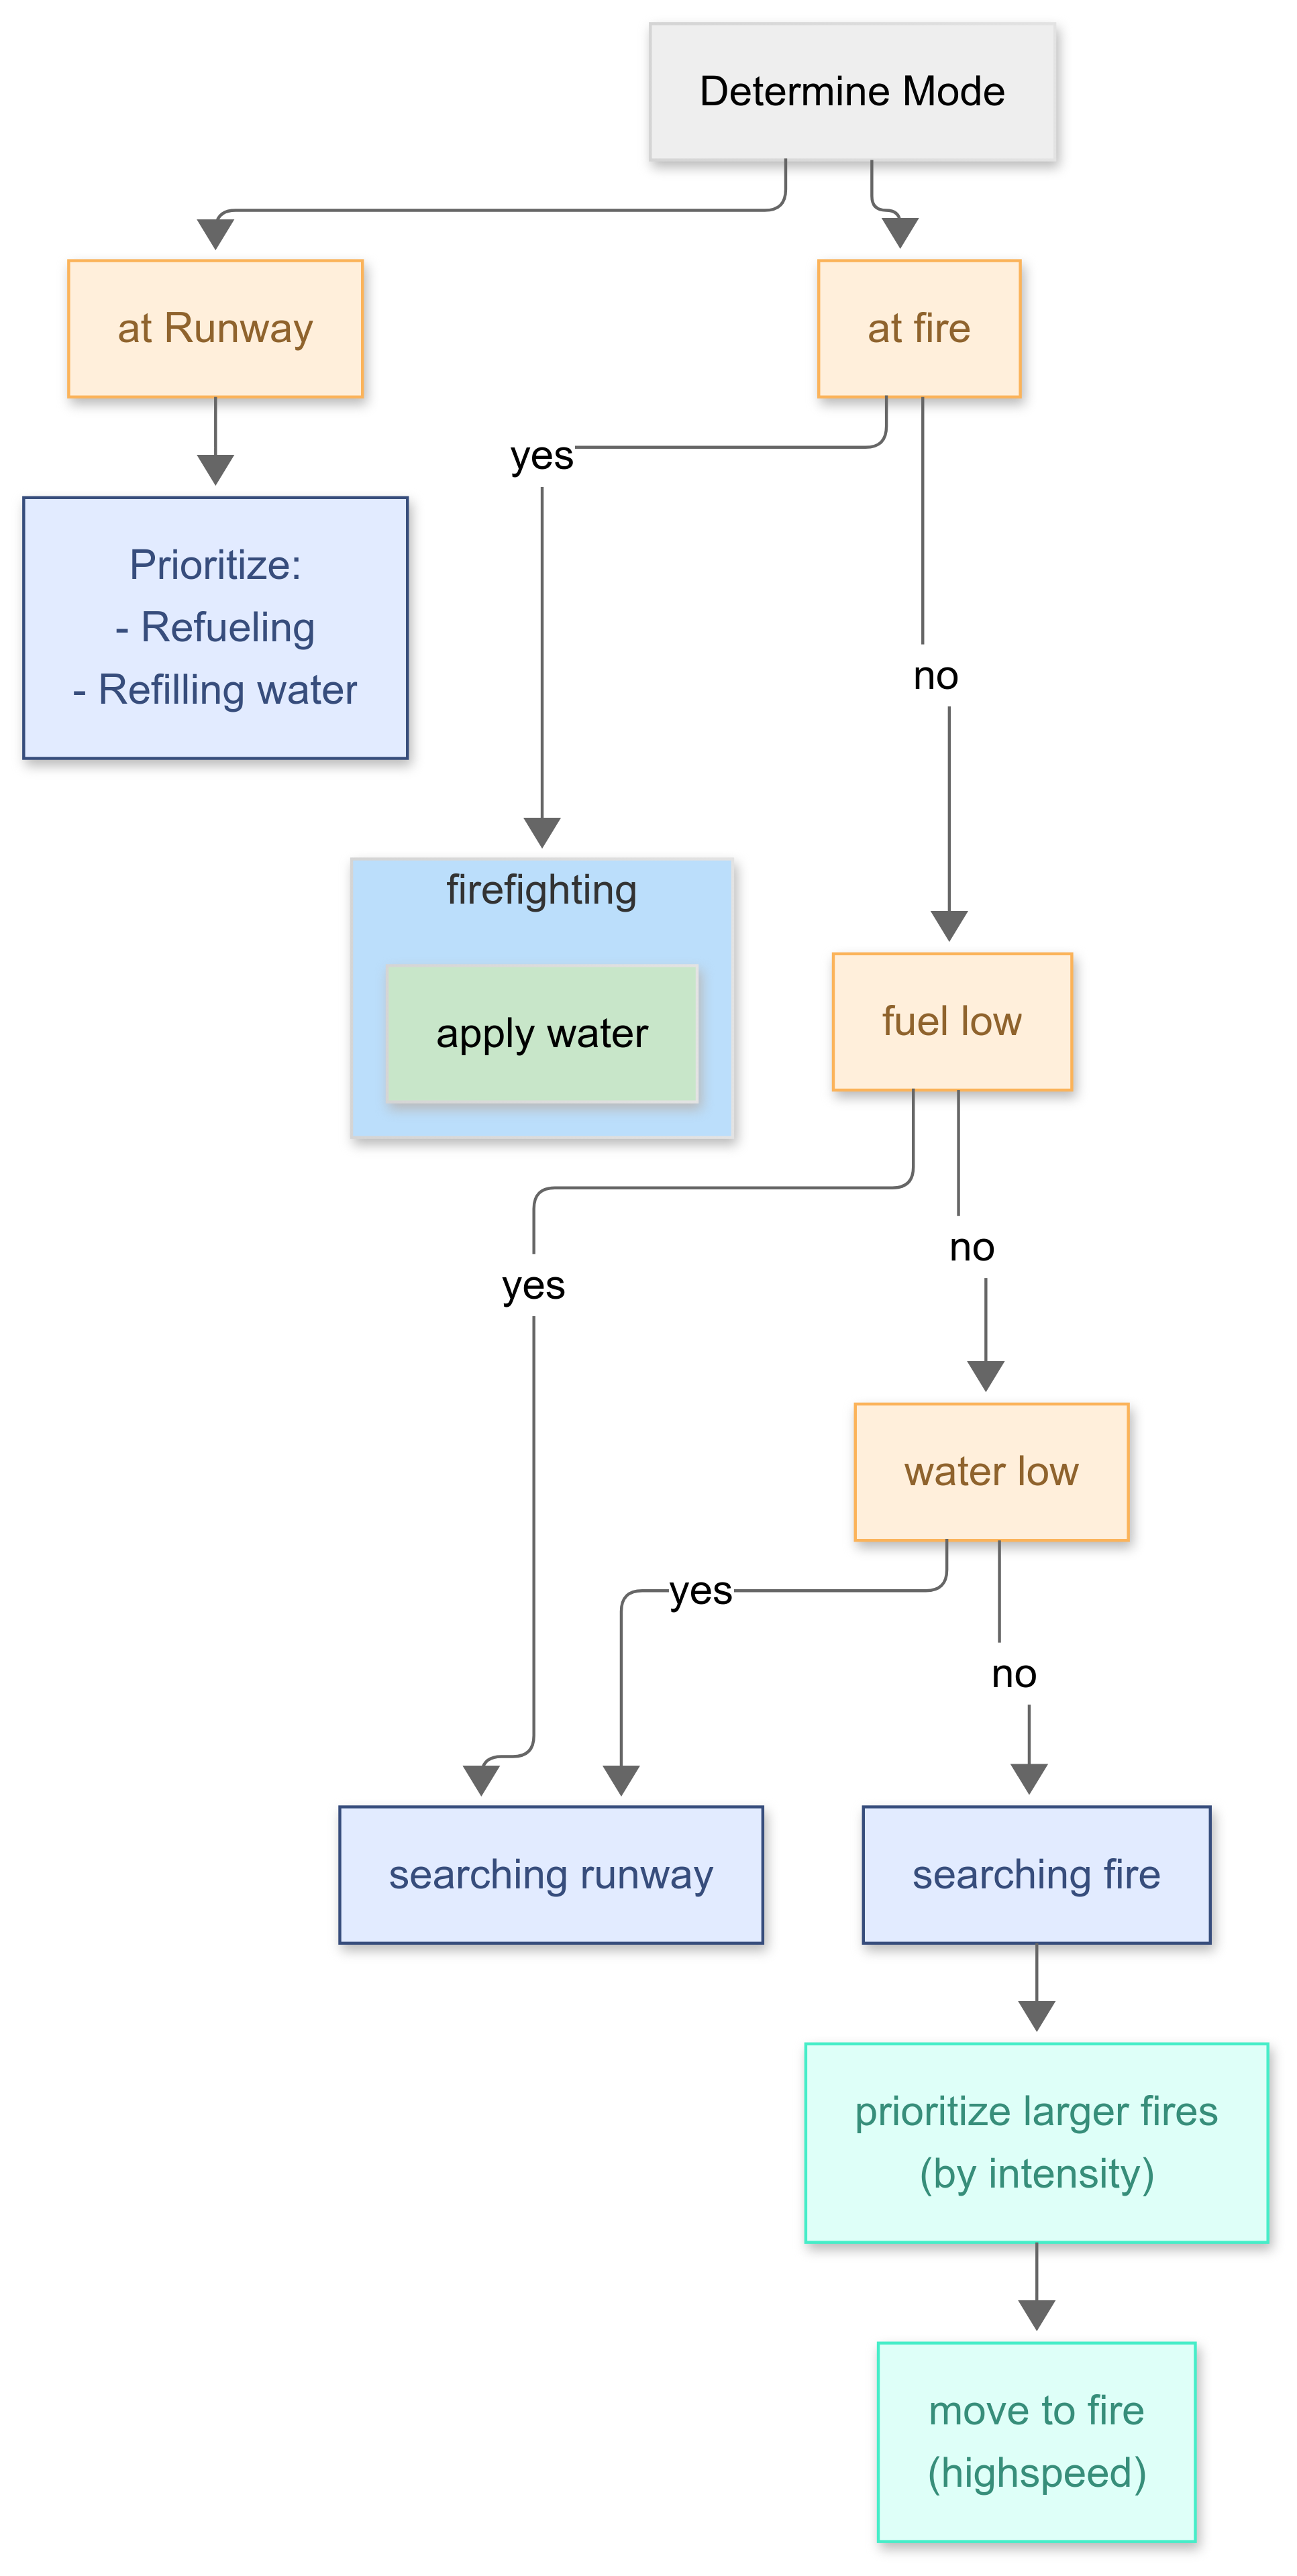
\includegraphics[width=0.8\linewidth]{figures/plane_logic.png}
    \caption{Flowchart of the plane agent’s decision-making process}
    \label{fig:planeLogic}
\end{figure}
\newpage
%TC:endignore


\subsection{Path-finding Algorithms}
Each drone selects paths using one of the following algorithms:
\begin{enumerate}
    \item A* Search: Heuristic-based algorithm with low resource usage. Efficient for small or structured environments. Implemented through the \texttt{heapq} Python library \citep{python-heapq}.
    \item Artificial Bee Colony (ABC): Swarm-inspired, decentralized optimization method effective in dynamic or noisy spaces \citep{karaboga2007abc}.
    \item Ant Colony Optimization (ACO): Probabilistic method using pheromone trails to discover optimal paths over time \citep{ACO}.
\end{enumerate}

The same algorithm is used for all drones within a simulation run to ensure internal consistency. All algorithms are tested across otherwise identical parameters to evaluate comparative performance. These were selected based on experimentation and prior research.

\subsection{Data-Collection}

The simulation is created with the SAT model in mind. Therefore, robust and extensive data collection is needed. At every step every agent's properties are stored in the \texttt{agent\_data} dataframe and the model's properties in the \texttt{model\_data} data-frame. This data collection is enabled through the \texttt{mesa.datacollection.DataCollector{}} which is part of the Mesa framework. \texttt{agent\_reporters} and \texttt{model\_reporters} make this function possible. Extensive details can be found in the \href{https://github.com/kaispeidel/Autonomous-Drone-Firefighting-Simulation}{GitHub repository}.

\subsection{Risk Assessment with Machine Learning}
\label{Risk Assessment with Machine Learning}

To address the main research question of how agent-based modeling can be used to evaluate and optimize autonomous aerial wildfire suppression strategies, two unsupervised learning methods, DBSCAN and K-Means, were implemented for exploratory analysis. This analysis aims to investigate whether simulation outputs contain meaningful patterns that could support more advanced analysis and agent decision-making in future research, rather than direct comparisons between suppression approaches.
\begin{enumerate}
    \item DBSCAN \citep{dbscan}: A density-based clustering algorithm to identify spatial risk zone and corrdination patterns.
    \item K-Means \citep{kmeans}: A centroid-based algorithm to segment environments based on fire intensity and suppression delay.
\end{enumerate}

This exploratory machine learning clustering analysis serves as a proof-of-concept, demonstrating that the ABM framework generates informative emergent patterns, which can be used for further investigation. These algorithms were applied to simulation data capturing fire intensity, suppression history, and spatial coordinates. The main algorithm used was DBSCAN, with falling back to K-Means if DBSCAN failed to converge. Default \texttt{scikit-learn} parameters were used \citep{scikit-learn}, with basic preprocessing (normalization and NaN filtering). The clustering results are presented as a foundation for future research where risk assessment is used as a tool to guide agent behavior. 

\subsection{Technical Implementation and Reproducibility}
\label{Technical Implementation and Reproducibility}
\begin{table}[htbp]
\small
\centering
\caption{Technical Implementation Details}
\label{tab:technical_implementation}
\begin{tabular}{@{}ll@{}}
\toprule
\textbf{Component} & \textbf{Details} \\
\midrule
Language & Python 3.11 \citep{python3.11} \\
\midrule
\multirow{6}{*}{Key Packages} & Mesa \citep{terMesa} \\
& NumPy \citep{numpy} \\
& Pandas \citep{reback2020pandas} \\
& Matplotlib \citep{Matplotlib} \\
& Seaborn \citep{seaborn} \\
& Scikit-learn \citep{scikit-learn} \\
\midrule
Dependencies & Complete list in requirements.txt \\
\midrule
Repository & \href{https://github.com/kaispeidel/thesis}{GitHub Repository} \citep{AgentBasedFirefightingModel_repository} \\
\bottomrule
\end{tabular}
\end{table}
The entire simulation is designed to be reproducible and configurable. All agent parameters, environment size, and algorithm settings can be controlled via parameters.

\subsection{Expected Outcomes and Performance Metrics}
\label{Expected Outcomes and Performance Metrics}
Based on the research questions and experimental setup, this research evaluates the different approaches using the metrics described in Table~\ref{tab:performance_metrics}

\begin{table}[h!]
\centering
\begin{tabular}{lp{7cm}}
\hline
\textbf{Metric} & \textbf{Definition}\\
\midrule
Effectiveness & Time steps required until successful fire suppression (Section~\ref{sec:supression_analysis})\\
\hline
Efficiency & Total accumulated operational cost in euros (€) (see Section~\ref{fig:resources_analysisBIG}) \\
\hline
Sustainability & Resource analysis of total CO\textsubscript{2} emissions in (kg) and water consumption in (L) (see Section~\ref{sec:resource})  \\
\hline
Path-finding Performance & Comparative analysis based on effectiveness, efficiency and sustainability across A*, ACO, and ABC algorithms (see Section~\ref{sec:pathfindingRESULTS})\\
\hline
Trade-off Analysis & Scenarios with higher effectiveness (faster suppression) may exhibit lower sustainability (higher emissions/costs). However, the containment of wildfires has the highest priority. \\
\hline
\end{tabular}
\caption{Explanation of performance metrics in relation to the study objectives}
\label{tab:performance_metrics}
\end{table}

Drone swarms are expected to demonstrate superior cost-effectiveness and lower environmental impact with higher coordination complexity, in line with their individual capacity limitations. In contrast, the plane approach is likely to be the least sustainable but most capable at wildfire suppression. Hybrid systems may offer optimal trade-offs between suppression speed and sustainability. The machine learning model analysis is expected to reveal operational patterns that could inform future decision-making strategies. The performance of the path-finding algorithms is expected to reveal that the A* algorithm performs well in structured environments, while ACO and ABC excel in more dynamic environments. These hypotheses are based on the simulation architecture, agent properties, and path-finding behavior.

\section{Results}

The following section presents the simulation outcomes in alignment with the three research sub-questions. First, the influence of different path-finding algorithms on the movement and coordination of drone agents is evaluated (RQ1). This is followed by a comparative analysis of suppression performance across drone-based, plane-only, and hybrid configurations (RQ2). Lastly, trade-offs between suppression effectiveness, operational efficiency, and sustainability—measured through CO\textsubscript{2} emissions, water consumption, and cost-are assessed (RQ3). These results provide a structured basis for understanding how agent-based modeling can be applied to evaluate and optimize autonomous aerial wildfire suppression strategies.

\subsection{Path-Finding}
\label{sec:pathfindingRESULTS}
To address the main research question and RQ2, it is necessary to first present the results addressing RQ1, which investigates the performance of different path-finding algorithms. The simulation provides clear visual evidence that each algorithm employs a distinct movement strategy. In the visualizations, each drone’s path is depicted as a blue line, recharge stations are shown as yellow circles, and water stations as blue circles. Separate figures are dedicated to A*~\ref{fig:a_star}, Ant Colony Optimization (ACO)~\ref{fig:aco} and Artificial Bee Colony (ABC)~\ref{fig:abc}, each illustrating the algorithm’s trajectory under identical initial fire conditions (\texttt{fires\_n = 50}), respecting model complexity considerations ~\ref{sec:computational_complexity}. Each plot is generated after 1000 simulation steps.
It is important to note that results can vary between simulation runs; thus the figures presented here serve as representative examples. Accordingly, it is possible that some fires are still not contained; those are marked as red circles, with the size reflecting their intensity. The same logic applies for extinguished fires, marked as green circles.
The ``active'' label in the plot describes ongoing fires, while the ``total fires'' metric represents the cumulative number of ignited fires throughout the simulation, highlighting that the fire spread mechanic is working properly.

\begin{figure}[htbp]
    \centering
    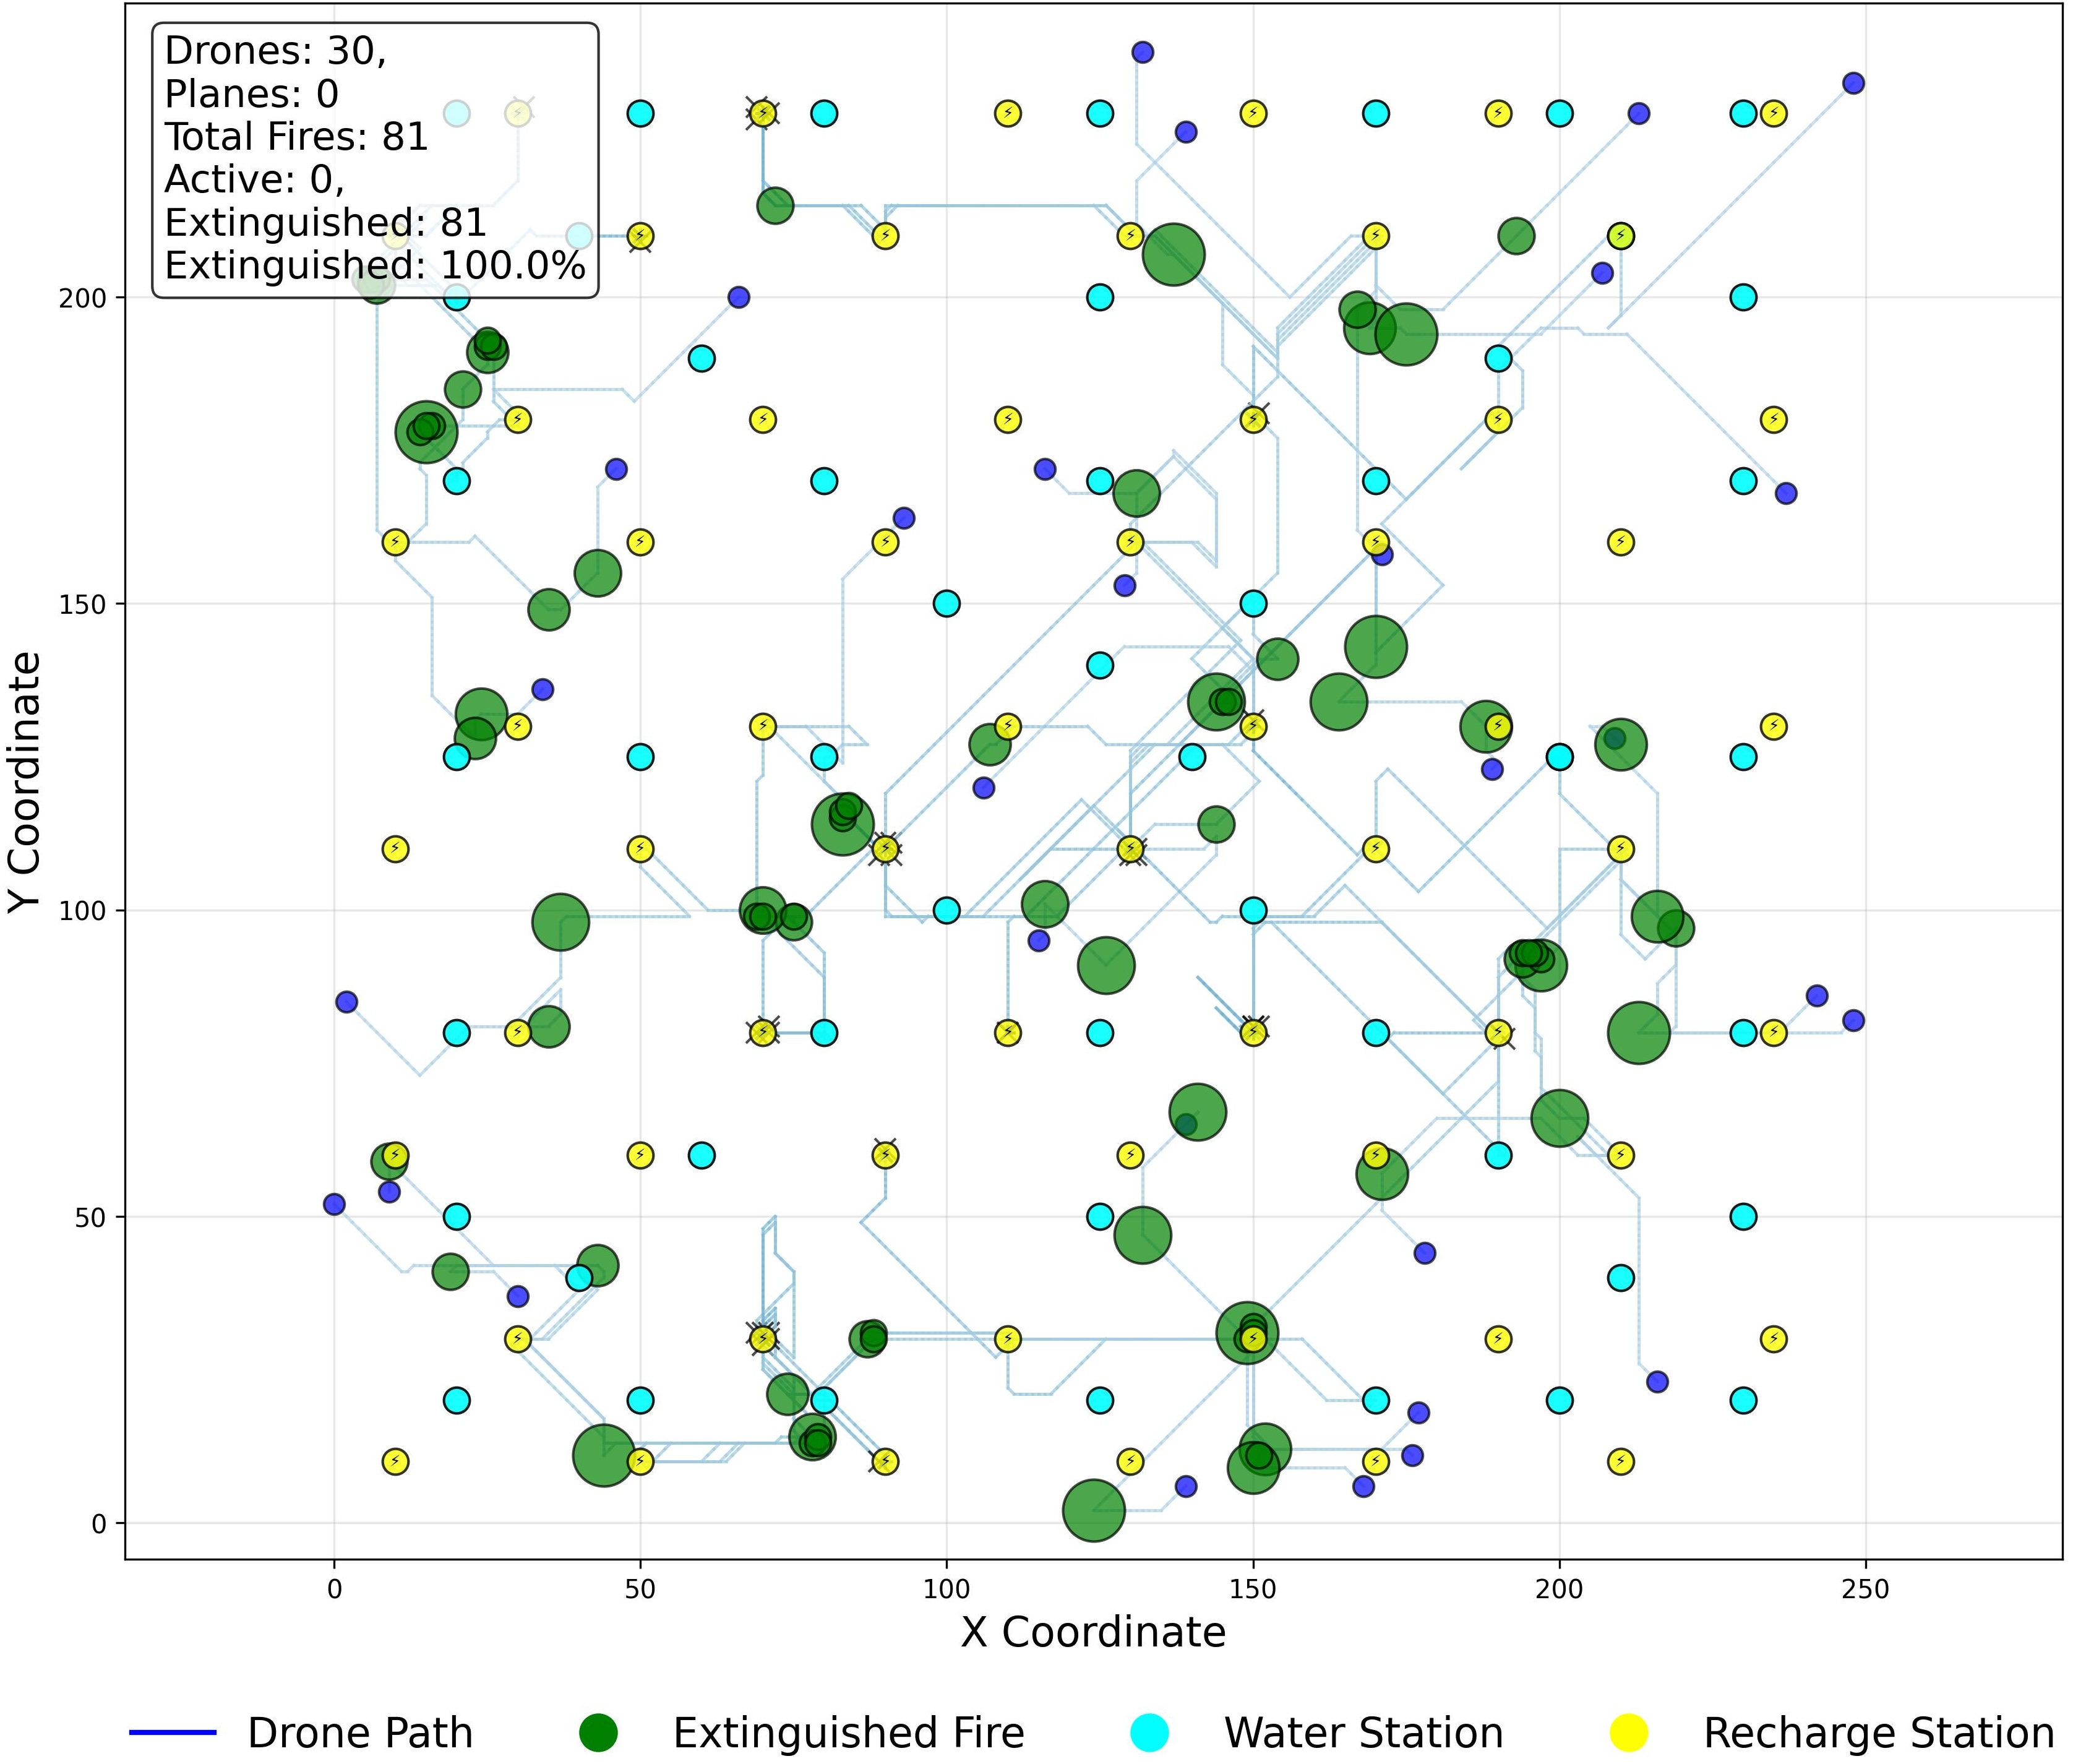
\includegraphics[width=0.9\linewidth]{figures/A*_agent_paths.jpeg}
    \caption{Path trajectories of drone agents using A*}
    \label{fig:a_star}
\end{figure}

Figure~\ref{fig:a_star} the drone-based approach using the A* algorithm, achieving 100\% fire suppression (81 out of 81 fires extinguished), with direct and efficient trajectories and coordinated resource management. In contrast, Figure~\ref{fig:aco} illustrates the ACO algorithm, which exhibits adaptive swarm behavior but only extinguishes 46.4\% of fires within the simulation steps (no convergence). This example was intentionally selected. Accordingly, this visualization provides evidence into the drone's trajectory and suggests that resource station placement or drone allocation should be adjusted in areas where fires grew larger.

\begin{figure}[htbp]
    \centering
    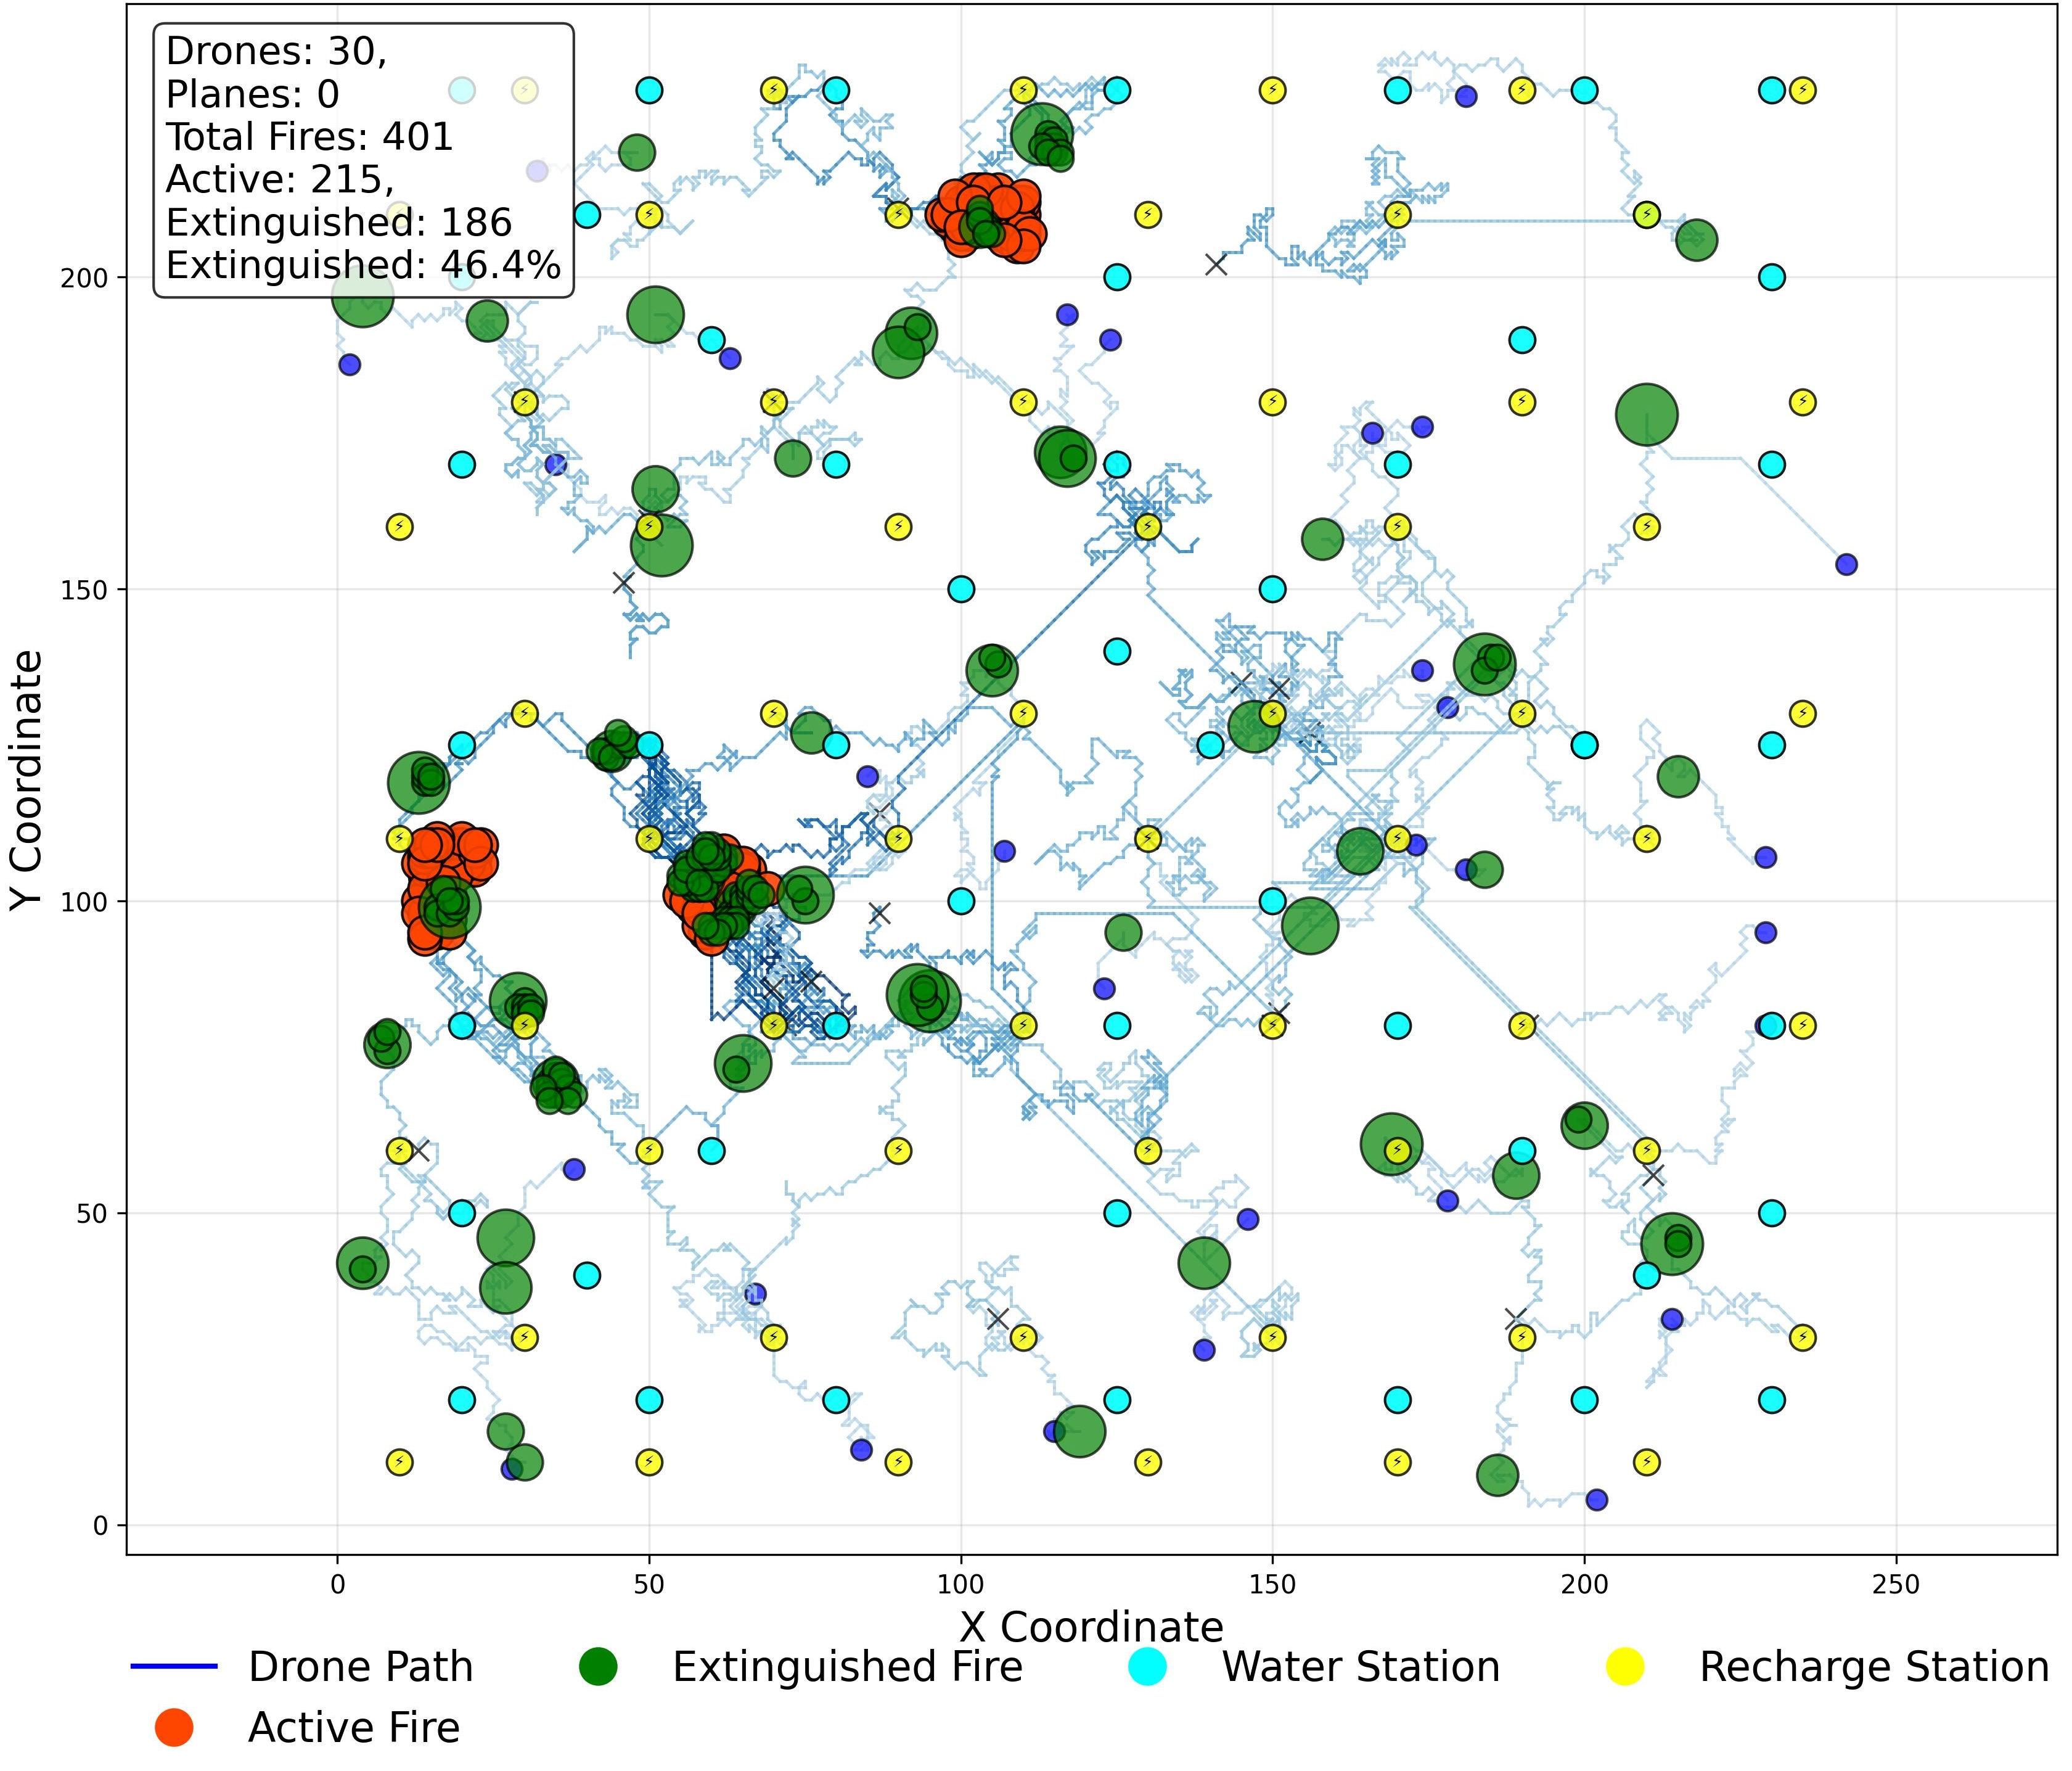
\includegraphics[width=0.9\linewidth]{figures/ACO_agent_paths.jpeg}
    \caption{Path trajectories of drone agents using Ant Colony Optimization}
    \label{fig:aco}
\end{figure}

The trajectory of the ABC algorithm, illustrated in Figure~\ref{fig:abc}, exhibits a similar trajectory behavior but manages to contain 98.5\% of fires. Interestingly, the paths appear less coordinated compared to the A* and ACO approaches. This phenomenon is likely attributable to ABC's initial broad exploration behavior, which uses significant resources, resulting in frequent visits to resource stations, as evidenced by the denser clustering of paths around resource stations. While this intensive exploration strategy may compromise immediate efficiency, it potentially enhances long-term coverage optimization through comprehensive environmental exploration.

\begin{figure}[htbp]
    \centering
    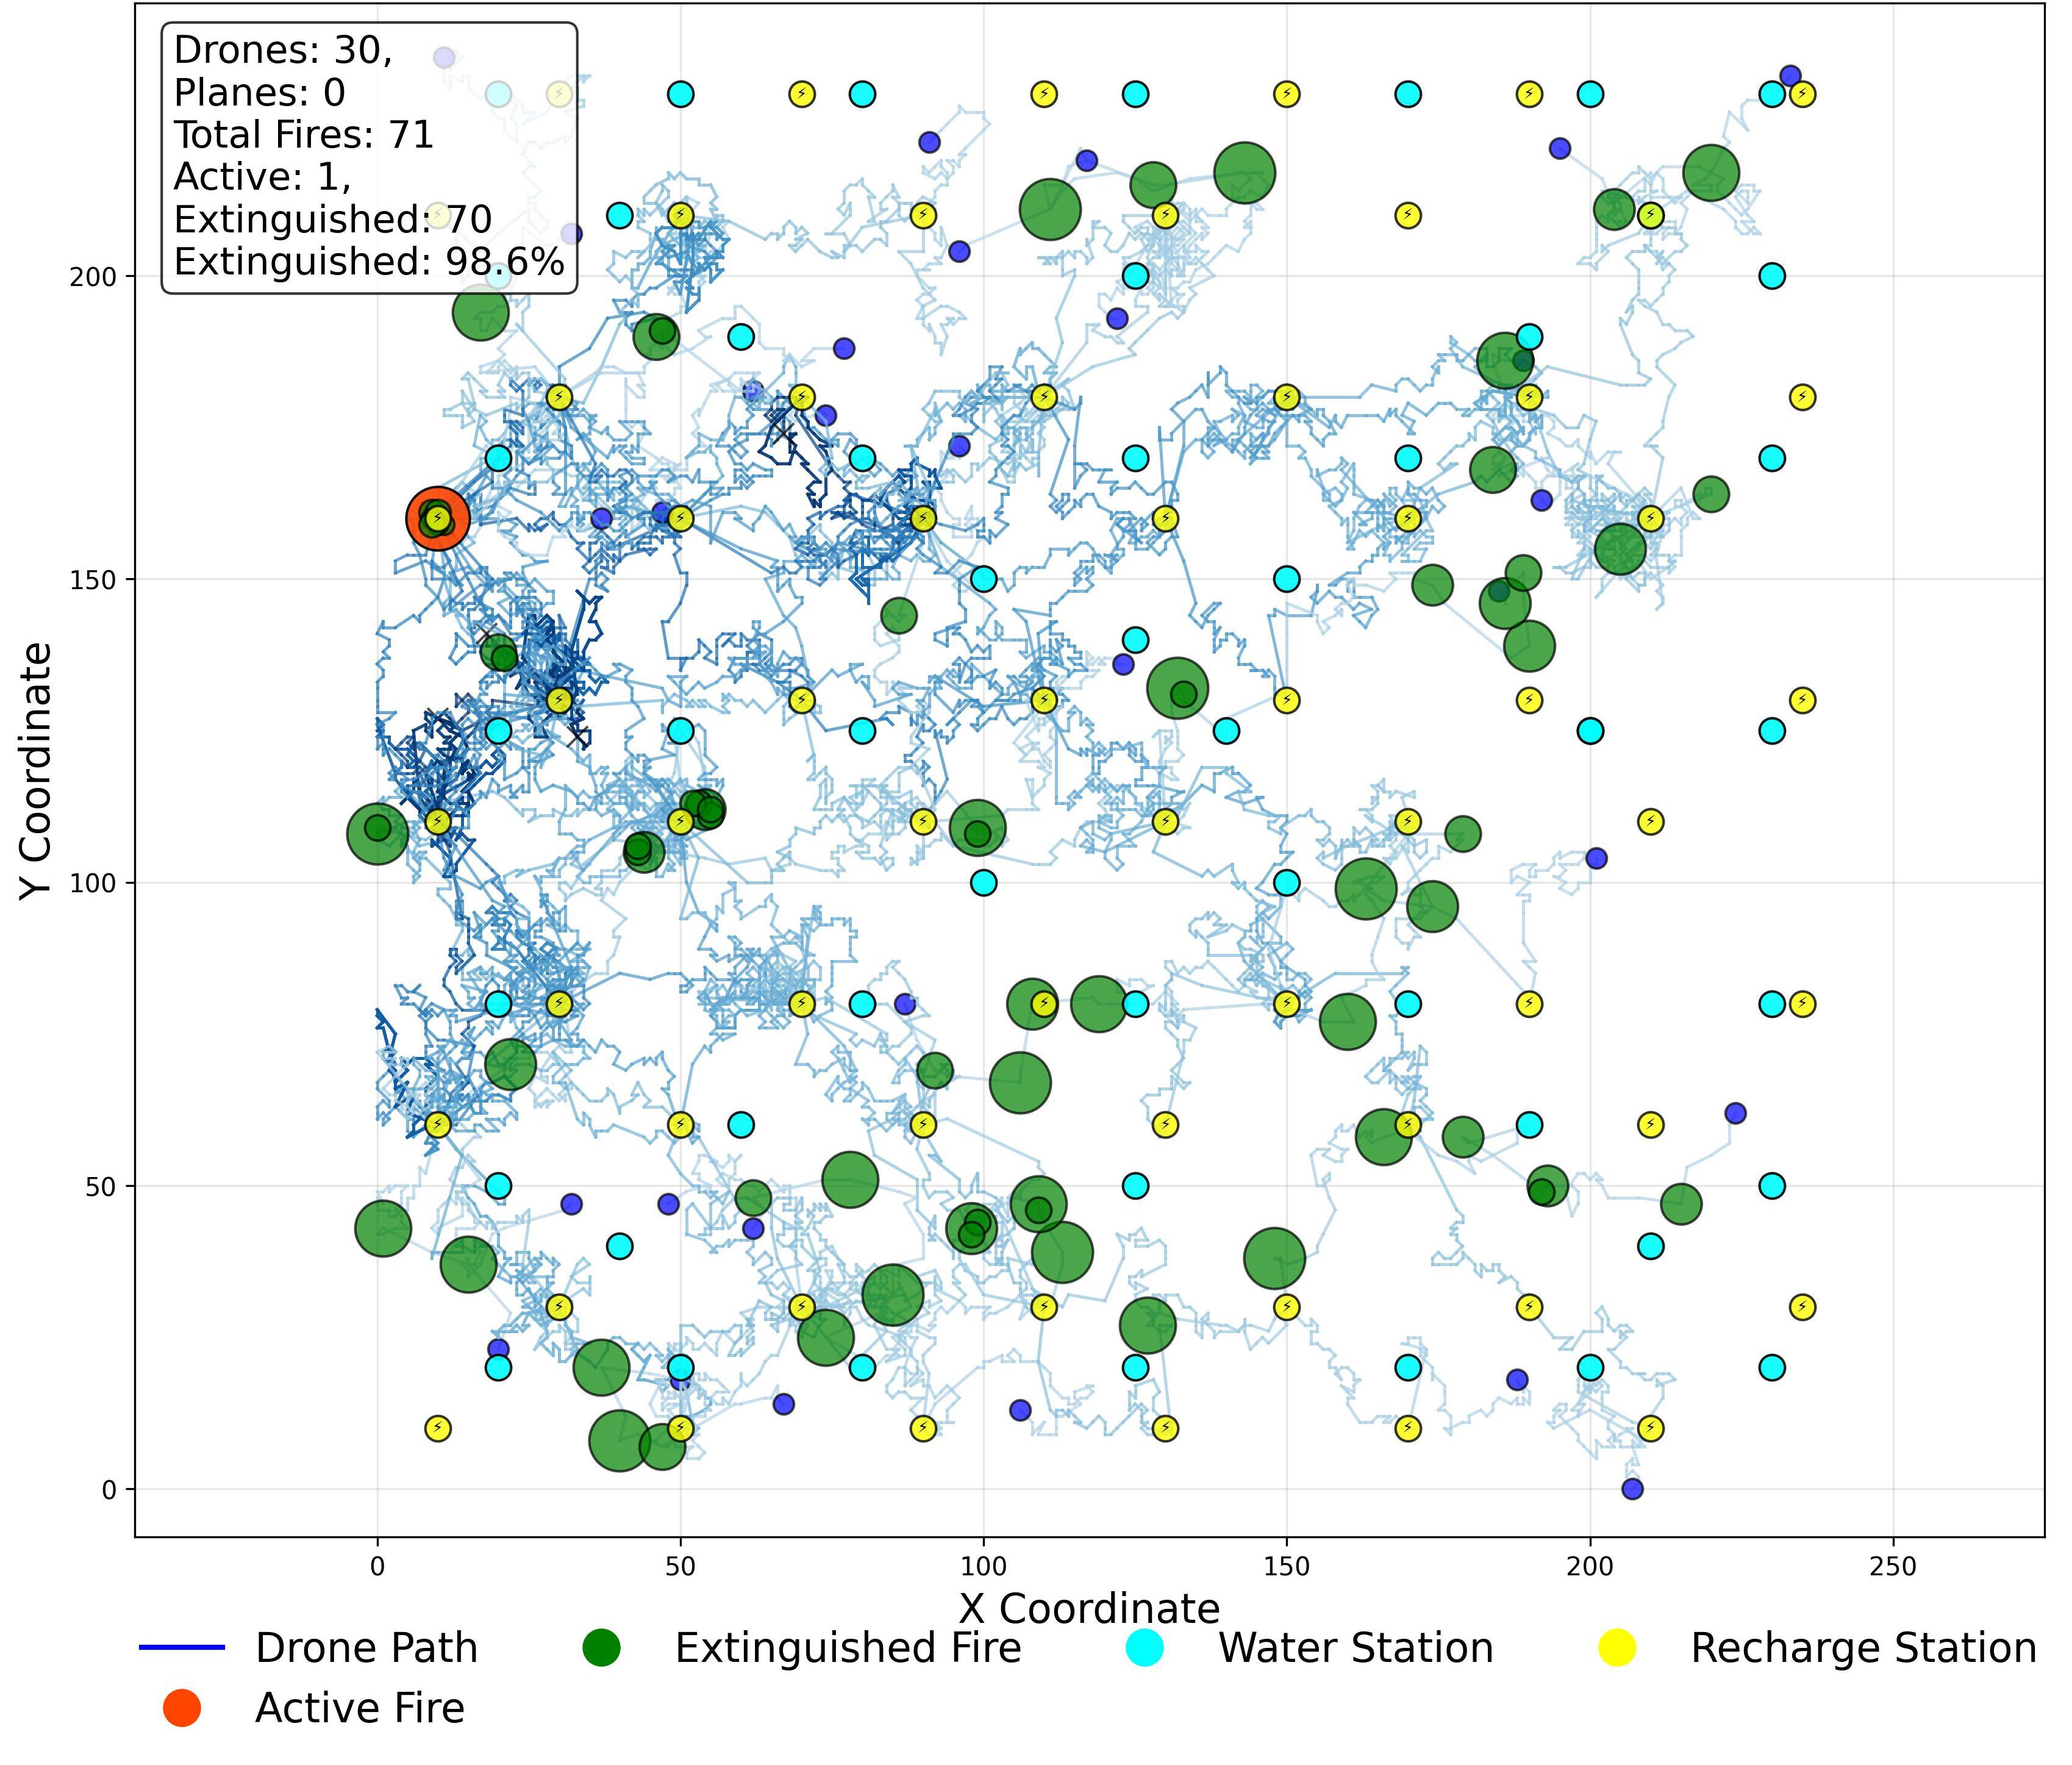
\includegraphics[width=0.9\linewidth]{figures/Artificial_Bee_Colony_agent_paths.jpeg}
    \caption{Path trajectories of drone agents using Artificial Bee Colony}
    \label{fig:abc}
\end{figure}

Drones demonstrate efficient resource management by clustering around resources while maintaining suppression coverage across the 250×250 environment. The high suppression effectiveness with minimal path redundancy supports sustainability, as efficient routing reduces energy consumption and operational costs, directly addressing RQ3. The successful coordination of 30 autonomous agents validates the scalability potential.

Figure~\ref{fig:plane_path} reveals the unique operational characteristics of the aircraft-based approach. The trajectories exhibit mainly linear patterns, constrained by mandatory runway (purple cross) interactions for takeoff, landing, and refueling operations. This infrastructure dependency significantly limits operational flexibility, particularly impacting the suppression of fires located at greater distances from the runway, thus achieving only 52.4\% suppression effectiveness with 258 active fires remaining. The resulting coverage pattern demonstrates clear spatial differences, with reduced effectiveness in peripheral areas of the simulation environment. This emergent behavior clearly demonstrates the trade-off between aircraft capacity and operational flexibility.
In contrast, the hybrid approach exhibits observable patterns suggesting intelligent resource allocation between aircraft and drone technologies. Figure~\ref{fig:hybrid_path} provides evidence of planes handling most suppression tasks, while drones appear to provide supplementary coverage for distant or smaller fires. These behavioral characteristics suggest the potential of collaborative systems, with additional evidence presented in Section~\ref{sec:supression_analysis}.

\begin{figure}[H]
    \centering
    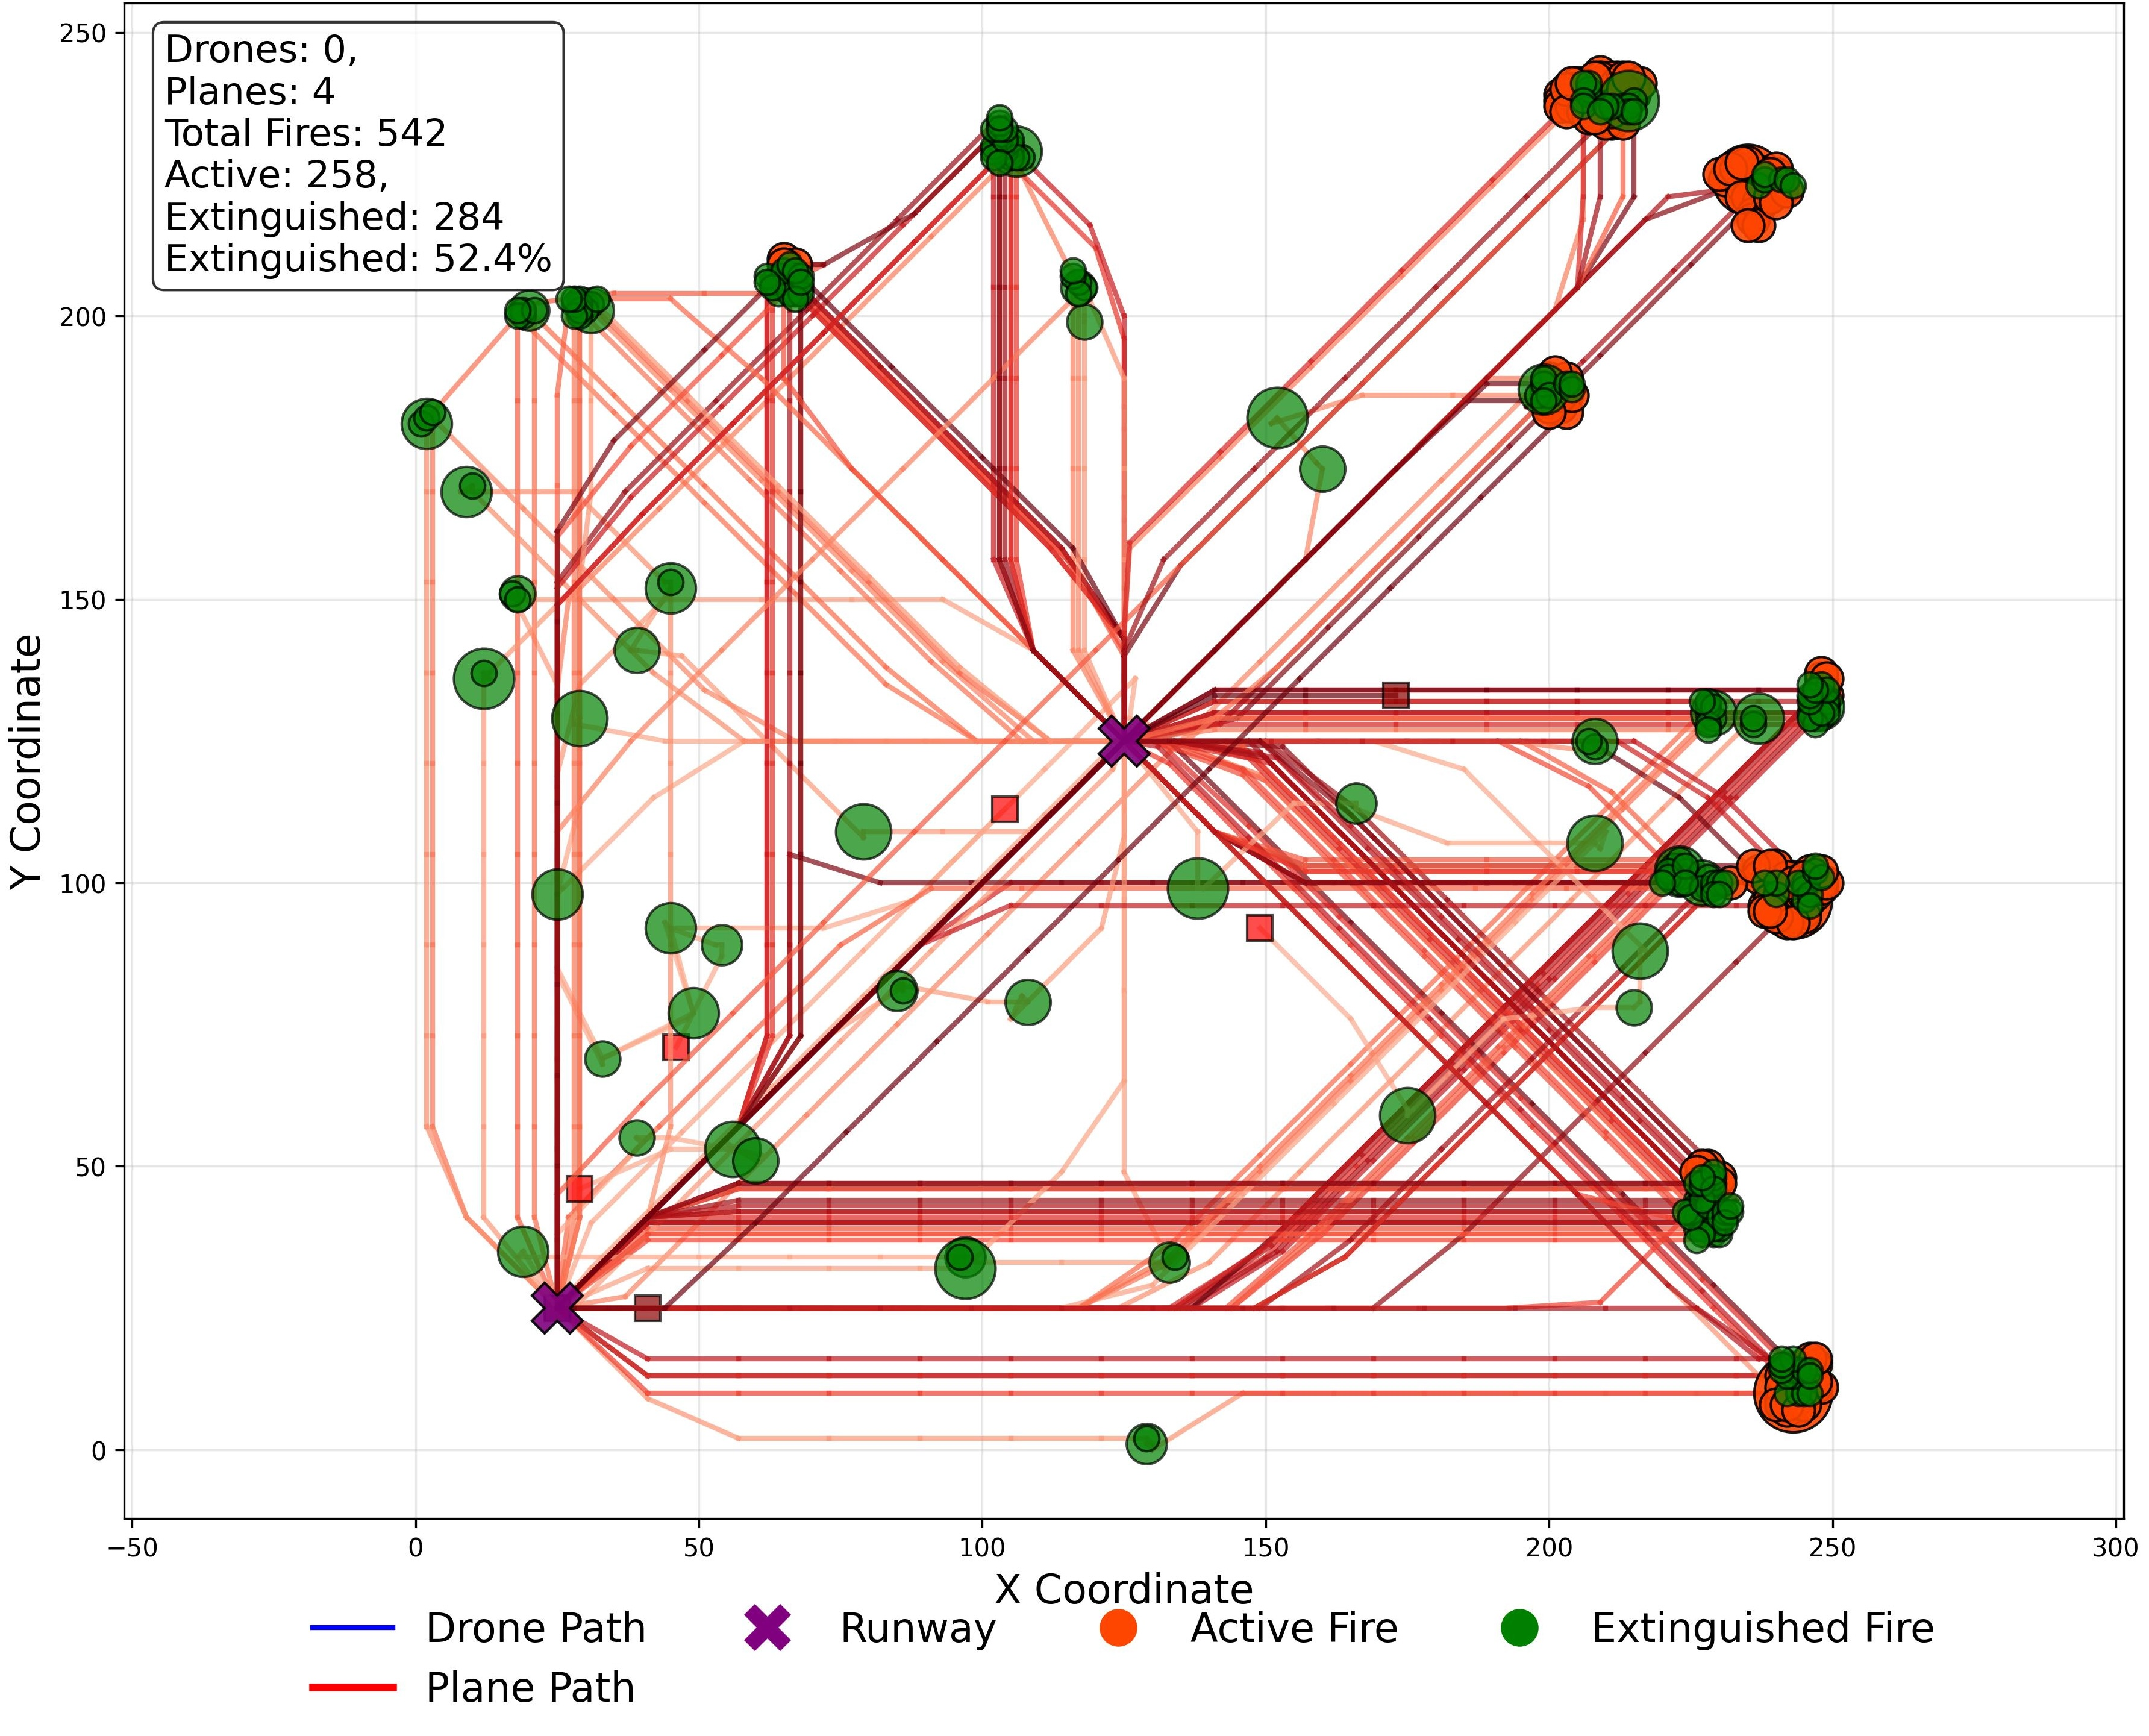
\includegraphics[width=0.9\linewidth]{figures/Firefighting_Plane_agent_paths.jpeg}
    \caption{Path trajectories of aircraft agents}
    \label{fig:plane_path}
\end{figure}

\begin{figure}[H]
    \centering
    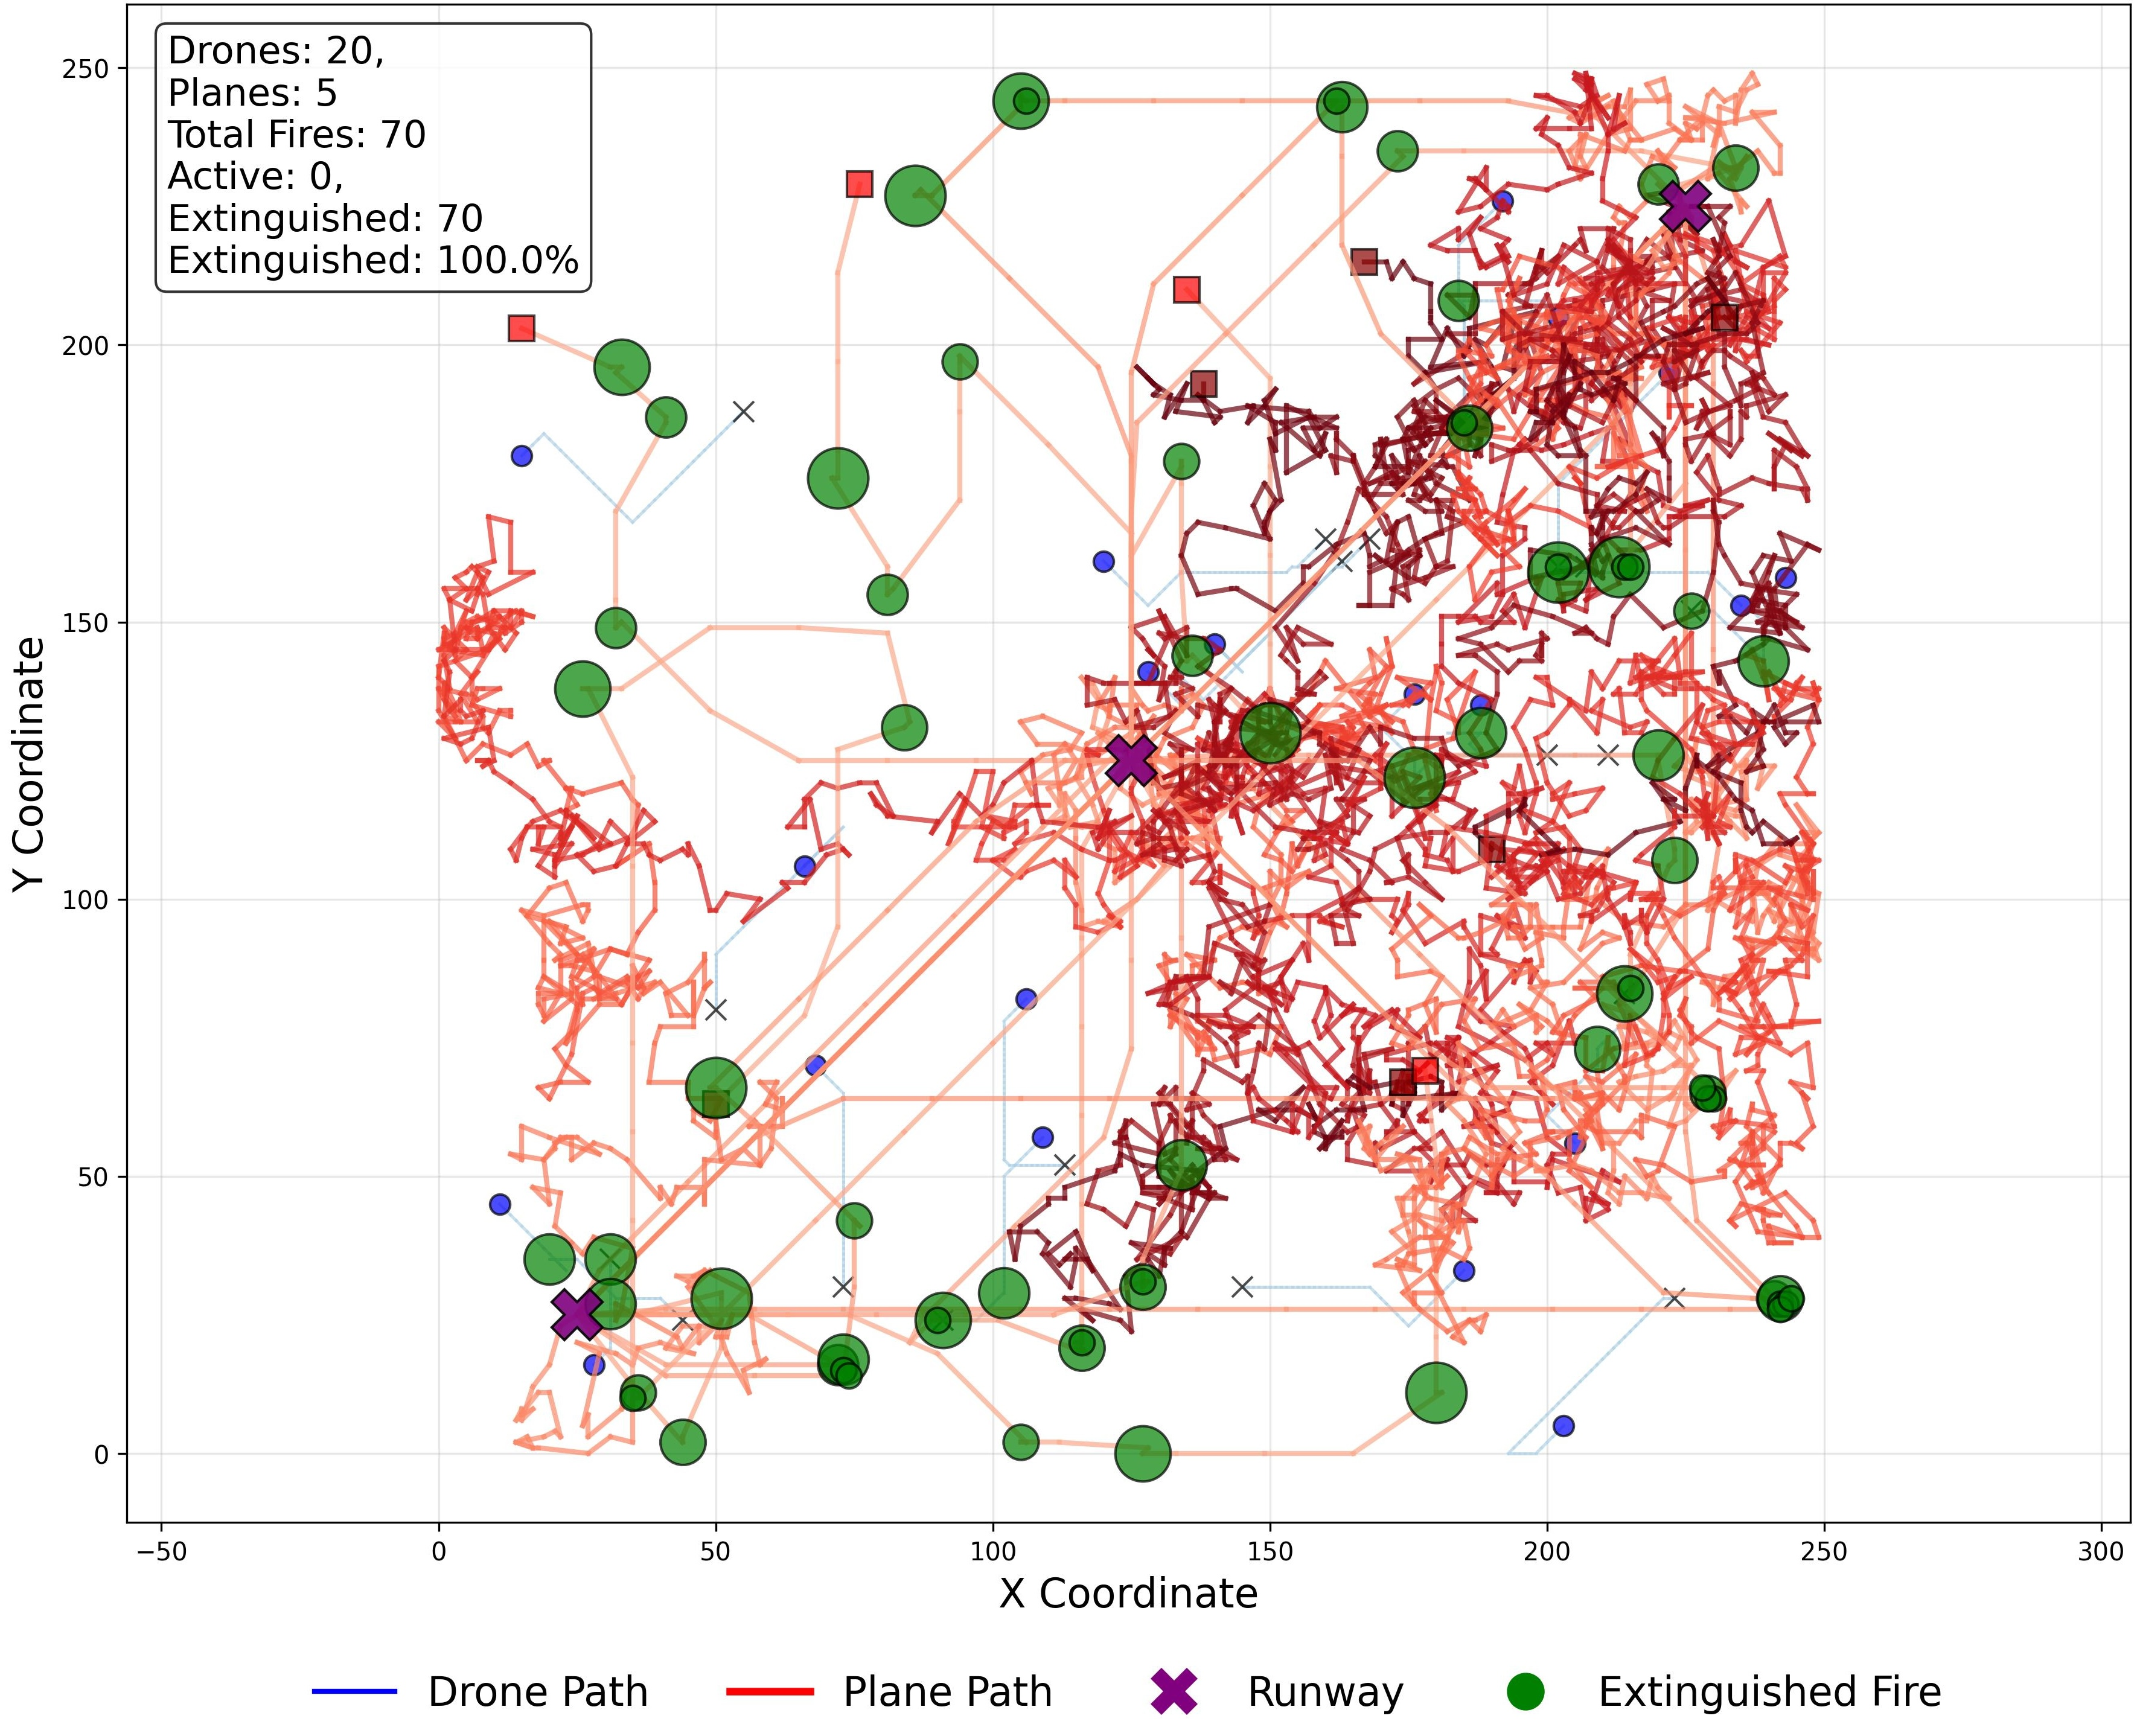
\includegraphics[width=0.9\linewidth]{figures/Hybrid_agent_paths.jpeg}
    \caption{Path trajectories of drone agents and aircraft}
    \label{fig:hybrid_path}
\end{figure}


Collectively, these individual plots address RQ1 and validate the correct integration of all algorithms into the simulation, showcasing how different navigation strategies and swarm behaviors emerge in the defined environment. 


\subsection{Suppression Analysis}
\label{sec:supression_analysis}

To address RQ2, the mean number of active fires at each time step was calculated across 1000 independent simulation runs. Figure~\ref{fig:comparitive_analysislineplot} illustrates these results, with 95\% confidence intervals (CI's) depicted as shaded regions around each suppression line. Wider confidence intervals indicate greater variability and thus lower consistency in suppression performance.
The results show that drone-based approaches (using ABC, A*, and ACO algorithms) and the hybrid approach maintain consistent suppression performance, as indicated by thinner confidence intervals. In contrast, the plane-only approach displays the widest confidence intervals and the greatest variability in the number of active fires throughout the simulations, indicating less consistency in suppression effectiveness.
Overall, these findings suggest that drone-based and hybrid approaches not only achieve similar levels of effectiveness but also provide more consistent results than the plane-only approach. The results also imply that incorporating drones into traditional plane-based suppression strategies could improve consistency and reliability in wildfire management within the context of this simulation study.

\begin{figure}[htbp]
    \centering
    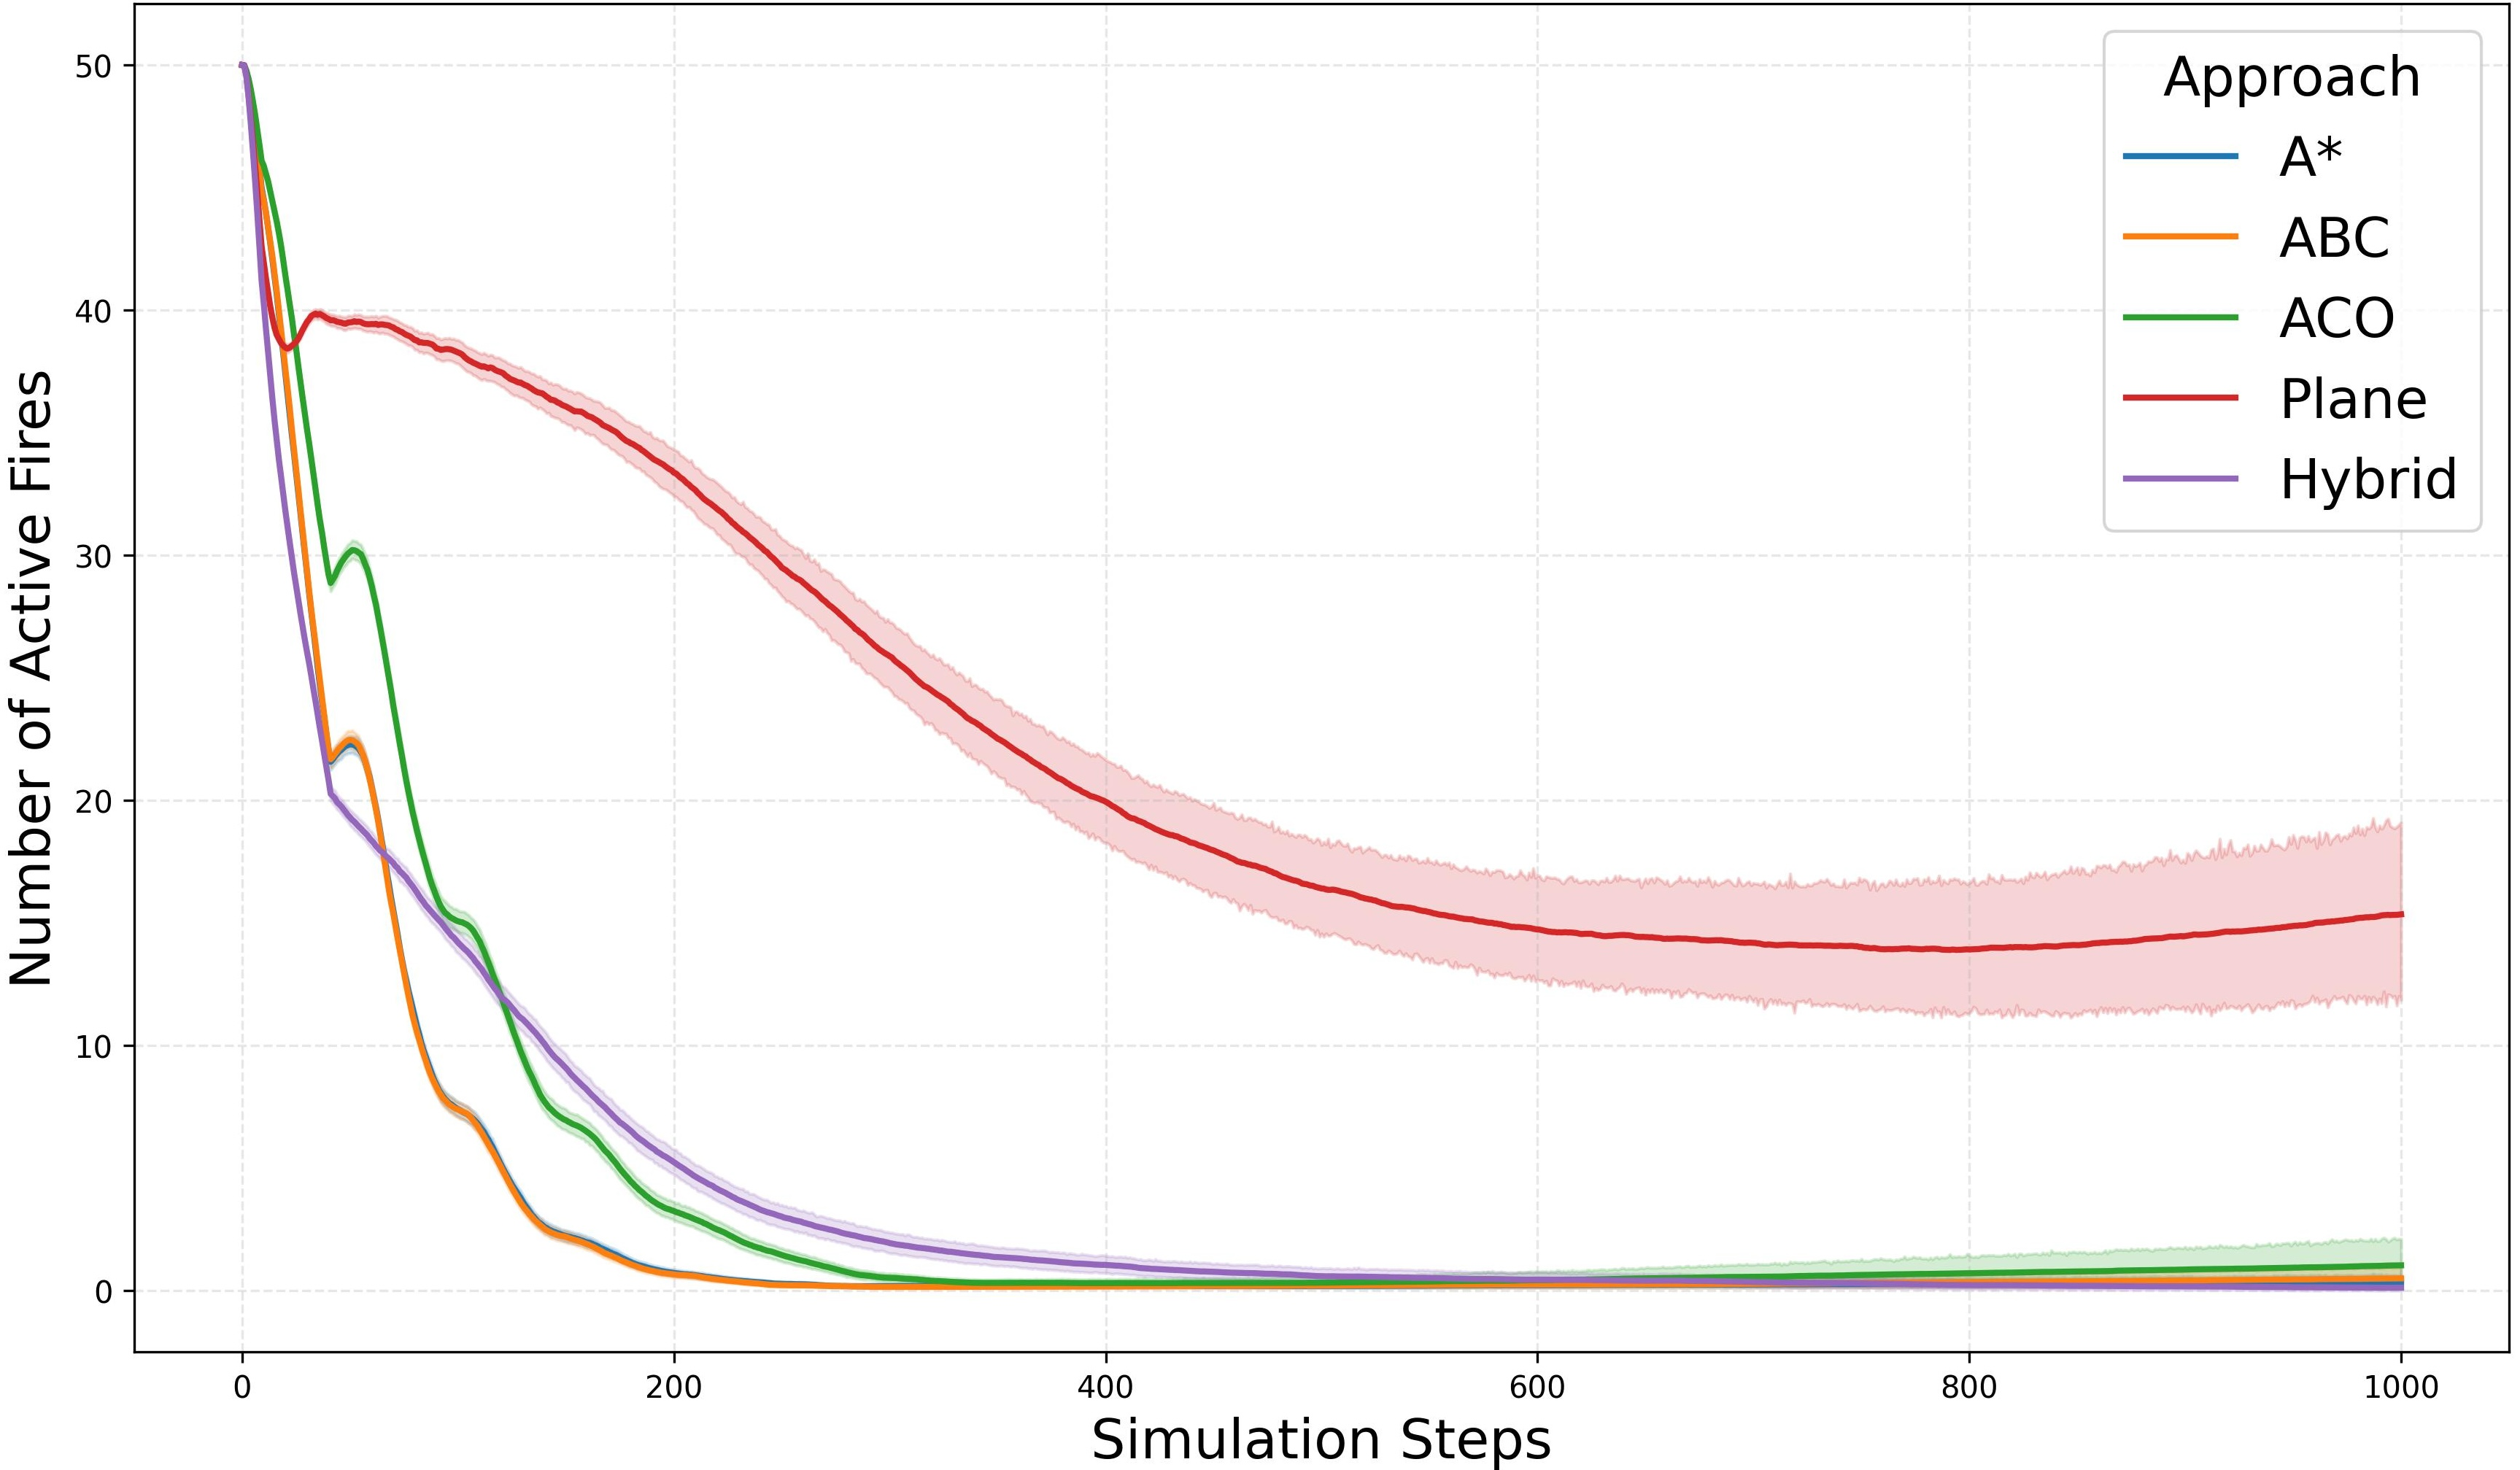
\includegraphics[width=1\linewidth]{figures/fire_progression_analysis.jpeg}
    \caption{Fire progression analysis: active fires across 1,000 simulations with 95\% confidence intervals}
    \label{fig:comparitive_analysislineplot}
\end{figure}

Effectiveness was further assessed by analyzing the number of simulation steps required to achieve complete fire suppression for each approach. Figure~\ref{fig:comparitive_analysis} displays the mean suppression times and associated variability (as standard deviation) for each configuration, with error bars representing a 95\% confidence interval.
The drone-only approaches: ABC (229.3 ± 15.9 steps), A* (237.9 ± 16.2 steps), and ACO (291.6 ± 16.5 steps) consistently outperformed the aircraft-only approach (505.1 ± 14.6 steps), which also regularly failed to converge within the defined runtime. The hybrid approach (drones + aircraft) demonstrated the fastest average suppression time (223.3 ± 7.0 steps) and the lowest variability, indicating both efficiency and reliability.

\begin{figure}[htbp]
    \centering
    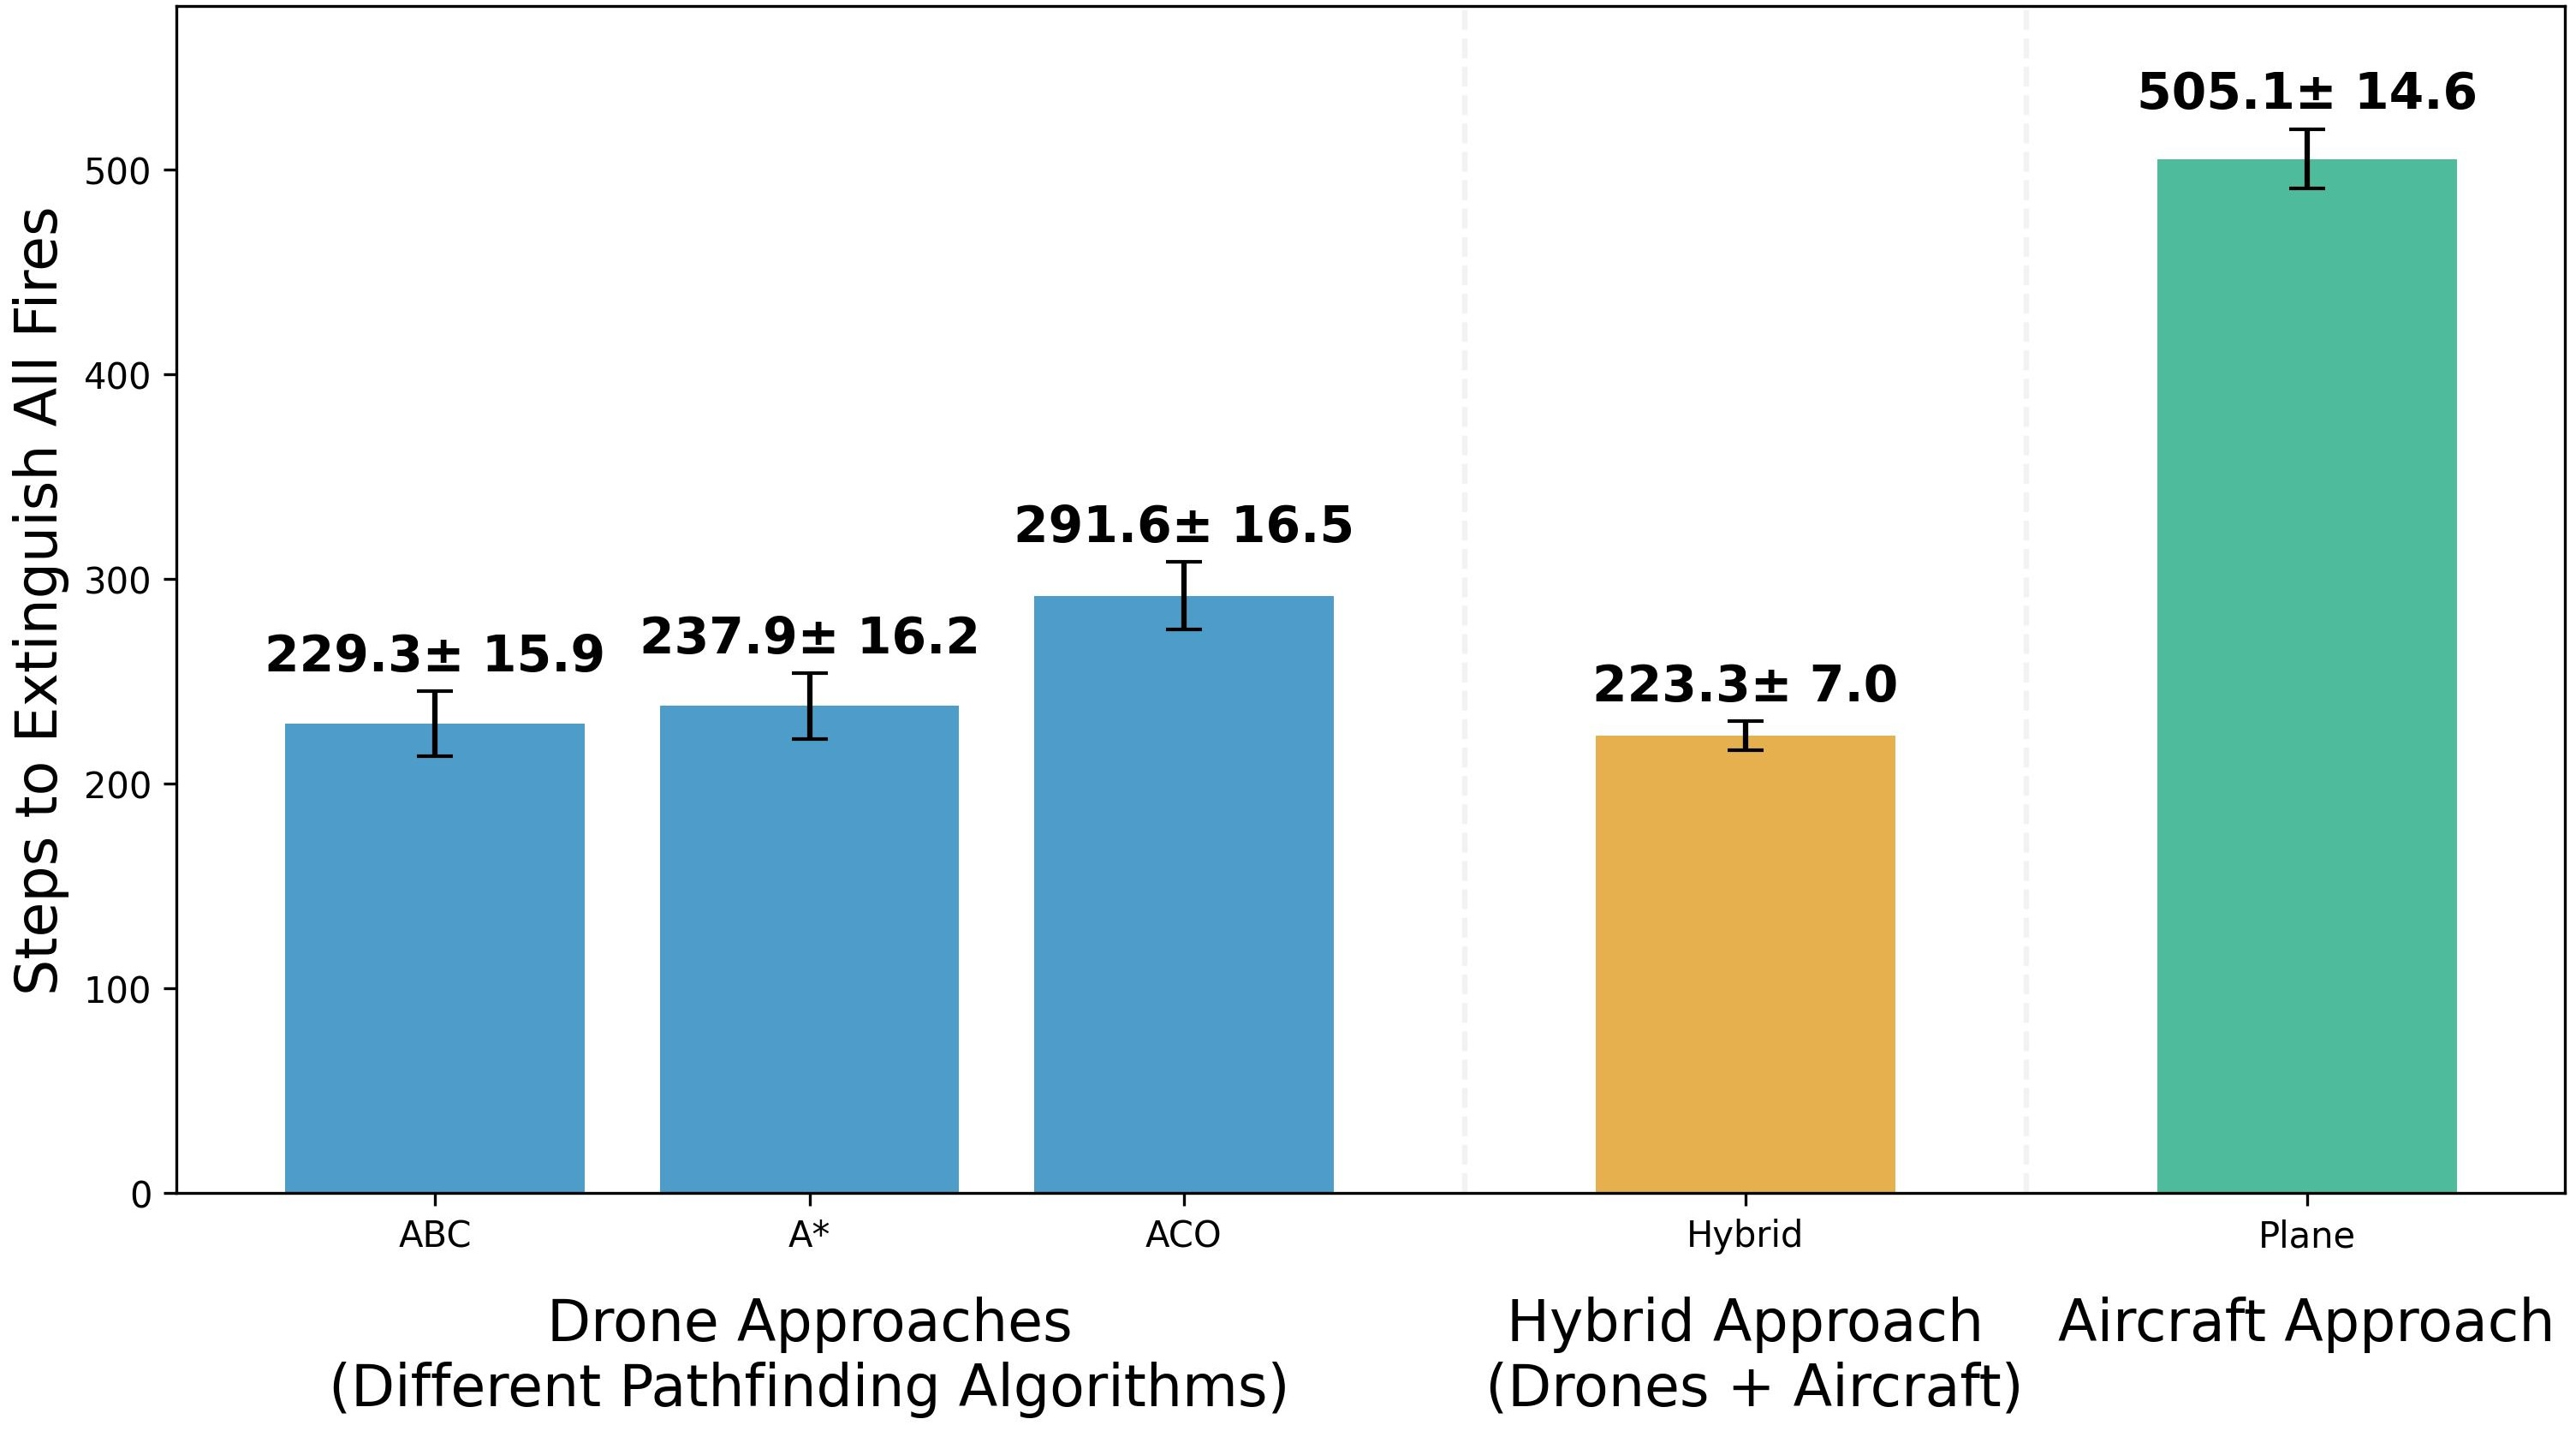
\includegraphics[width=1\linewidth]{figures/fire_extinction_comparison.jpeg}
    \caption{Mean Fire Extinction Time with 95\% Confidence Intervals}
    \label{fig:comparitive_analysis}
\end{figure}

\subsection{Resource Analysis}
\label{sec:resource}

Figure~\ref{fig:resources_analysisBIG} reports average water use, energy/fuel consumption, and emissions per simulation with a 95\% confidence interval and error bars. It is evident that the plane approach is by far the most expensive (€62,100) and pollutant approach in terms of water usage (877,500L) and CO\textsubscript{2} emissions (218,800 kg). Given the significantly different resource usages, the values are displayed in log scale to make them more comparable. Additionally, the cost factor is significantly higher than the compared approaches. The values for the plane approach go in line with the finding that the plane did not manage to condemn the fire in the given 1000-step time-frame. Figure~\ref{fig:comparitive_analysislineplot} demonstrated the downward trend of the slope indicated that the plane might manage to condemn the fire eventually, therefore making the simulation converge. However, although possibly being able to condemn the fire, the plane approach is inferior to the drone's resource management abilities. Drones generated the lowest emissions and resource usage, supporting their role in sustainable firefighting. Accordingly, the hybrid system, despite higher emissions, achieved the fastest containment and speed-sustainability trade-off (see Figure:~\ref{fig:computational_complexity_comparison}). When analyzing cost and water parameters, the same logic applies: drone approaches outperform their competitors, but the hybrid approach still significantly outperforms the plane approach. Table~\ref{tab:resource_usage} summarizes these findings for improved readability. 

\begin{figure}[htbp]
    \centering
    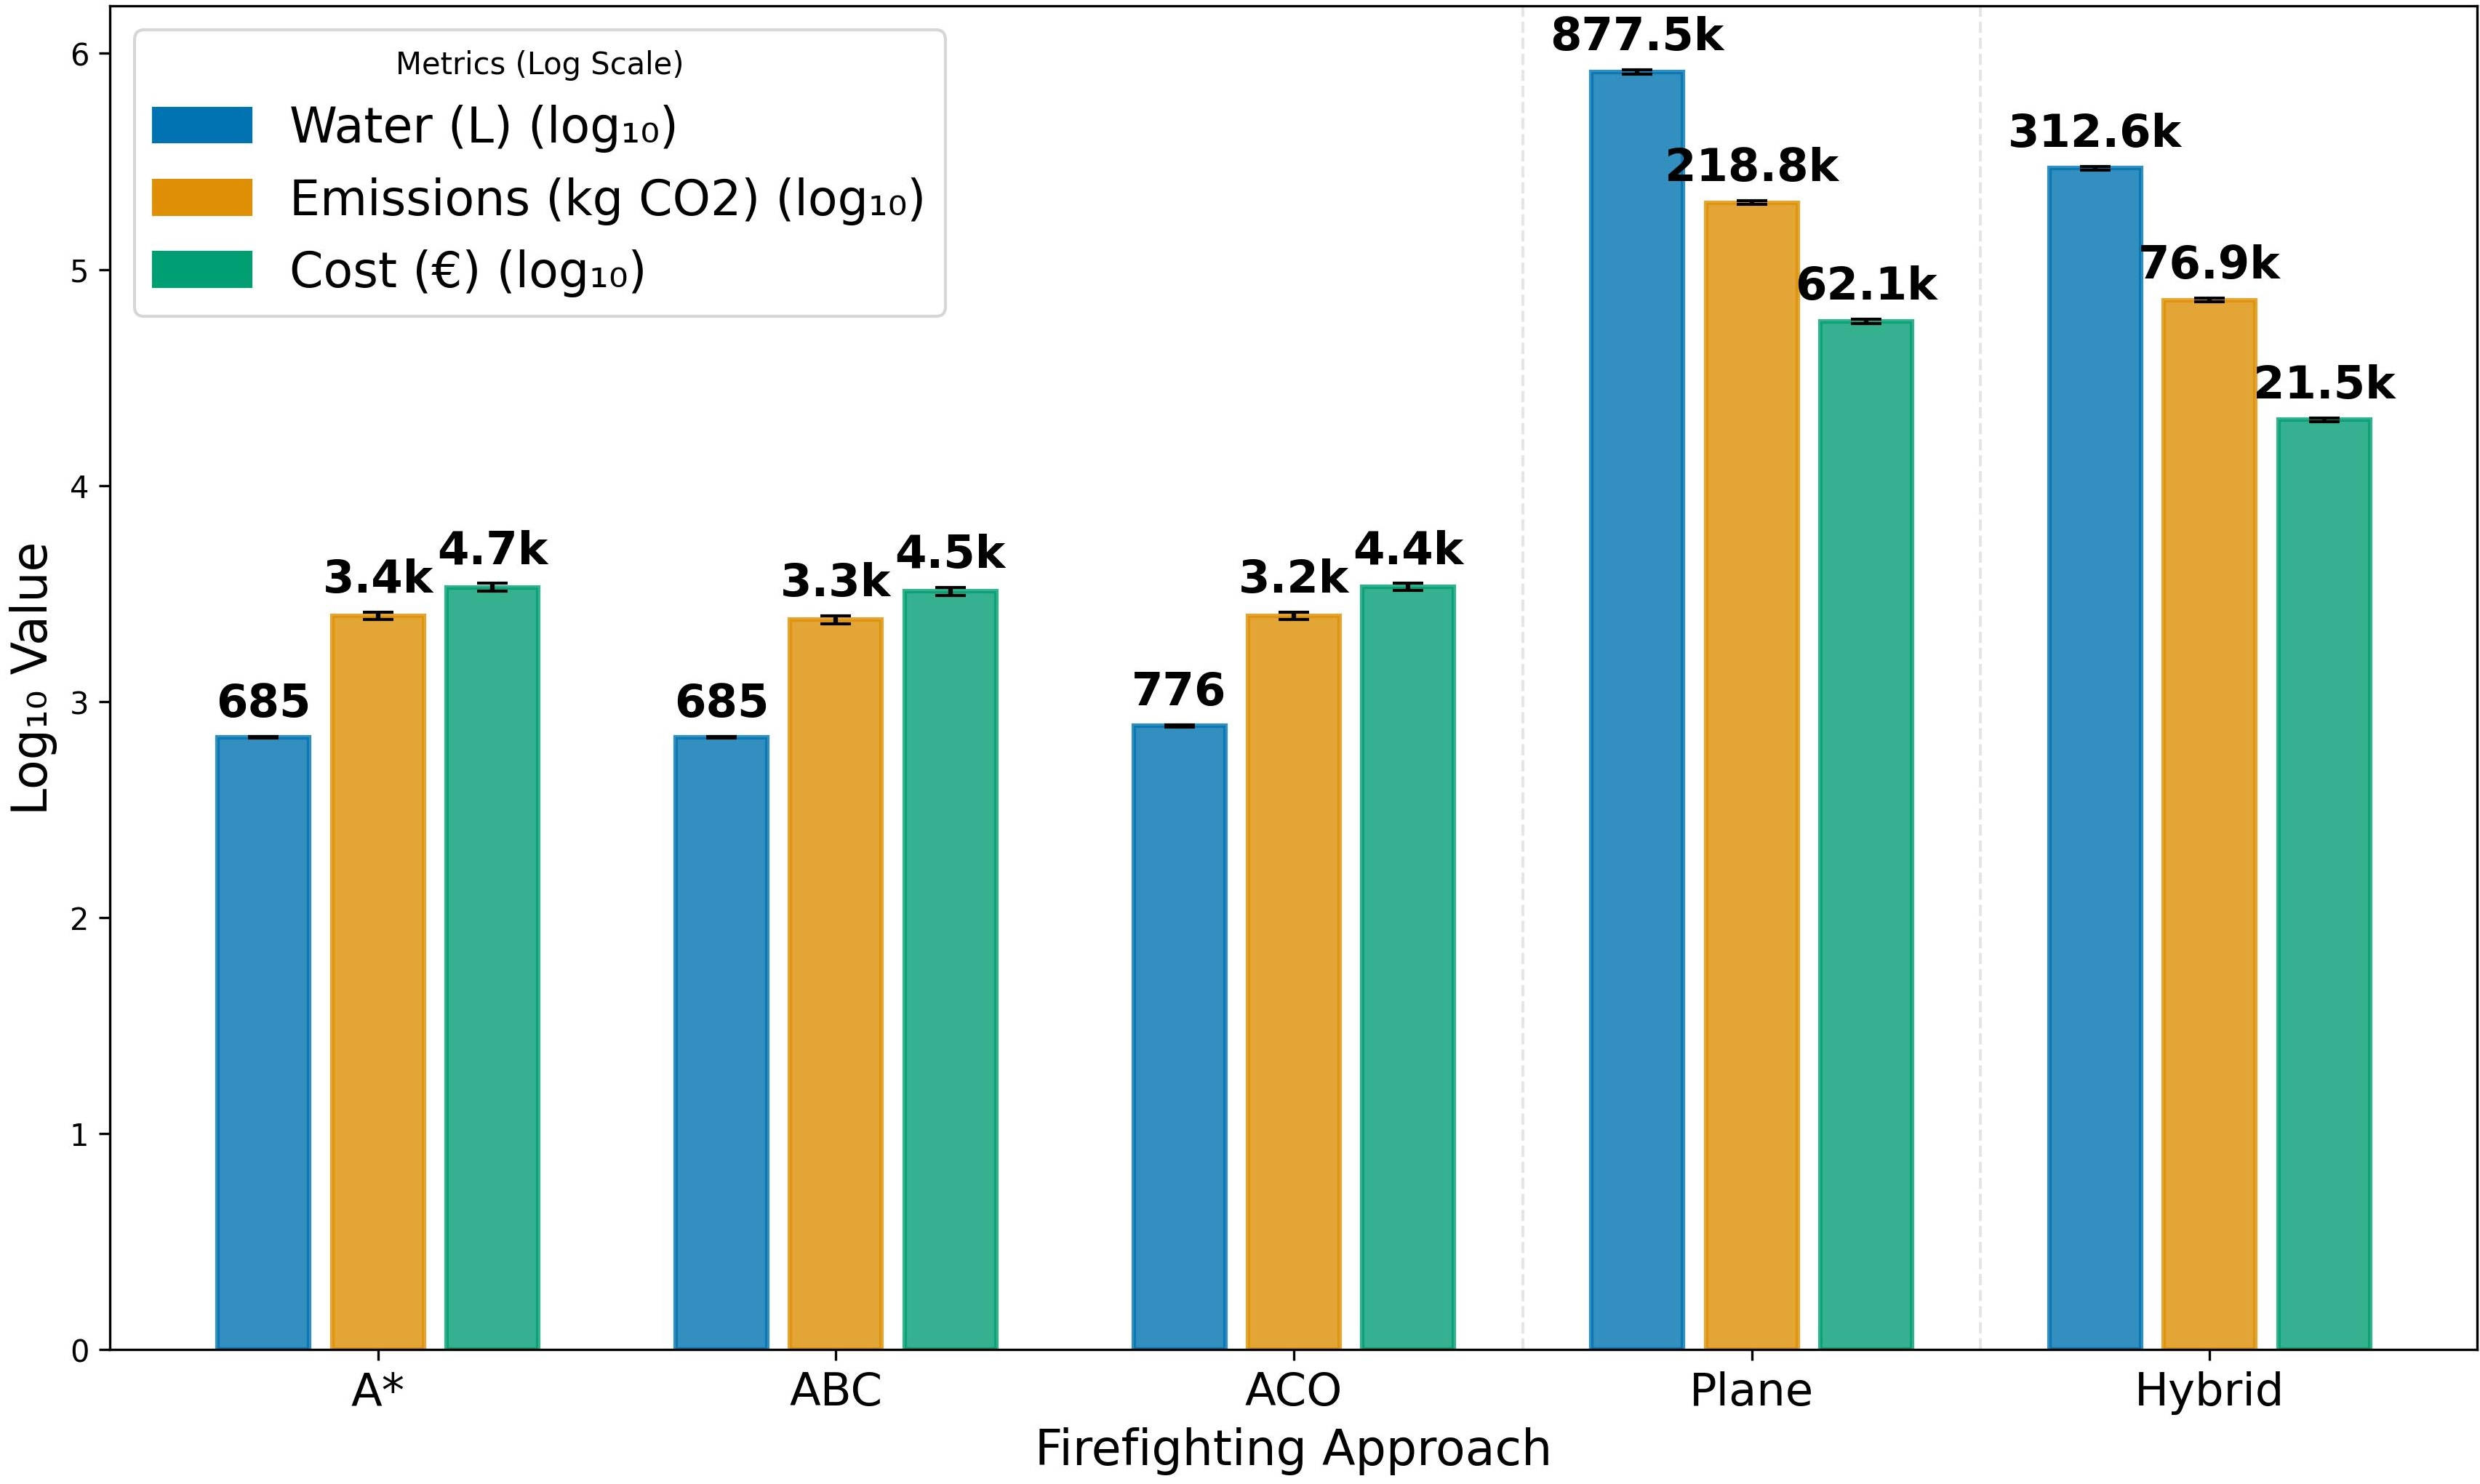
\includegraphics[width=1\linewidth]{figures/resource_analysis_log.jpeg}
    \caption{Comparative Analysis of Resource Usage and Environmental Impact by Approach (Log Scale)}
    \label{fig:resources_analysisBIG}
\end{figure}

\begin{table}[htbp]
\centering
\caption{Resource usage and environmental impact by firefighting approach. Drone methods use substantially less water, emit fewer CO\textsubscript{2} emissions, and cost significantly less than plane and hybrid approaches.}
\label{tab:resource_usage}
\begin{tabular}{lSSS}
\toprule
\textbf{Approach} & {\textbf{Water (L)}} & {\textbf{Emissions (kg CO\textsubscript{2})}} & {\textbf{Cost (€)}} \\
\midrule
\multicolumn{4}{l}{\textit{Drone Approaches}} \\
A* & 685 & 3400 & 4700 \\
ABC & 685 & 3300 & 4500 \\
ACO & 776 & 3200 & 4400 \\
\midrule
Plane & 877500 & 218800 & 62100 \\
Hybrid & 312600 & 76900 & 21500 \\
\bottomrule
\end{tabular}
\end{table}


\subsection{Computational Complexity}

\label{sec:computational_complexity}

Figure~\ref{fig:computational_complexity_comparison} presents the average simulation time required by each path-finding algorithm (1000 simulation steps). Computational efficiency is a key factor when deploying such systems; while some algorithms may find the fastest route, their high computational cost can be a significant trade-off. The results indicate that all tested path-finding methods achieved comparable performance levels, with average runtimes ranging from 0.48 seconds (Hybrid) and 1.71 seconds (A*), based on 1000 simulation iterations.


\begin{figure}[!htbp]
    \centering
    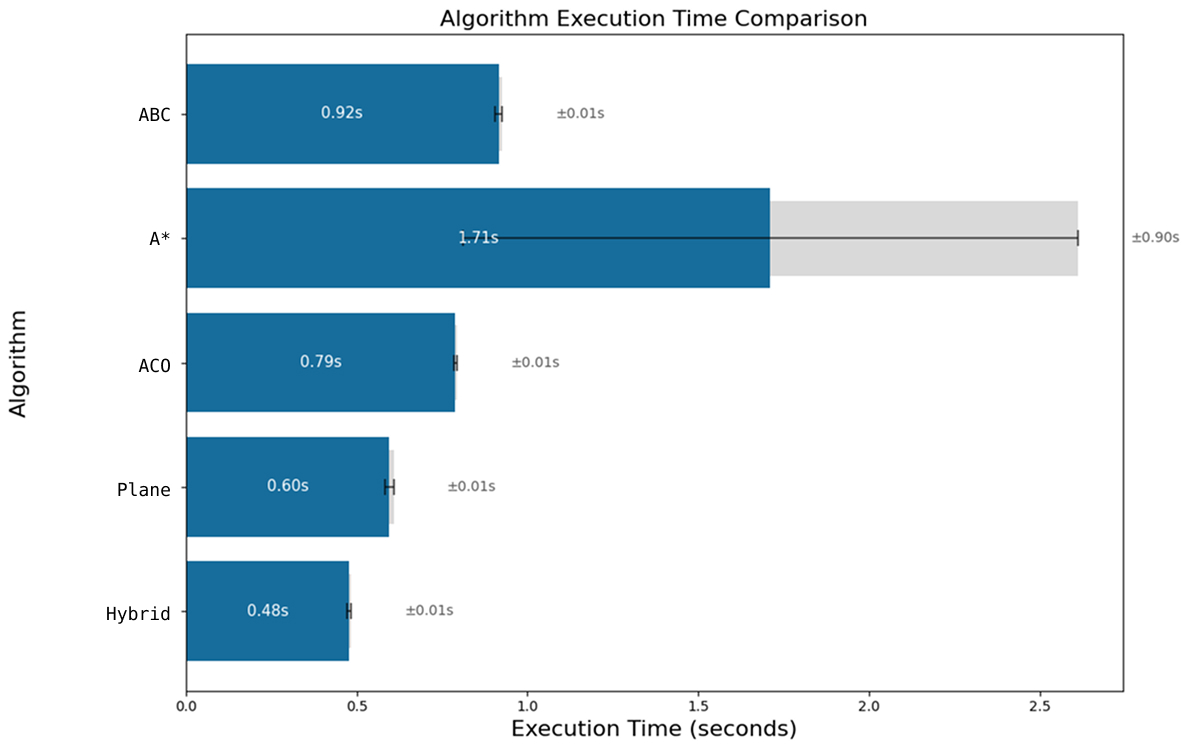
\includegraphics[width=1\linewidth]{figures/computational.jpg}
    \caption{Computational Complexity Comparison}
    \label{fig:computational_complexity_comparison}
\end{figure}

\subsection{Fire Risk Clustering and Analysis}
\label{sec:risk_assesment}

Figure~\ref{fig:risk_assesment} presents a fire risk analysis based on post-simulation data, where DBSCAN was primarily used to detect high-risk zones—areas where fires repeatedly re-ignited or were slow to extinguish. K-Means was applied only when DBSCAN failed to form meaningful clusters. The highlighted scenario shows a plane approach that did not converge within the 1000-step limit, emphasizing the need for adaptive fire response tactics. Figure~\ref{fig:risk_assesment} illustrates a clear correlation between fire density and assigned risk levels. Areas with a higher concentration of uncontained fires are classified with higher risk scores (86.6 and 61), compared to largely contained regions (38.7, 51.2, and 56.6). These results provide evidence that the risk assessment methodology effectively distinguishes between high-risk and low-risk areas, validating its potential for data-driven risk analysis and targeted intervention strategies. Ultimately, this supports the development of more complex and adaptive suppression behaviors.

\begin{figure}[!htbp]
    \centering
    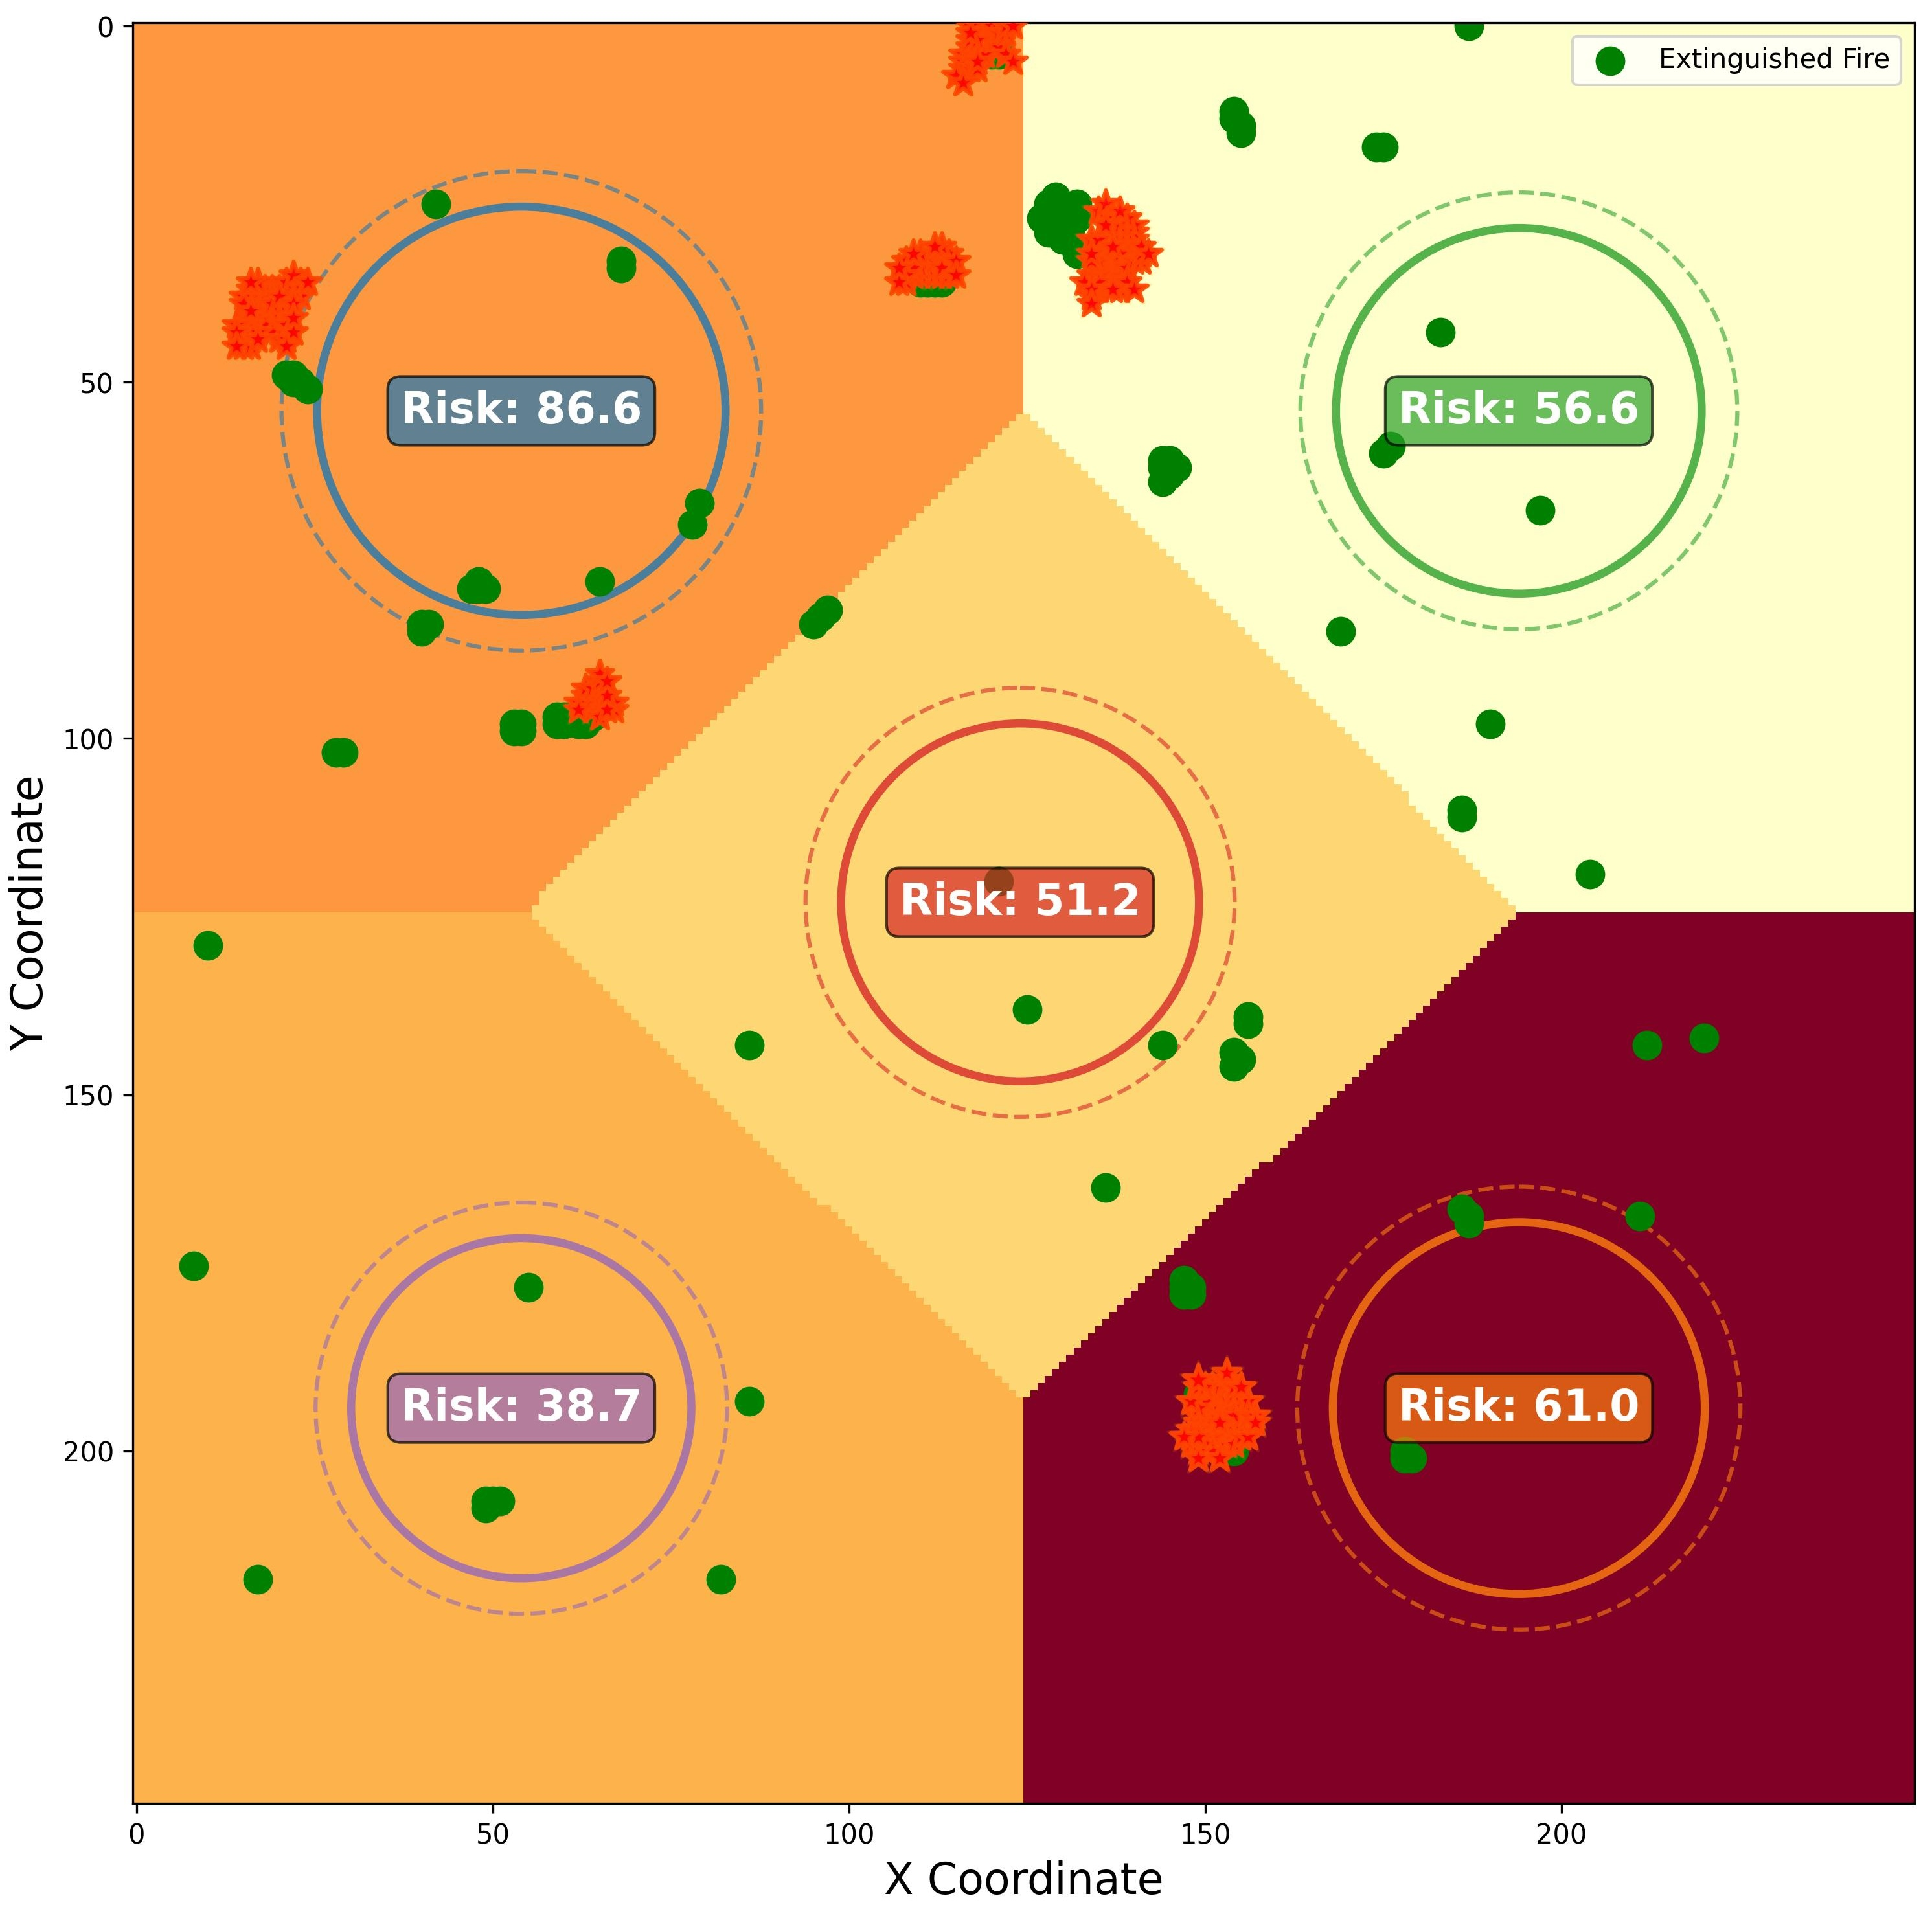
\includegraphics[width=1\linewidth]{figures/enhanced_fire_risk_analysis.jpeg}
    \caption{Fire risk assessment using DBSCAN clustering analysis on plane agent data. The environment is segmented into 5 distinct risk zones based on fire intensity, suppression delay, and spatial coordinates. Higher risk scores (86.6, 61) indicate areas with concentrated uncontained fires, while lower scores (38.7, 51.2, 56.6) represent regions with more successful suppression.}
    \label{fig:risk_assesment}
\end{figure}

%validation of why 50 fire agents - what happens if there are more fireagents
% faster suppression is better as firs grow further

The results hold under the assumption of initiating the simulation with 50 fires as the start; this value resulted as the best trade-off in simulation runtime and emergent patterns, as illustrated in Table~\ref{tab:fire_count_analysis}. The analysis over 10 independent simulations demonstrates that 50 fires provides sufficient complexity to observe meaningful fire dynamics and containment behaviors (99.0\% containment rate) while maintaining computational efficiency (0.71 seconds runtime). This configuration proves to be a representative value that captures emergent fire spread patterns without overwhelming the suppression system, while also being small enough to enable running the simulation 1000 times for robust statistical analysis, unlike higher fire counts (500-1000), which result in bad performing scenarios and significantly longer runtimes (20-65 seconds). 

\begin{table}[htbp]
    \centering
\caption{Fire Count Analysis Results (average results based on 10 independent simulations)}
    \label{tab:fire_count_analysis}
    \sisetup{
        separate-uncertainty = true,
        table-align-uncertainty = true
    }
    \begin{tabular}{
        S[table-format=4.0, round-precision=0, round-mode=places]  %* Forces integer display
        S[table-format=2.2(2), round-precision=2, round-mode=places]
        S[table-format=5.1(1), round-precision=1, round-mode=places]
        S[table-format=+5.1, round-precision=1, round-mode=places]
    }
        \toprule
        {Initial Fires} & {Runtime (s)} & {Fires After 1000 Steps} & {Containment (\%)} \\
        \midrule
        10   & 0.56    & 0.0          & 100.0   \\
        50   & 0.71    & 0.5          & 99.0    \\
        100  & 1.02    & 0.2          & 99.8    \\
        500  & 20.96   & 14380.4      & -2776.1 \\
        1000 & 65.08   & 30877.1      & -2987.7 \\
        \bottomrule
    \end{tabular}
\end{table}


\subsection{Summary of the Results}

Concluding, these results address the main research question by providing evidence on how agent-modeling can be used to evaluate and optimize aerial wildfire suppression strategies. This developed simulation model can be customized to specific parameters, making it a valid tool for evaluating suppression strategies. The exploratory machine learning approach provides further evaluation possibilities.
The simulation results on pathfinding behavior show areas of resource constraints, which can be used to adapt and optimize suppression strategies accordingly (RQ1).
While ABM can not provide proof, the established model provides evidence on emergent behavioral patterns defined by agent characteristics. 
Results demonstrate that drone approaches are cheaper, more consistent, and more sustainable (addressing RQ2) than plane approaches.
Figure~\ref{fig:comparitive_analysis} and Table~\ref{tab:resource_usage} suggest that the hybrid approach may demonstrate an optimal trade-off between sustainability and effectiveness (addressing RQ3). Particularly in extreme wildfire scenarios, even marginal improvements in suppression speed are critical. This integrated ABM framework establishes a foundation for transparent, data-driven fire suppression strategy evaluation applicable to real-world scenarios.

\section{Discussion}
\label{sec:discussion}
The main goal of this thesis was to evaluate the effectiveness of autonomous drone swarms in wildfire prevention, comparing them to traditional manned aircraft and hybrid approaches. The study aimed to assess these strategies based on suppression efficiency, emissions, operational cost, and water usage using a custom agent-based simulation framework. The project also pursued exploring the use of nature-inspired path-finding algorithms and unsupervised learning for enhancing decision-making in complex, dynamic fire environments.
\subsection{Interpretation of Key Findings}

The simulation results reveal significant performance differences across suppression approaches. Drone-only systems achieved fire containment in under 300 steps on average, while plane-only approaches consistently failed to converge within the simulation timeframe. Hybrid configurations demonstrated the fastest and most consistent performance, suggesting real-world applicability through plane-drone collaboration.

The cost analysis showed drone-only systems to be the most cost-efficient due to lower maintenance, fuel, and infrastructure requirements. Hybrid configurations, while fastest, still produced high costs due to the need for runways and refuel stations. These findings align with previous research employing new ways to fight wildfires and showing their potential \citep{fireBalls} but go further by simulating these metrics in a direct comparison.

Path-finding visualization results illustrated that the algorithms were functionally integrated and generated distinct emergent behavior, validating their integration in the simulation.
All three path-finding methods (A*, ACO, ABC) demonstrated comparable performance with acceptable computational complexity, indicating the simulation's robustness and adaptability. These findings support the trend toward electrified, decentralized suppression systems \citep{Saffre2022,stolaroffEnergyUseLife2018}, while demonstrating that hybrid approaches may offer the most practical balance between speed, consistency, and resource efficiency for real-world wildfire management.

\subsection{Limitations}

While the simulation produced clear trends, it operates under several assumptions and simplifications inherent in the simulation.

\paragraph{Parameter Constraints} The two-dimensional environment introduces dimensional constraints, which lack realistic properties. Especially for aerial vehicles, a three-dimensional environment is preferable, enabling the capture of altitude-dependent factors such as visibility, wind effects, and water/retardant dispersal patterns. 
Additionally, incorporating realistic obstacles, dynamic weather patterns, and potentially external data sources like satellite imagery would improve the model's accuracy and complexity. The absence of seasonality is another limitation worth addressing in future developments, as the true nature of wildfires is inherently seasonal.
Similarly, both the parameters for the drone and the plane agent were initialized as fixed values, whereas in reality these values are much more dynamic, with flight speed changing based on environmental factors and operational focus. Logically, the speed for \textit{firefighting} should be different from \textit{approaching the fire site}.
Additionally, fixed cost and emission parameters are used, whereas in reality these values fluctuate and depend on factors such as time of day and location. Location-specific parameters would yield drastically different results. For instance, electricity prices and emissions vary significantly across countries; Germany has noticeably higher electricity prices than Hungary as shown in Figure~1 \citep{ElectricityPriceStatistics}. While average values serve as a reasonable indicator for the scope of this research, incorporating more realistic and adaptive parameters is valuable for future development.
\paragraph{Machine Learning Integration} While the model lays the foundation for meaningful AI implementation in the future, the agents are still lacking intelligent behavior. The path-finding algorithms could be seen as intelligent behavior, since they use swarm properties to make decisions that appear smart. However, no autonomous decision-making framework is integrated. The risk assessment explored this direction: being a model-wide analyzer, which makes the drones all-knowing instead of enabling individual intelligent decision-making, limits its potential benefits. More intelligent behavior could also result in too high computation time. Therefore, a trade-off between these two opposites has to be established to find an optimal solution.

\subsection{Contributions}
This thesis contributes an open-source, modular simulation environment that unifies drone and plane behavior, nature-inspired algorithms, emissions and cost modeling, and ML-based risk mapping. While prior work has focused on UAV coordination \citep{Afghah2019} or suppression techniques \citep{fireBalls}, this project integrates direct comparison and scenario testing. It works as a baseline to build upon, making the integration of potentially sustainable planes or other UAVs possible. It also demonstrates that performance trade-offs are essential when evaluating different approaches, with certain infrastructure limitations potentially becoming advantages depending on other parameters. This interdisciplinary synthesize highlights the potential of collaborative research in sustainable wildfire monitoring.
From a practical perspective, the findings challenge the binary thinking often applied to wildfire management solutions. Rather than treating drones and traditional aircraft as competing technologies, dynamic and collaborative approaches between a range of technologies should be considered.
The simulation framework provides a foundation for developing decision support tools.

\subsection{Future Research}

The motivation for this research is a tool in which environmental data is used as input, with seasonality, weather, and other unforeseen environmental changes taken into account. After simulating, the output would be an estimate of the cost and emissions that would be needed to effectively monitor the given environment. The tool can aid in deciding which firefighting approach to choose; based on differences in environments and local phenomena, the results change and provide valuable insight. 

This research provides a step in the right direction, motivating cheaper and more sustainable wildfire prevention techniques. Future development directions could include integrating realistic terrain, weather, and wind models; connecting to live data sources such as satellite data and weather APIs; applying more complex AI-driven decision-making such as deep reinforcement learning to enable unsupervised swarm behavior; incorporating human-swarm interaction drawing inspiration from current research while ensuring ethical implications and interactive planning \citep{lewisHumanFactorsIssues2012}; and implementing more realistic parameters such as adaptive cost, emission, and speed.

Logically, there are various possibilities in different directions. While it is beneficial to simulate the environment in greater complexity, there is a trade-off between overcomplicating the model by representing everything as realistically as possible and producing a fast, usable simulation. This fact must be carefully considered.

\section{Conclusion}

This thesis presents an integrated simulation framework for evaluating autonomous wildfire suppression strategies, combining agent-based modeling, nature-inspired path-finding, operational cost modeling, and machine learning-based risk analysis. By implementing drones, planes, and hybrid strategies all into a single simulation environment, the work enables a transparent comparison grounded in performance, sustainability, and cost-efficiency.

The main research question is comprehensively addressed through the ABM framework's ability to capture emergent behaviors, path-finding dynamics (RQ1), resource parameters, and effectiveness comparisons (RQ2) across suppression approaches, allowing quantification of effectiveness-sustainability trade-offs (RQ3).

The simulation results demonstrate that drone-based approaches significantly outperform traditional aircraft in both suppression speed and operational consistency, with the hybrid approach excelling at speed.

These findings challenge conventional binary thinking in wildfire management by demonstrating that collaborative approaches (drone + plane) offer superior performance characteristics.

This work contributes a modular open-source framework, enabling effective wildfire research without dismissing sustainability, encouraging a shift towards scalable, lower-emission fire response systems that reduce dependency on costly solutions through informed decision-making.

As wildfires continue to grow in frequency and intensity, there is an urgent need for adaptable, sustainable, and fast deployable solutions. The work presented here offers a foundation for future research and policymaking.

\bibliographystyle{apalike}
\bibliography{references}

\section*{Appendix}
\label{Appendix}
%TC:ignore
%ModelLogic
\label{app:modellogic}
\begin{figure}[H]
    \centering
    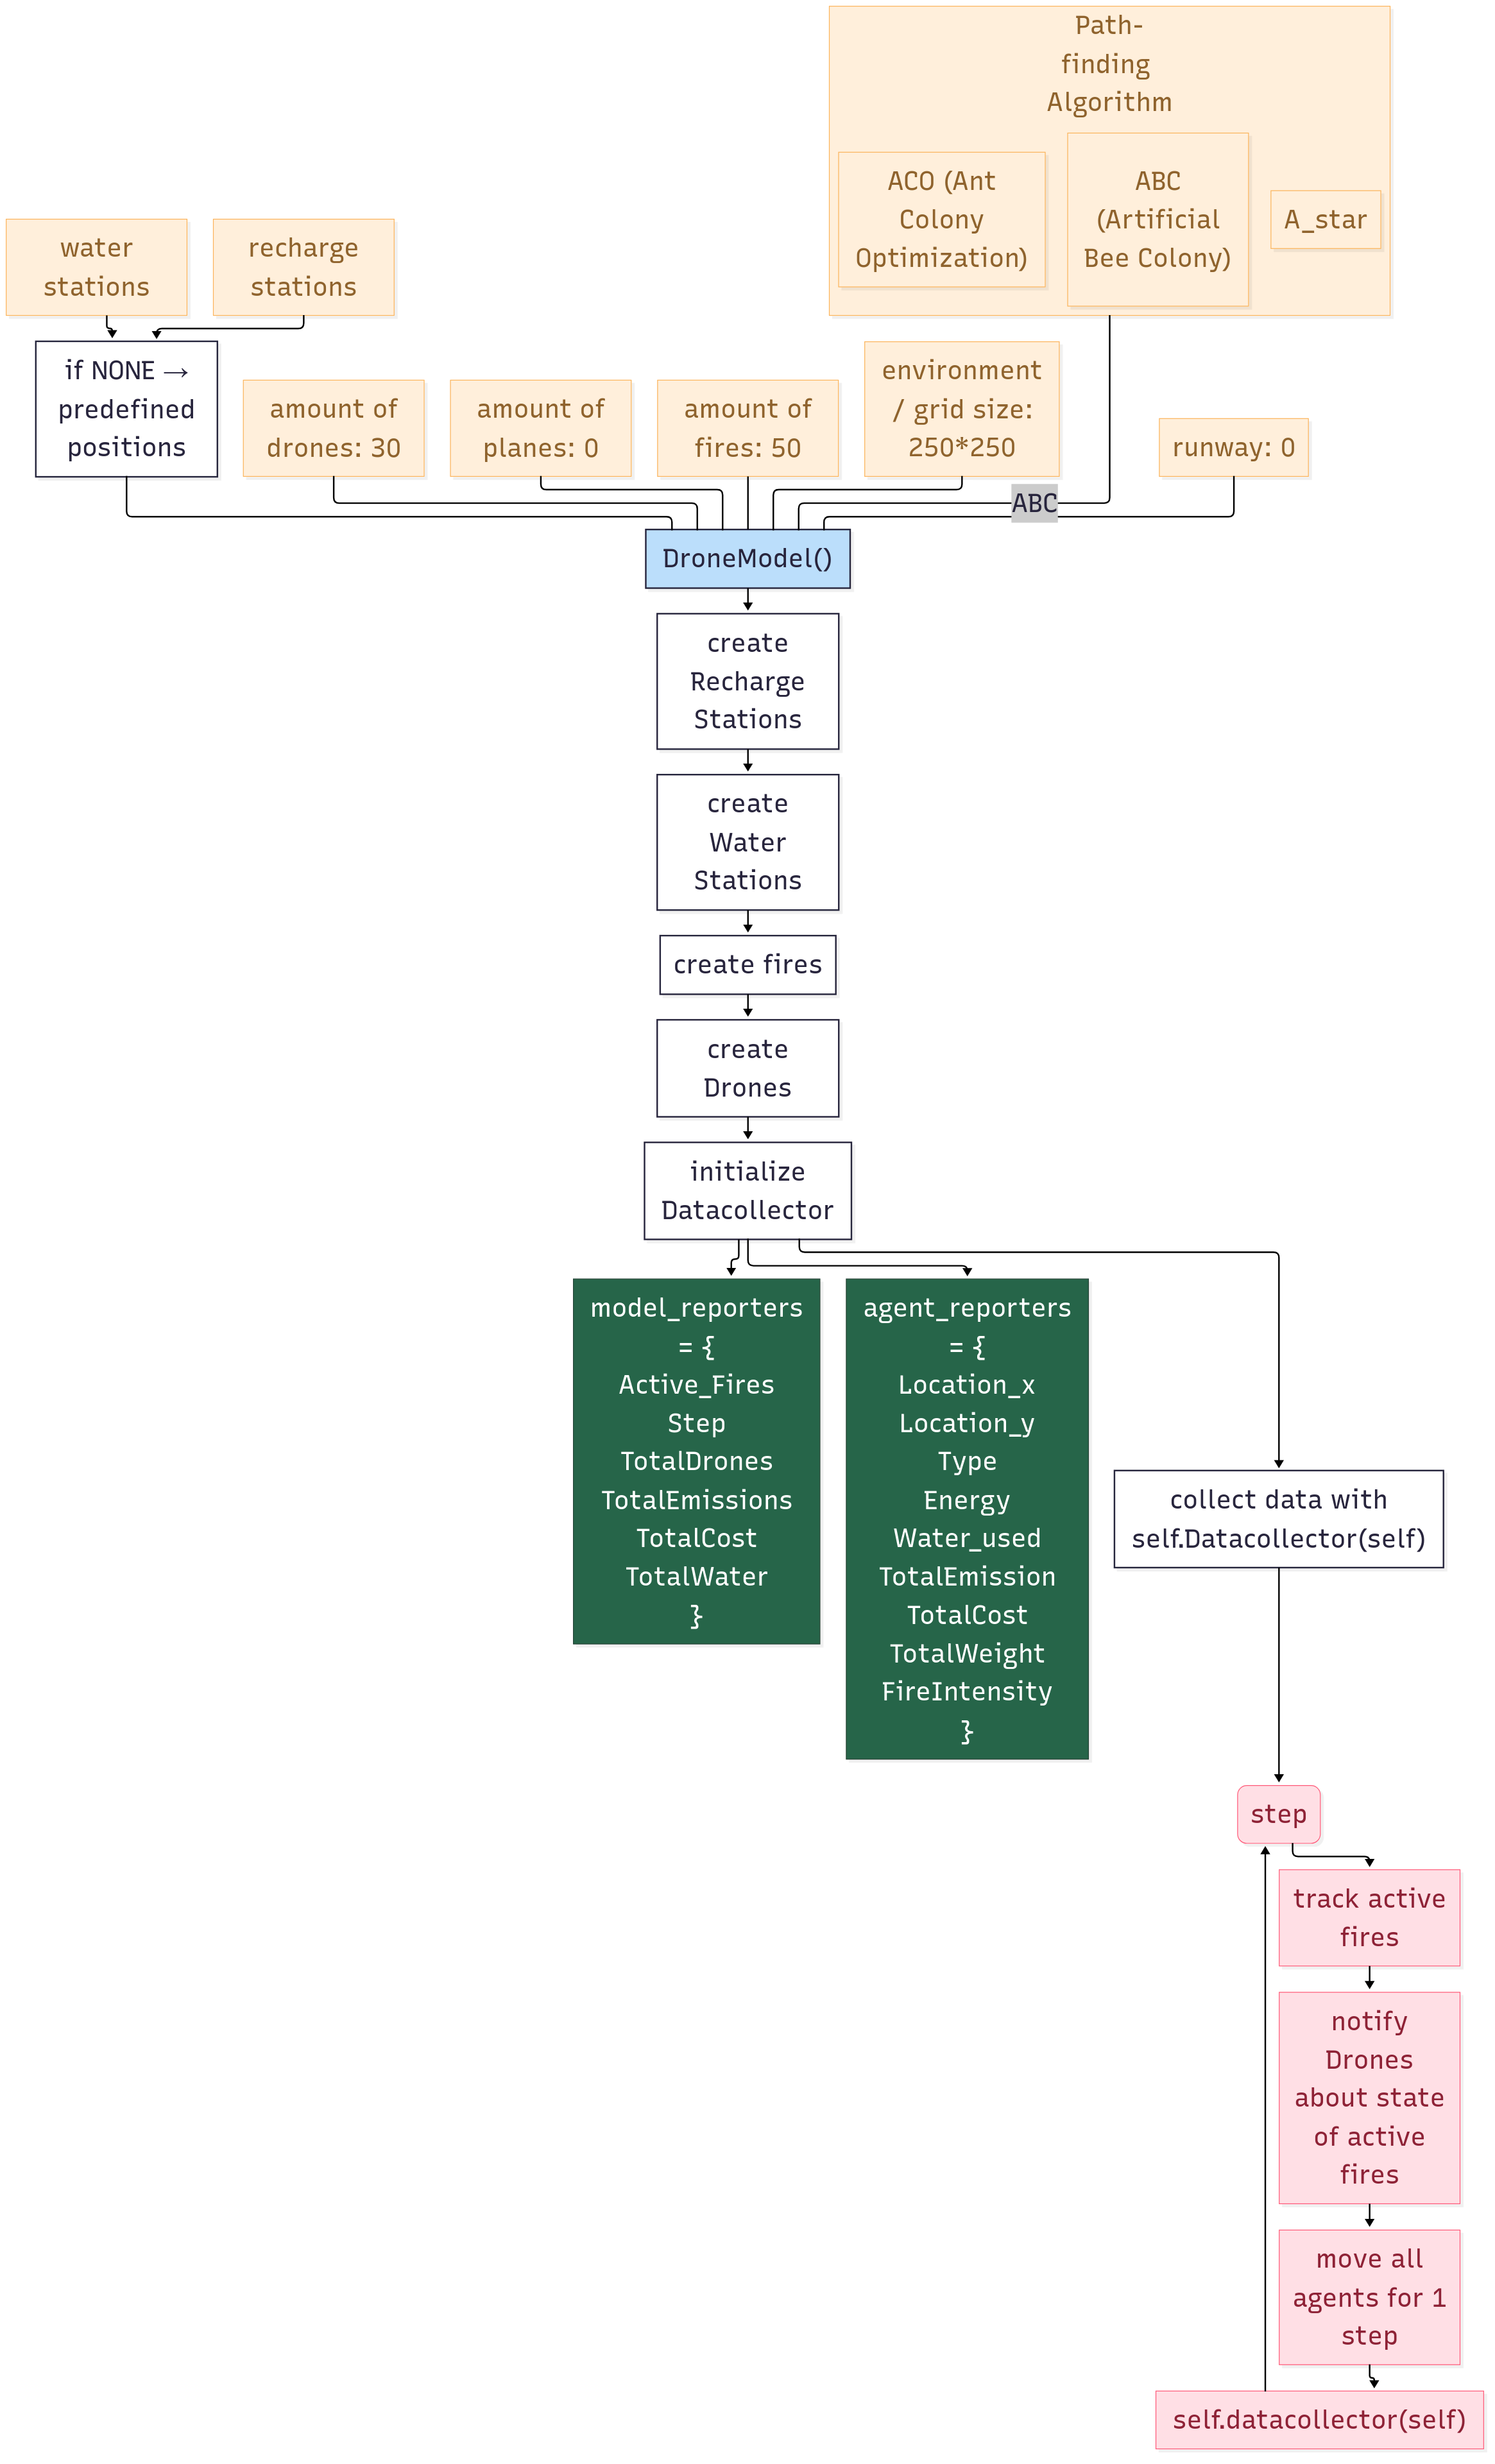
\includegraphics[width=1\textwidth]{figures/modellogic.png}
    \caption{Complete Model Architecture and Agent Interaction Logic}
    \label{fig:modellogic}
\end{figure}

\begin{table}[htbp]
\centering
\caption{Water Station Agent Parameters}
\label{tab:water_station_parameters}
\small
\begin{tabular}{@{}p{4cm}p{2cm}p{6cm}@{}}
\toprule
\textbf{Parameter Name} & \textbf{Default Value} & \textbf{Description} \\
\midrule
\multicolumn{3}{l}{\textbf{Initialization Parameters}} \\
\midrule
location & [x,y] & Position of the water station \\
capacity & \SI{1000}{\liter} & Maximum water capacity in liters \\
unique\_id & int & Unique identifier for the agent \\
typ & ``water\_station'' &  \\
active & T/F & Boolean indicating operational status \\
\midrule
\multicolumn{3}{l}{\textbf{Operational Parameters}} \\
\midrule
refill\_rate & \SI{20}{\liter} & Water refilled automatically per step \\
\midrule
\multicolumn{3}{l}{\textbf{Environmental Impact}} \\
\midrule
emissions\_factor & 0.20 & Emissions in kg of CO\textsubscript{2} per liter dispensed \\
total\_emissions & 0.0 & Total emissions accumulated \\
\midrule
\multicolumn{3}{l}{\textbf{Cost Metrics}} \\
\midrule
water\_cost & €0.00061 & Cost per liter \citep{waterPricing} \\
maintenance\_cost & €0.03 & Fixed operating cost per step \\
total\_cost & €0.0 & Cumulative cost of operations \\
\midrule
\multicolumn{3}{l}{\textbf{Usage Metrics}} \\
\midrule
total\_water\_provided & \SI{0}{\liter} & Total liters of water provided \\
refill\_events & 0 & Accumulated number of refill events \\
\bottomrule
\end{tabular}
\end{table}

\begin{table}[htbp]
\centering
\caption{Recharge Station Agent Parameters}
\label{tab:recharge_station_parameters}
\small
\begin{tabular}{@{}p{4cm}p{2cm}p{6cm}@{}}
\toprule
\textbf{Parameter Name} & \textbf{Default Value} & \textbf{Description} \\
\midrule
\multicolumn{3}{l}{\textbf{Initialization Parameters}} \\
\midrule
location & [x,y] & Position of the recharge station \\
unique\_id & int & Unique identifier for the agent \\
typ & ``recharge\_station'' & Agent type identifier \\
active & T/F & Boolean indicating active status \\
\midrule
\multicolumn{3}{l}{\textbf{Operational Parameters}} \\
\midrule
charge\_rate & 100 & Energy units provided per recharge step \\
\midrule
\multicolumn{3}{l}{\textbf{Environmental Impact}} \\
\midrule
emissions\_factor & 0.200 & Emissions in kg of CO\textsubscript{2} per kWh provided. The energy emission varies based on various factors. The given value is based on research done by \citet*{stolaroffEnergyUseLife2018} which shows energy emission efficiency in drones. \\
total\_emissions & 0.0 & Total emissions accumulated \\
\midrule
\multicolumn{3}{l}{\textbf{Cost Metrics}} \\
\midrule
electricity\_cost & €0.2872 & Electricity cost per kWh taken from the EU average in 2023 \citep{ElectricityPriceStatistics}. \\
maintenance\_cost & €0.05 & Fixed operational cost per step \\
total\_cost & €0.0 & Total operational cost accumulated \\
\midrule
\multicolumn{3}{l}{\textbf{Usage Metrics}} \\
\midrule
total\_energy\_provided & 0.0 & Total kWh of energy provided \\
recharge\_events & 0 & Accumulated number of recharge events \\
\bottomrule
\end{tabular}
\end{table}

\begin{table}[htbp]
\centering
\caption{Detailed parameter description of the fire agent}
\label{tab:fire_agent_parameters}
\small
\begin{tabular}{@{}p{4cm}p{2cm}p{6cm}@{}}
\toprule
\textbf{Parameter Name} & \textbf{Default Value} & \textbf{Description} \\
\midrule
\multicolumn{3}{l}{\textbf{Initialization Parameters}} \\
\midrule
location & [x,y] & Coordinates of the fire area \\
intensity & 5 & Fire intensity on a scale from 1 to 10 \\
size & 1 & Size of the fire (radius) \\
unique\_id & int & Unique identifier for the agent \\
typ & "fire" & Type identifier for the agent \\
active & T/F & Boolean indicating whether the fire is currently burning \\
age & 0 & Age of the fire in simulation steps \\
water\_applied & 0 & Total water applied to this fire \\
\midrule
\multicolumn{3}{l}{\textbf{Spreading Behavior}} \\
\midrule
spread\_probability & 0.05 & Base chance of spreading per step \\
last\_spread\_attempt & 0 & Step count of last spread attempt \\
spread\_cooldown & 10 & Minimum steps between spread attempts \\
\midrule
\multicolumn{3}{l}{\textbf{Methods and Behaviors}} \\
\midrule
apply\_water(water\_amount) & — & Reduces intensity, extinguishes fire if intensity $\leq 0.5$ \\
step() & — & Ages fire, increases intensity slightly, attempts spread \\
attempt\_spread() & — & Checks for nearby cells and spreads if possible \\
extinguish() & — & Manually sets fire as extinguished \\
\bottomrule
\end{tabular}
\end{table}

\begin{table}[htbp]
\centering
\caption{Runway Agent Parameters}
\label{tab:runway_parameters}
\small
\begin{tabular}{@{}p{4cm}p{2cm}p{6cm}@{}}
\toprule
\textbf{Parameter Name} & \textbf{Default Value} & \textbf{Description} \\
\midrule
\multicolumn{3}{l}{\textbf{Initialization Parameters}} \\
\midrule
location & [x,y] & Grid location of the runway \\
typ & ``runway'' & Type identifier for the agent \\
is\_occupied & T/F & Boolean indicating occupancy status \\
occupying\_plane & None & Reference to the plane currently on the runway \\
\midrule
\multicolumn{3}{l}{\textbf{Resource Capacities}} \\
\midrule
fuel\_capacity & \SI{10000}{\liter} & Maximum amount of fuel the runway can store \\
fuel\_level & \SI{10000}{\liter} & Current fuel level in the runway \\
water\_capacity & \SI{20000}{\liter} & Maximum amount of water the runway can store \\
water\_level & \SI{20000}{\liter} & Current water level in the runway \\
\midrule
\multicolumn{3}{l}{\textbf{Refill Rates (Per Step)}} \\
\midrule
fuel\_refill\_rate & \SI{200}{\liter} & Fuel replenished per simulation step \\
water\_refill\_rate & \SI{500}{\liter} & Water replenished per simulation step \\
\midrule
\multicolumn{3}{l}{\textbf{Environmental Impact Parameters}} \\
\midrule
fuel\_emissions\_factor & 0.2 kg & CO\textsubscript{2} emissions per unit of fuel provided \\
water\_emissions\_factor & 0.1 kg & CO\textsubscript{2} emissions per unit of water provided \\
total\_emissions & 0.0 kg & Cumulative emissions generated \\
\midrule
\multicolumn{3}{l}{\textbf{Cost Parameters}} \\
\midrule
fuel\_cost & €0.3 & Cost per unit of fuel provided \\
water\_cost & €0.05 & Cost per unit of water provided \\
maintenance\_cost & €0.5 & Operational maintenance cost per step \\
total\_cost & €0.0 & Accumulated operational costs \\
\midrule
\multicolumn{3}{l}{\textbf{Usage Statistics}} \\
\midrule
planes\_serviced & 0 & Total number of planes serviced \\
fuel\_provided & 0.0 & Total fuel supplied to planes \\
water\_provided & 0.0 & Total water supplied to planes \\
\bottomrule
\end{tabular}
\end{table}


%TC:endignore



\end{document}